%% ============================================================================
%% preamble.tex -- shared preamble, Quant Corpus Consolidation Committee
%% Ratified by FORMALIS (Round 0). Governed by /home/renaud/Models/NOTATION_CONTRACT.md
%% Usage: this file is \input at the very top of each volume, before
%% \begin{document}. It supplies the document class, packages, theorem
%% environments, and the mandated notation macros. Leads MUST use these
%% macros; raw retypings of contract symbols are contract violations.
%% ============================================================================

\documentclass[11pt]{book}

%% ---------------------------------------------------------------- packages
\usepackage[T1]{fontenc}
\usepackage[utf8]{inputenc}
\usepackage{amsmath}
\usepackage{amssymb}          % \varkappa, blackboard bold
\usepackage{amsthm}
\usepackage{mathtools}        % \DeclarePairedDelimiter, \coloneqq
\usepackage[margin=1in]{geometry}
\usepackage{graphicx}
\usepackage{xcolor}
\usepackage{tikz}
\usepackage{pgfplots}
\pgfplotsset{compat=newest}
\usepackage{booktabs}
\usepackage{enumitem}

%% ------------------------------------------------- theorem-like environments
%% Numbered within chapter; lemma/proposition/etc. share the theorem counter.
\theoremstyle{plain}
\newtheorem{theorem}{Theorem}[chapter]
\newtheorem{lemma}[theorem]{Lemma}
\newtheorem{proposition}[theorem]{Proposition}
\newtheorem{corollary}[theorem]{Corollary}
\theoremstyle{definition}
\newtheorem{definition}[theorem]{Definition}
\newtheorem{example}[theorem]{Example}
\newtheorem{assumption}[theorem]{Assumption}
\theoremstyle{remark}
\newtheorem{remark}[theorem]{Remark}

%% -------------------------------------------------------- bra-ket (mandated)
%% Hand-rolled; replicates the braket-package syntax used by the canonical
%% spine (ImpliedLocalVol): \braket{\phi(m)|\beta} takes ONE argument with a
%% literal | inside. Deliberately NOT the physics package (whose \braket takes
%% two arguments and which redefines \div, \Re, ...).
\newcommand{\ket}[1]{\mathinner{\lvert #1 \rangle}}
\newcommand{\bra}[1]{\mathinner{\langle #1 \rvert}}
\newcommand{\braket}[1]{\mathinner{\langle #1 \rangle}}
\newcommand{\ketbra}[2]{\ket{#1}\!\bra{#2}}
\newcommand{\featket}{\ket{\phi(\mln)}}          % feature ket |phi(m)>
\newcommand{\parket}{\ket{\beta}}                % parameter ket |beta>

%% ------------------------------------- mandated volatility decomposition
%% m = ln(K/F);  sigma_smile(m,T);  sigma_ATM(l_F,T),  l_F = ln(F/F_ref).
\newcommand{\mln}{m}                             % strike log-moneyness ln(K/F)
\newcommand{\lF}{\ell_F}                         % forward log-level ln(F/F_ref)
\newcommand{\Fref}{F_{\mathrm{ref}}}             % reference forward (anchor)
\newcommand{\ssm}{\sigma_{\mathrm{smile}}}       % smile component, args (m,T)
\newcommand{\satm}{\sigma_{\mathrm{ATM}}}        % ATM component, args (l_F,T)
\newcommand{\satmi}[1]{\sigma_{\mathrm{ATM},#1}} % per-name ATM vol (basket, C1)
\newcommand{\lFi}[1]{\ell_{F,#1}}                % per-name forward log-level ln(F_i/F_{ref,i}) (C1 note)
\newcommand{\Frefi}[1]{F_{\mathrm{ref},#1}}      % per-name reference forward (C1 note)
\newcommand{\volslope}{\mathrm{vol.slope}}       % := d(satm)/d(lF)  (C2)
\newcommand{\sloc}{\sigma_{\mathrm{loc}}}        % Dupire local vol
\newcommand{\sref}{\sigma_{\mathrm{ref}}}        % kernel reference vol

%% ------------------------------------------------------------ normal glyphs
\newcommand{\npdf}{\varphi}                      % standard normal pdf (R5)
\newcommand{\ncdf}{N}                            % standard normal CDF (R5)
\newcommand{\Nrm}{\mathcal{N}}                   % Gaussian LAW N(mu,Sigma); \ncdf reserved for the scalar CDF (R5)

%% --------------------------------------- Vol I Ch 4 (Calibration) local block
\newcommand{\parvec}{\vartheta}                  % calibration parameter vector (I.4); NOT BS theta (Greeks table)
%% \lFi is defined once in the volatility-decomposition block above (C1 note); shared by I.4 and II.1.
\newcommand{\gDurr}{\mathfrak{g}}                % Durrleman butterfly function (I.4); NOT the metadata slot g
\newcommand{\Ninstr}{N_{\mathrm{ins}}}           % instrument count (I.4); NOT the normal CDF N(x)

%% ------------------------------------------------------------------- Greeks
\newcommand{\vega}{\nu}                          % BS vega dC/dsigma (R2)
\newcommand{\Vanna}{\mathrm{Vanna}}
\newcommand{\Volga}{\mathrm{Volga}}
\newcommand{\Gadj}{\Gamma_{\mathrm{adj}}}        % total (smile-adjusted) gamma

%% ------------------------------------------------- multi-name (Vol II) block
\newcommand{\sB}{\sigma_B}                       % basket vol
\newcommand{\sbmean}{\bar\sigma}                 % (sigma1+sigma2)/2
\newcommand{\Cega}{\mathrm{Cega}}                % correlation sensitivity
\newcommand{\VB}{\mathcal{V}_B}                  % basket vega per vol point
\newcommand{\shvega}{\mathrm{ShadowVega}}
\newcommand{\shdelta}{\mathrm{ShadowDelta}}
\newcommand{\stickyrho}{\textnormal{sticky-}\ensuremath{\rho}} % d(rho)=0 convention (R4); works in text and math
\newcommand{\stickycvc}{\textnormal{sticky-CVC}}               % d(xi)=0 convention (R4); works in text and math
\newcommand{\SigmaM}{\Sigma_M}                   % Margrabe volatility
\newcommand{\omM}{\omega_M}                      % Sigma_M*sqrt(T), replaces nu (R2)
\newcommand{\symk}{\varkappa}                    % Margrabe symmetry constant, replaces k (R3.3)
\newcommand{\SchurC}[2]{\mathrm{Schur}_{#1}\!\left(#2\right)} % Schur complement

%% -------------------------------------------------------- calculus & algebra
\newcommand{\dd}{\mathrm{d}}                                  % upright differential
\newcommand{\pd}[2]{\frac{\partial #1}{\partial #2}}          % partial derivative
\newcommand{\pdd}[2]{\frac{\partial^2 #1}{\partial #2^2}}     % second partial
\newcommand{\pdc}[3]{\frac{\partial^2 #1}{\partial #2\,\partial #3}} % cross partial
\newcommand{\td}[2]{\frac{\dd #1}{\dd #2}}                    % total derivative
\newcommand{\atfixed}[2]{\left.#1\right|_{#2}}                % held-fixed bar, e.g. \atfixed{\pd{\SigmaM}{\sigma_1}}{\xi}
\newcommand{\E}{\mathbb{E}}
\newcommand{\Var}{\operatorname{Var}}
\newcommand{\Cov}{\operatorname{Cov}}
\DeclarePairedDelimiter{\abs}{\lvert}{\rvert}
\DeclarePairedDelimiter{\norm}{\lVert}{\rVert}

%% ============================================================================

%% ============================================================================
%% Title, front matter, and document start (assembled by MATTHIAS)
%% ============================================================================
\title{Quantitative Volatility Corpus\\[0.5em]\Large Volume~II: Multi-Name Volatility, Correlation, and Numerical Methods}
\author{Quant Corpus Consolidation Committee}
\date{}

\begin{document}

\frontmatter
\maketitle
\tableofcontents

\mainmatter
%% ============================================================================
%% Vol II, Chapter 1 -- Basket volatility and the correlation-volatility relation
%% Conforms to NOTATION_CONTRACT.md (FORMALIS, Round 0). Macros from build/preamble.tex.
%% ============================================================================

\chapter{Basket Volatility and the Correlation--Volatility Relation}
\label{ch:vol2-basket}

A long basket (or index) straddle is \emph{long correlation}: the basket
volatility rises when the constituents move together, so the position is worth
more when they correlate. The opposite side of that risk is the dispersion
trade --- long single-name volatility, short basket volatility --- which is
short correlation. This chapter builds the objects with which that risk is
measured and re-marked: the basket volatility identity, the basket vol spread
$\xi$, the CVC spread (the price of the dispersion package), the exact relation
$\rho = \rho(\sigma_1,\sigma_2,\xi)$, and the correlation sensitivity $\Cega$.
It also extends the no-arbitrage ladder to two names --- the rungs
$\xi \ge 0$ (equivalently $\rho \le 1$) and $\rho \ge -1$ --- and fixes the
two re-marking conventions, \stickyrho{} and \stickycvc, whose difference
generates the shadow Greeks of the routed-sensitivities chapter. A single
worked example ($\sigma = 20\%$, $\rho = 0.50$, $\xi \approx 2.7$ vol points
($2.68$ exact), $\Cega = +0.2$ per correlation point --- a $+1$ P\&L under
the desk's gap bump) is opened here and carried through the next two
chapters so that every number reconciles.

\section{The basket volatility identity}
\label{sec:vol2-basket-identity}

\begin{definition}[Two-name equal-weight basket]
\label{def:vol2-basket}
Let $S_1, S_2$ be two underlyings entering a basket with equal weights
$w_1 = w_2 = \tfrac12$; the basket level is $S_B = \tfrac12(S_1 + S_2)$.
Let $\sigma_1, \sigma_2 > 0$ be their implied volatilities (per annum, in
absolute terms; a \emph{vol point} means $0.01$) and let $\rho \in [-1,1]$
be the implied correlation of their log-returns. The basket implied
volatility is
\begin{equation}
\sB \;=\; \sqrt{\tfrac14\sigma_1^2 + \tfrac14\sigma_2^2
          + \tfrac12\rho\,\sigma_1\sigma_2},
\label{eq:vol2-basket-identity}
\end{equation}
the standard deviation of $\tfrac12(\dd\log S_1 + \dd\log S_2)$ when each leg
is lognormal with the stated vols and correlation. $\sB$ is defined in log
(geometric) coordinates while the level $S_B$ is arithmetic;
Lemma~\ref{lem:vol2-geo-bridge} states and error-bounds the bridge between
the two at the price interface.
\end{definition}

\begin{assumption}[Constituent vols are ATM vols]
\label{ass:vol2-c1}
The vols entering \eqref{eq:vol2-basket-identity} are the single-name
at-the-money volatilities of the two surfaces,
\begin{equation}
\sigma_i \;\equiv\; \satmi{i}(\lFi{i}, T), \qquad i = 1, 2,
\label{eq:vol2-c1}
\end{equation}
evaluated at the current forward, where $\lFi{i} := \ln(F_i/\Frefi{i})$
is the per-name forward log-level --- the per-name instance of $\lF$ and
$\Fref$, ratified with Volume~II scope by the note to constraint~C1 of the
notation contract --- and $T$ is the common expiry. Under the standing
zero-rate, zero-dividend assumption the forwards collapse to spot,
$F_i = S_i$ (flagged here and at each later use). Every derivative taken
through $\sigma_i$ in this volume inherits the single-name surface dynamics
of Volume~I through \eqref{eq:vol2-c1}.
\end{assumption}

\begin{remark}[Why ATM, exactly]
\label{rem:vol2-why-atm}
The decomposition $\sigma(\mln, \lF, T) = \satm(\lF, T) + \ssm(\mln, T)$ with
the normalisation $\ssm(0, T) = 0$ gives $\sigma(0, \lF, T) = \satm(\lF, T)$
exactly: at the money ($\mln = \ln(K/F) = 0$, strike at the forward) the
implied vol \emph{is} the ATM component, with no smile contamination. The
CVC spread of Section~\ref{sec:vol2-cvc} is built from at-the-money options,
so it is a relation among the $\satmi{i}$ and $\sB$ alone --- which is what
makes Assumption~\ref{ass:vol2-c1} the consistent reading of
\eqref{eq:vol2-basket-identity} rather than a mere convention.
\end{remark}

\textbf{Conventions used throughout the chapter.}
\begin{itemize}[leftmargin=1.5em]
\item \textbf{Vol points.} Vols and the spread $\xi$ are quoted in vol points;
      $1$ vol point $= 0.01$. A per-unit-$\sigma$ derivative is divided by
      $100$ to express it per vol point; this is the source of every
      ``$/100$''.
\item \textbf{Vega normaliser.} For a book of value $V$, the basket vega per
      vol point is $\VB = \tfrac1{100}\,\pd{V}{\sB}$.
\item \textbf{Correlation bump (the ``$/10$'').} Correlation is bumped not by
      a fixed absolute amount but by a fixed fraction $\omega = 0.1$ of its
      remaining distance to $1$:
      $\rho^{*} = \rho + \omega(1 - \rho) = \rho + (1-\rho)/10$. This is a
      convex move toward $1$ and can never leave $[-1,1]$. The bump
      $(1-\rho)/10$ is a fraction of the remaining gap, not a $0.10$
      absolute shift, and it is one-sided: always toward $\rho = 1$. It
      defines the gap-bump P\&L $\Delta V_{\omega}$ of
      Section~\ref{sec:vol2-cega}; the ratified $\Cega$ itself is quoted
      per correlation point.
\end{itemize}

\section{The spread $\xi$ and the no-arbitrage ladder}
\label{sec:vol2-ladder}

\begin{definition}[Maximal basket vol and the spread $\xi$]
\label{def:vol2-xi}
At $\rho = 1$ the two legs are perfectly correlated and
\eqref{eq:vol2-basket-identity} collapses to the arithmetic mean,
\begin{equation}
\sB^{\rho=1} \;=\; \sqrt{\tfrac14(\sigma_1+\sigma_2)^2}
           \;=\; \tfrac12(\sigma_1+\sigma_2) \;=:\; \sbmean,
\label{eq:vol2-sbar}
\end{equation}
the largest value $\sB$ can take at fixed single-name vols. Define the
\emph{basket vol spread}
\begin{equation}
\boxed{\;\xi \;:=\; \tfrac12(\sigma_1+\sigma_2) - \sB
      \;=\; \sbmean - \sB \;\ge\; 0.\;}
\label{eq:vol2-xi}
\end{equation}
\end{definition}

$\xi$ is the gap between the perfectly-correlated basket vol and the actual
basket vol. It is zero iff $\rho = 1$ and grows as correlation falls; it is
the diversification benefit of the basket, measured in vol points, and it is
the natural sign-definite ``how far from perfectly correlated'' coordinate
for the dynamics studied in this volume.

The two-name book carries a second natural volatility: the Margrabe
volatility $\SigmaM$ of the \emph{difference} of the logs, the pricing vol of
the exchange option studied two chapters on. The two are complementary.

\begin{lemma}[Sum--difference variance split]
\label{lem:vol2-pythagoras}
With $\SigmaM^2 := \sigma_1^2 + \sigma_2^2 - 2\rho\,\sigma_1\sigma_2$,
\begin{equation}
\sB^2 + \tfrac14\SigmaM^2 \;=\; \tfrac12\left(\sigma_1^2 + \sigma_2^2\right).
\label{eq:vol2-pythagoras}
\end{equation}
\end{lemma}

\begin{proof}
Add \eqref{eq:vol2-basket-identity} squared to a quarter of the definition of
$\SigmaM^2$; the cross terms $\pm\tfrac12\rho\sigma_1\sigma_2$ cancel.
\end{proof}

Correlation rotates a fixed total variance budget between the sum portfolio
(the basket) and the difference portfolio (the spread): $\rho$ up moves
variance from $\SigmaM$ to $\sB$, and conversely. This is why the basket
book and the spread book of the exchange-option chapter are opposite sides
of the same correlation risk.

\begin{proposition}[Two-name rungs of the no-arbitrage ladder]
\label{prop:vol2-rungs}
For $\sigma_1, \sigma_2 > 0$, the correlation parameter satisfies
$\rho \in [-1, 1]$ if and only if
\begin{equation}
\tfrac12\abs{\sigma_1 - \sigma_2} \;\le\; \sB \;\le\; \sbmean,
\qquad\text{equivalently}\qquad
0 \;\le\; \xi \;\le\; \min(\sigma_1, \sigma_2),
\label{eq:vol2-rungs}
\end{equation}
with the upper $\sB$ bound attained iff $\rho = 1$ and the lower iff
$\rho = -1$.
\end{proposition}

\begin{proof}
$\sB^2$ in \eqref{eq:vol2-basket-identity} is affine and increasing in
$\rho$. At $\rho = 1$ it equals $\tfrac14(\sigma_1+\sigma_2)^2$, at
$\rho = -1$ it equals $\tfrac14(\sigma_1-\sigma_2)^2$; taking square roots
gives the $\sB$ bounds. For the $\xi$ form, the upper $\sB$ bound is
$\xi \ge 0$ by \eqref{eq:vol2-xi}, and at $\rho = -1$,
$\xi = \sbmean - \tfrac12\abs{\sigma_1-\sigma_2} = \min(\sigma_1,\sigma_2)$.
\end{proof}

\begin{remark}[What each rung means on the desk]
\label{rem:vol2-rungs-desk}
\emph{Upper rung} ($\xi \ge 0$, $\rho \le 1$): a basket cannot be more
volatile than the weighted average of its constituents. In price space this
is a model-free payoff dominance --- a basket of calls dominates the call on
the basket (Proposition~\ref{prop:vol2-cvc-modelfree} below), and for
straddles the same state-by-state dominance is the triangle inequality
$\tfrac12\abs{S_1 - K_1} + \tfrac12\abs{S_2 - K_2} \ge \abs{S_B - K_B}$
(from $\abs{a} + \abs{b} \ge \abs{a+b}$) --- so a market quoting
$\sB > \sbmean$ offers a static arbitrage: sell the basket straddle, buy
the single-name straddles, and the package can only pay at expiry.
That it is also put on for a \emph{credit} needs one more step: at equal
spots the ATM straddle
$\mathrm{Str}(\sigma) = 2S\bigl[2\ncdf(\tfrac12\sigma\sqrt{T}) - 1\bigr]$
is increasing and concave in $\sigma$
($\mathrm{Str}'(\sigma) = 2S\sqrt{T}\,\npdf(\tfrac12\sigma\sqrt{T}) > 0$,
$\mathrm{Str}''(\sigma) = -\tfrac12 S T^{3/2}\sigma\,
\npdf(\tfrac12\sigma\sqrt{T}) < 0$), so $\sB > \sbmean$ gives
$\mathrm{Str}(\sB) > \mathrm{Str}(\sbmean) \ge
\tfrac12\mathrm{Str}(\sigma_1) + \tfrac12\mathrm{Str}(\sigma_2)$: the basket
straddle sold brings in more than the single-name straddles cost. The same
monotonicity-plus-concavity step is what converts the price inequality
$\Pi \ge 0$ into the vol inequality $\sB \le \sbmean$ at equal spots.
\emph{Lower rung} ($\xi \le \min(\sigma_1,\sigma_2)$, $\rho \ge -1$): by
Lemma~\ref{lem:vol2-pythagoras} it is equivalent to
$\SigmaM \le \sigma_1 + \sigma_2$ --- the spread cannot be more volatile than
the sum of the legs' vols. A basket vol below $\tfrac12\abs{\sigma_1-\sigma_2}$
implies $\rho < -1$: the implied $2\times2$ correlation matrix fails to be
positive semi-definite, and the difference portfolio is priced as if it had
more variance than any pair of random variables can deliver.
\end{remark}

\begin{remark}[The ladder, continued]
\label{rem:vol2-ladder-continued}
Volume~I established the single-name rungs: butterfly convexity of
$C(K,T)$ in strike and calendar monotonicity of total variance --- rungs
(A2) and (A3) of the admissible parameter set defined in the surface
chapter of Volume~I, with the static-arbitrage consequences proved
there --- the static
no-arbitrage of one surface. Proposition~\ref{prop:vol2-rungs} adds the first
two multi-name rungs, which constrain the \emph{joint} quotes of two surfaces
and a correlation. The $n$-name rung --- positive semi-definiteness of the
full correlation matrix $\Omega$, checked by Schur complements --- is climbed
in the admissibility chapter of this volume.
\end{remark}

\section{The CVC spread: basket of calls versus call on the basket}
\label{sec:vol2-cvc}

\begin{definition}[CVC spread]
\label{def:vol2-cvc}
Fix a common expiry $T > 0$. Under the standing zero-rate, zero-dividend
assumption, let $C(S, \sigma)$ be the at-the-money price --- strike equal to
the forward, which here collapses to spot, $F = S$ (flagged) --- of a
European call on an underlying of level $S$ and implied volatility $\sigma$,
and let $C_B$ denote the price of the at-the-money call on the basket level
$S_B$ itself (strike at the basket forward, collapsing to $S_B$).
The \emph{CVC spread} is the price difference between a basket of
single-name at-the-money calls and the at-the-money call on the basket,
\begin{equation}
\Pi \;:=\; w_1\,C(S_1, \sigma_1) + w_2\,C(S_2, \sigma_2) - C_B.
\label{eq:vol2-cvc-def}
\end{equation}
By Remark~\ref{rem:vol2-why-atm}, every single-name vol entering
\eqref{eq:vol2-cvc-def} is an ATM vol: $\sigma_i = \satmi{i}(\lFi{i},T)$
per Assumption~\ref{ass:vol2-c1}. For computation the basket call is
carried at the \emph{geometric (lognormal-basket) convention}
$C_B = C(S_B, \sB)$: the basket level is arithmetic while $\sB$ is the vol
of the log-average, and Lemma~\ref{lem:vol2-geo-bridge} below prices the
identification error at $O\!\left(S(\sigma\sqrt{T})^3\right)$ at equal
spots --- inside every remainder used in this chapter.
\end{definition}

\begin{proposition}[Model-free non-negativity]
\label{prop:vol2-cvc-modelfree}
$\Pi \ge 0$, independently of any model. At expiry, with each strike set at
its leg's forward and the basket strike at the basket forward,
\[
\tfrac12(S_1 - K_1)^{+} + \tfrac12(S_2 - K_2)^{+}
\;\ge\;
\bigl(\tfrac12 S_1 + \tfrac12 S_2 - \tfrac12 K_1 - \tfrac12 K_2\bigr)^{+},
\]
since $a^{+} + b^{+} \ge (a+b)^{+}$ for all real $a, b$. The basket of calls
dominates the call on the basket state by state, hence in price under any
martingale measure. This is the price-space form of the upper rung of
Proposition~\ref{prop:vol2-rungs}; its vol-space reading $\sB \le \sbmean$
uses the geometric bridge of Lemma~\ref{lem:vol2-geo-bridge} together with
the monotonicity-and-concavity step of Remark~\ref{rem:vol2-rungs-desk}.
\end{proposition}

\begin{lemma}[Geometric-basket bridge]
\label{lem:vol2-geo-bridge}
Let $S_1 = S_2 = S$, let the legs be jointly lognormal with vols
$\sigma_1, \sigma_2$ and correlation $\rho$ (the reading of
Definition~\ref{def:vol2-basket}), and write $\sigma := \max(\sigma_1,
\sigma_2)$. Then the at-the-money arithmetic-basket call price satisfies
\begin{equation}
C_B \;=\; \E\bigl[(A_T - S)^{+}\bigr]
    \;=\; C(S, \sB) + O\!\left(S(\sigma\sqrt{T})^3\right),
\qquad A_T := \tfrac12\bigl(S_1(T) + S_2(T)\bigr).
\label{eq:vol2-geo-bridge}
\end{equation}
\end{lemma}

\begin{proof}
Write $G_T := \sqrt{S_1(T) S_2(T)}$ (the geometric basket) and
$x_T := \ln\bigl(S_1(T)/S_2(T)\bigr)$, so that
$A_T = G_T \cosh(x_T/2) \ge G_T$ and $\Var(x_T) = \SigmaM^2 T$.

\emph{(i) The geometric call is exact Black--Scholes with a forward
deficit.} $\ln G_T$ is Gaussian with volatility exactly $\sB$ (this is
Definition~\ref{def:vol2-basket}) and
$\E[G_T] = S\,e^{-\SigmaM^2 T/8}$: the mean of $\ln G_T$ is
$\ln S - \tfrac14(\sigma_1^2+\sigma_2^2)T$, and
$\tfrac12\sB^2 - \tfrac14(\sigma_1^2+\sigma_2^2) = -\tfrac18\SigmaM^2$ by
Lemma~\ref{lem:vol2-pythagoras}. Hence $\E[(G_T - S)^{+}]$ is an exact
Black--Scholes price at vol $\sB$ and forward $S\,e^{-\SigmaM^2 T/8}$;
lowering the forward from $S$ by $S\SigmaM^2 T/8 + O(S(\sigma^2 T)^2)$
lowers the ATM call by (delta $= \tfrac12 + O(\sigma\sqrt{T})$) times that:
\[
\E[(G_T - S)^{+}] = C(S, \sB)
 - \frac{S\SigmaM^2 T}{16}\bigl(1 + O(\sigma\sqrt{T})\bigr).
\]

\emph{(ii) The convexity premium of arithmetic over geometric.} The payoff
gap $(A_T - S)^{+} - (G_T - S)^{+}$ equals $A_T - G_T$ on
$\{G_T \ge S\}$, lies in $[0, A_T - G_T]$ on the band
$\{A_T \ge S > G_T\}$ --- whose probability is $O(\sigma\sqrt{T})$ while
$A_T - G_T = O(S\sigma^2 T)$ there, a cubic-order contribution --- and
vanishes otherwise. On $\{G_T \ge S\}$,
$A_T - G_T = G_T\bigl(\cosh(x_T/2) - 1\bigr)
 = \tfrac18 S\,x_T^2\bigl(1 + O(\sigma\sqrt{T})\bigr)$, and
$\E\bigl[x_T^2\,\mathbf{1}\{G_T \ge S\}\bigr]
 = \tfrac12\SigmaM^2 T\bigl(1 + O(\sigma\sqrt{T})\bigr)$: condition $x_T$
on $\ln G_T$ --- for jointly Gaussian variables,
$\E[x^2\,\mathbf{1}\{g > \operatorname{med}(g)\}] = \tfrac12\E[x^2]$
exactly, and the mean and threshold offsets are $O(\sigma^2 T)$ relative to
the $O(\sigma\sqrt{T})$ standard deviation. Hence the premium is
$\dfrac{S\SigmaM^2 T}{16}\bigl(1 + O(\sigma\sqrt{T})\bigr)$.

\emph{(iii) Cancellation.} The two $O(S\sigma^2 T)$ terms --- the forward
deficit of the geometric basket and the convexity premium of the arithmetic
over it --- cancel at leading order, leaving \eqref{eq:vol2-geo-bridge}.
Numerically, at the anchor marks of Example~\ref{ex:vol2-anchor}
($\sigma = 20\%$, $\rho = 0.50$, $T = 1$, $S = 100$) the exact gap is
$6.9079 - 6.9013 = 0.0066$ per $100$ of notional (an implied-vol gap of
$0.017$ vol points), well inside the cubic budget.
\end{proof}

\begin{proposition}[The CVC spread equals the vol spread at leading order]
\label{prop:vol2-cvc-xi}
With equal weights $w_1 = w_2 = \tfrac12$ and equal spots $S_1 = S_2 = S$
(hence $S_B = S$, and the common ATM strike equals $S$ since $F = S$ under
zero rates --- flagged), the CVC spread \eqref{eq:vol2-cvc-def} satisfies
\begin{equation}
\boxed{\;\Pi \;=\; \frac{S\sqrt{T}}{\sqrt{2\pi}}\,\xi
       \;+\; O\!\left(S(\sigma\sqrt{T})^3\right),
       \qquad \sigma := \max(\sigma_1, \sigma_2),\;}
\label{eq:vol2-cvc-xi}
\end{equation}
with $\xi$ the basket vol spread \eqref{eq:vol2-xi}. Consequently, at fixed
spot and expiry, $\Pi$ is constant if and only if $\xi$ is constant, to this
order. The exact inequality $\Pi \ge 0$ is
Proposition~\ref{prop:vol2-cvc-modelfree} and does \emph{not} follow from
the truncation: the expansion adds only that the leading term is the
(non-negative) spread $\xi$ times the ATM cash-vega scale; the truncated
remainder carries no sign of its own.
\end{proposition}

\begin{proof}
At the money (strike $=$ forward $= S$ under zero rates, flagged) the
Black--Scholes call price at implied volatility $\sigma$ is
\[
C(S, \sigma)
 = S\bigl[\ncdf(\tfrac12\sigma\sqrt{T}) - \ncdf(-\tfrac12\sigma\sqrt{T})\bigr]
 = S\bigl[2\,\ncdf(\tfrac12\sigma\sqrt{T}) - 1\bigr].
\]
Since $\ncdf'(0) = 1/\sqrt{2\pi}$ and $\ncdf''(0) = 0$, the Taylor expansion
is $\ncdf(u) = \tfrac12 + u/\sqrt{2\pi} + O(u^3)$; with
$u = \tfrac12\sigma\sqrt{T}$,
\[
C(S, \sigma) = \frac{S\,\sigma\sqrt{T}}{\sqrt{2\pi}}
             + O\!\left(S(\sigma\sqrt{T})^3\right).
\]
By Lemma~\ref{lem:vol2-geo-bridge}, $C_B = C(S, \sB) +
O(S(\sigma\sqrt{T})^3)$ --- the geometric convention costs nothing at this
order. Substituting into \eqref{eq:vol2-cvc-def} with $w_1 = w_2 = \tfrac12$
and $S_1 = S_2 = S_B = S$,
\[
\Pi = \frac{S\sqrt{T}}{\sqrt{2\pi}}
      \Bigl[\tfrac12(\sigma_1 + \sigma_2) - \sB\Bigr] + O(\cdot)
    = \frac{S\sqrt{T}}{\sqrt{2\pi}}\,\xi + O(\cdot)
\]
by \eqref{eq:vol2-xi}. The leading term is non-negative since $\xi \ge 0$
(Proposition~\ref{prop:vol2-rungs}); the exact statement $\Pi \ge 0$ is
Proposition~\ref{prop:vol2-cvc-modelfree}.
\end{proof}

\begin{remark}[The price of dispersion]
\label{rem:vol2-dispersion-price}
The CVC spread is the premium of the dispersion package: long the
single-name calls, short the basket call. Its carrying value is, to leading
order, the diversification benefit $\xi$ times the ATM cash-vega scale
$S\sqrt{T}/\sqrt{2\pi}$. At $S = 100$, $T = 1$ and the anchor spread
$\xi = 0.0268$ of Example~\ref{ex:vol2-anchor} below, this is
$\Pi \approx 100 \times 0.3989 \times 0.0268 \approx 1.07$ per $100$ of
basket notional. The exact Black--Scholes difference \emph{computed under
the geometric convention} $C_B = C(S_B, \sB)$ of
Definition~\ref{def:vol2-cvc} is $1.06$; the cubic remainder in
\eqref{eq:vol2-cvc-xi} is worth less than half a cent at these vols, and
pricing the true arithmetic-basket call instead moves $\Pi$ by less than a
cent more (Lemma~\ref{lem:vol2-geo-bridge}). Holding $\Pi$ fixed at fixed spot and expiry is the same
statement as holding $\xi$ fixed --- the \stickycvc{} convention of
Section~\ref{sec:vol2-sticky}.
\end{remark}

\section{The exact correlation--volatility relation}
\label{sec:vol2-exact-rho}

Everything downstream rests on one identity: solve
\eqref{eq:vol2-basket-identity} for $\rho$ and substitute the spread.

\begin{proposition}[Exact $\rho$ as a function of $(\sigma_1, \sigma_2, \xi)$]
\label{prop:vol2-exact-rho}
With $\sB = \tfrac12(\sigma_1 + \sigma_2) - \xi$,
\begin{equation}
\boxed{\;\rho \;=\; 1
  - 2\Bigl(\frac{1}{\sigma_1} + \frac{1}{\sigma_2}\Bigr)\xi
  + \frac{2\xi^2}{\sigma_1\sigma_2}.\;}
\label{eq:vol2-rho-exact}
\end{equation}
\end{proposition}

\begin{proof}
From \eqref{eq:vol2-basket-identity},
$\tfrac12\rho\,\sigma_1\sigma_2 = \sB^2 - \tfrac14\sigma_1^2
- \tfrac14\sigma_2^2$. Substitute $\sB = \sbmean - \xi$ with
$\sbmean = \tfrac12(\sigma_1+\sigma_2)$, so
$\sB^2 = \tfrac14(\sigma_1+\sigma_2)^2 - (\sigma_1+\sigma_2)\xi + \xi^2$.
Then
\[
\sB^2 - \tfrac14\sigma_1^2 - \tfrac14\sigma_2^2
 = \tfrac12\sigma_1\sigma_2 - (\sigma_1+\sigma_2)\xi + \xi^2.
\]
Multiplying by $2/(\sigma_1\sigma_2)$ gives \eqref{eq:vol2-rho-exact}.
\end{proof}

\begin{corollary}[Equal-vol specialisation]
\label{cor:vol2-equal-vol}
If $\sigma_1 = \sigma_2 = \sigma$ then \eqref{eq:vol2-rho-exact} gives the
exact
\begin{equation}
\rho \;=\; 1 - \frac{4\xi}{\sigma} + \frac{2\xi^2}{\sigma^2},
\qquad\text{equivalently}\qquad
1 - \rho \;=\; \frac{2\xi(2\sigma - \xi)}{\sigma^2},
\label{eq:vol2-rho-equal}
\end{equation}
and at leading order in the small quantity $\xi/\sigma$,
$1 - \rho \approx 4\xi/\sigma$.
\end{corollary}

\begin{theorem}[First-order spread]
\label{thm:vol2-first-order-xi}
Conversely, with $\sigma_1 = \sigma_2 = \sigma$, expanding
\eqref{eq:vol2-basket-identity} about $1 - \rho = 0$,
\begin{equation}
\sB = \sigma\sqrt{\tfrac12(1+\rho)}
    = \sigma\sqrt{1 - \tfrac12(1-\rho)}
    = \sigma\Bigl(1 - \tfrac12(1-\rho)\cdot\tfrac12 + O\!\left((1-\rho)^2\right)\Bigr),
\label{eq:vol2-sB-expansion}
\end{equation}
hence
$\xi = \sigma - \sB = \tfrac14\sigma(1-\rho) + O\!\left((1-\rho)^2\right)$.
For unequal vols the same expansion gives
$\xi \approx \tfrac12\,\dfrac{\sigma_1\sigma_2}{\sigma_1+\sigma_2}\,(1-\rho)$.
\end{theorem}

\begin{proof}
$\sqrt{1-x} = 1 - \tfrac12 x - \tfrac18 x^2 - \cdots$ with
$x = \tfrac12(1-\rho)$ gives
$\sB/\sigma = 1 - \tfrac14(1-\rho) - \tfrac1{32}(1-\rho)^2 - \cdots$;
subtract from $1$ and multiply by $\sigma$. For unequal vols, write
$\sB^2 = \sbmean^2 - \tfrac12\sigma_1\sigma_2(1-\rho)$ and expand the
square root about $\sbmean$.
\end{proof}

\begin{remark}[Validity]
\label{rem:vol2-validity}
Equation \eqref{eq:vol2-rho-exact} is exact for all
$(\sigma_1,\sigma_2,\xi)$ with $\sigma_i > 0$ --- exact, that is, as a
relation among the \emph{quoted vols} $(\sigma_1, \sigma_2, \sB)$; its link
to option prices goes through Lemma~\ref{lem:vol2-geo-bridge} and carries
that lemma's $O(S(\sigma\sqrt{T})^3)$ tolerance. In vol space it is the
backbone of everything in this and the next two chapters. The leading-order forms
$1-\rho \approx 4\xi/\sigma$ and $\xi \approx \sigma(1-\rho)/4$ are
equal-vol shortcuts valid near $\rho \approx 1$ (small $\xi/\sigma$); they
are used only for intuition and quick estimates, never where the exact
formula is needed.
\end{remark}

\begin{figure}[htbp]
\centering
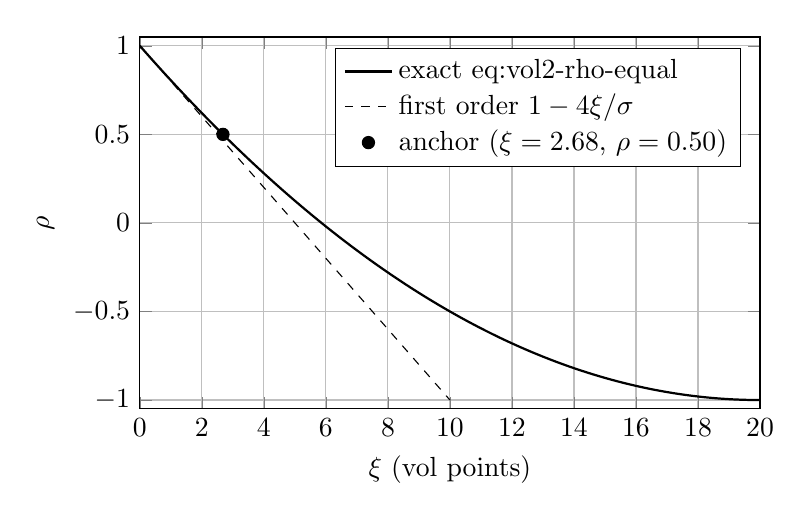
\begin{tikzpicture}
\begin{axis}[
  width=0.78\textwidth,
  height=0.52\textwidth,
  xlabel={$\xi$ (vol points)},
  ylabel={$\rho$},
  xmin=0, xmax=20,
  ymin=-1.05, ymax=1.05,
  grid=major,
  legend pos=north east,
  legend cell align=left,
]
% Exact: rho = 1 - 4 xi/sigma + 2 xi^2/sigma^2, sigma = 0.20, xi in vol points
\addplot[domain=0:20, samples=101, thick]
  {1 - 0.2*x + 0.005*x^2};
\addlegendentry{exact \eqref{eq:vol2-rho-equal}}
% First order: rho = 1 - 4 xi/sigma
\addplot[domain=0:10, samples=2, dashed]
  {1 - 0.2*x};
\addlegendentry{first order $1 - 4\xi/\sigma$}
\addplot[only marks, mark=*, mark size=2.2pt]
  coordinates {(2.6795, 0.5)};
\addlegendentry{anchor ($\xi = 2.68$, $\rho = 0.50$)}
\end{axis}
\end{tikzpicture}
\caption{The exact correlation--volatility relation
\eqref{eq:vol2-rho-equal} at equal vols $\sigma_1 = \sigma_2 = 20\%$. The
map runs from $\rho = 1$ at $\xi = 0$ down to $\rho = -1$ at
$\xi = \sigma = 20$ points --- exactly the two-name rungs of
Proposition~\ref{prop:vol2-rungs}. The dashed first-order line
$1 - 4\xi/\sigma$ is tangent at $\rho = 1$ and overstates $1-\rho$ away
from it; at the anchor point of Example~\ref{ex:vol2-anchor} the gap is
already visible. The map is convex in $\xi$: each further point of spread
costs less correlation than the last.}
\label{fig:vol2-rho-of-xi}
\end{figure}

The relation \eqref{eq:vol2-rho-exact} makes $\rho$ a determined function of
the vols once $\xi$ is held fixed. Its partial derivatives at fixed $\xi$
are the channel through which every vol move touches correlation.

\begin{proposition}[Vol sensitivities of $\rho$ at fixed spread]
\label{prop:vol2-rho-partials}
Differentiating \eqref{eq:vol2-rho-exact} at fixed $\xi$,
\begin{equation}
\boxed{\;
\atfixed{\pd{\rho}{\sigma_1}}{\xi}
 = \frac{2\xi}{\sigma_1^2}\Bigl(1 - \frac{\xi}{\sigma_2}\Bigr),
\qquad
\atfixed{\pd{\rho}{\sigma_2}}{\xi}
 = \frac{2\xi}{\sigma_2^2}\Bigl(1 - \frac{\xi}{\sigma_1}\Bigr).
\;}
\label{eq:vol2-rho-partials}
\end{equation}
In the equal-vol case $\sigma_1 = \sigma_2 = \sigma$, a parallel move
$\dd\sigma_1 = \dd\sigma_2 = \dd\sigma$ gives the total
\begin{equation}
\boxed{\;
\atfixed{\td{\rho}{\sigma}}{\xi}
 = \frac{4\xi}{\sigma^2} - \frac{4\xi^2}{\sigma^3}
 = \frac{4\xi}{\sigma^2}\Bigl(1 - \frac{\xi}{\sigma}\Bigr) \;>\; 0
\quad\text{for } 0 < \xi < \sigma,
\qquad\text{leading order: } +\frac{4\xi}{\sigma^2}.
\;}
\label{eq:vol2-drho-dsigma}
\end{equation}
The strict inequality holds on the open interval $0 < \xi < \sigma$
(equivalently $-1 < \rho < 1$) only: the slope vanishes at \emph{both}
rungs, $\xi = 0$ ($\rho = 1$) and $\xi = \sigma$ ($\rho = -1$).
\end{proposition}

\begin{proof}
Differentiate \eqref{eq:vol2-rho-exact} term by term in $\sigma_1$ at fixed
$\xi$: $+2\xi/\sigma_1^2 - 2\xi^2/(\sigma_1^2\sigma_2)$, which factors as
stated; symmetrically for $\sigma_2$. Summing the two at
$\sigma_1 = \sigma_2 = \sigma$ gives \eqref{eq:vol2-drho-dsigma}.
\end{proof}

\begin{remark}[Sign and degeneracy]
\label{rem:vol2-sign}
The sign in \eqref{eq:vol2-drho-dsigma} is \emph{positive} throughout the
interior of the ladder: with the spread fixed, raising $\sigma$ shrinks the
relative gap $1-\rho \approx 4\xi/\sigma$, pushing $\rho$ toward $1$. The
slope degenerates at both ends. At the top rung $\xi = 0$ ($\rho = 1$) the
factor $4\xi/\sigma^2$ vanishes: a perfectly correlated pair stays
perfectly correlated under fixed-$\xi$ re-marks, and anything that divides
by the slope \eqref{eq:vol2-drho-dsigma} --- as the shadow-Greek
constructions of the next chapter do --- must be guarded there. At the
bottom rung the picture depends on the vols. In general
$\atfixed{\partial\rho/\partial\sigma_1}{\xi} > 0$ if and only if
$\xi < \sigma_2$, which holds throughout the interior of the ladder
\eqref{eq:vol2-rungs} \emph{including} the bottom rung when
$\sigma_1 < \sigma_2$ (there $\xi = \sigma_1 < \sigma_2$, and the
$\sigma_1$-sensitivity stays strictly positive; it is the partial with
respect to the \emph{higher}-vol name, $\atfixed{\partial\rho/\partial
\sigma_2}{\xi} \propto (1 - \xi/\sigma_1)$, that dies). Only in the
equal-vol case do both partials vanish at the bottom rung: there
$\xi \to \sigma = \sigma_2$ and the factor $(1 - \xi/\sigma_2)$ kills the
sensitivity --- near $\rho = -1$ a re-mark of the spread no longer moves
correlation through the vols. The positive slope
\eqref{eq:vol2-drho-dsigma} is the single quantity the shadow Greeks of the
next chapter are built from.
\end{remark}

\section{Cega: the correlation sensitivity}
\label{sec:vol2-cega}

The value sensitivity to correlation is expressed through the position's
basket vega --- when the basket vol is the book's only correlation channel.
Let $V$ be the value of a correlation-sensitive book, viewed as a function
of $\rho$ with everything else held fixed. Differentiating
\eqref{eq:vol2-basket-identity},
\begin{equation}
\pd{\sB}{\rho} \;=\; \frac{\sigma_1\sigma_2}{4\sB} \;>\; 0,
\label{eq:vol2-dsB-drho}
\end{equation}
so, \emph{for a book whose only $\rho$-dependence is through $\sB$ ---
basket-vol instruments only, no spread or exchange legs} --- a position with
basket vol sensitivity $\pd{V}{\sB}$ (whose quoted vega is
$\VB = \tfrac1{100}\pd{V}{\sB}$) has
\begin{equation}
\pd{V}{\rho} \;=\; \pd{V}{\sB}\,\pd{\sB}{\rho}
             \;=\; \pd{V}{\sB}\,\frac{\sigma_1\sigma_2}{4\sB}.
\label{eq:vol2-dV-drho}
\end{equation}
The hypothesis matters. The chapter itself supplies the second channel: by
Lemma~\ref{lem:vol2-pythagoras}, the Margrabe vol
$\SigmaM = \sqrt{\sigma_1^2 + \sigma_2^2 - 2\rho\sigma_1\sigma_2}$ also
depends on $\rho$, with
$\pd{\SigmaM}{\rho} = -\sigma_1\sigma_2/\SigmaM$ (differentiate the
definition of $\SigmaM^2$) --- \emph{opposite} in sign to
\eqref{eq:vol2-dsB-drho}. For a general two-name book
$V(\sB(\rho), \SigmaM(\rho))$, carrying both basket-vol and spread legs,
the full chain rule is
\begin{equation}
\pd{V}{\rho}
 \;=\; \pd{V}{\sB}\,\frac{\sigma_1\sigma_2}{4\sB}
 \;-\; \pd{V}{\SigmaM}\,\frac{\sigma_1\sigma_2}{\SigmaM}.
\label{eq:vol2-dV-drho-full}
\end{equation}
The spread book of the exchange-option chapter lives in the second channel;
\eqref{eq:vol2-dV-drho} must never be applied to it.

\begin{remark}[The $\rho$-to-vol translation is singular at the bottom rung]
\label{rem:vol2-dsB-blowup}
Equation \eqref{eq:vol2-dsB-drho} \emph{diverges} as $\sB \to 0$ --- at
equal vols, as $\rho \to -1$, the bottom rung of
Proposition~\ref{prop:vol2-rungs}, where
$\sB = \tfrac12\abs{\sigma_1 - \sigma_2} = 0$. At equal vols
$\sB = \sigma\sqrt{(1+\rho)/2}$, so
$\pd{\sB}{\rho} = \tfrac14\sigma\sqrt{2/(1+\rho)}$: a blow-up of order
$(1+\rho)^{-1/2}$. On the running example's own line ($\sigma = 20\%$) the
mark is $0.0577$ at the anchor $\rho = 0.50$, $0.224$ at $\rho = -0.90$,
and $0.707$ at $\rho = -0.99$ --- twelve times the anchor. A book marked
near the PSD boundary therefore shows a finite $\pd{V}{\rho}$ but an
unbounded correlation-to-vol conversion: every $\Cega$-to-vega number in
this section is valid only bounded away from the bottom rung, and in a
decorrelation crisis it is the \emph{translation}, not necessarily the
risk, that explodes first. This is the mirror image of
Remark~\ref{rem:vol2-sign}, where the fixed-$\xi$ slope
$\atfixed{\dd\rho/\dd\sigma}{\xi}$ \emph{vanishes} at the same rung.
\end{remark}

\begin{definition}[$\Cega$]
\label{def:vol2-cega}
$\Cega$ is the correlation sensitivity quoted \emph{per correlation point}
(the ratified convention of the notation contract):
\begin{equation}
\boxed{\;
\Cega \;:=\; \frac{1}{100}\,\pd{V}{\rho},
\;}
\label{eq:vol2-cega}
\end{equation}
the P\&L of an absolute $+0.01$ move in $\rho$, exact by definition. For a
basket-only book, \eqref{eq:vol2-dV-drho} gives the desk form
$\Cega = \VB\,\dfrac{\sigma_1\sigma_2}{4\sB}$, with
$\VB = \tfrac1{100}\pd{V}{\sB}$ the basket vega per vol point: the two
normalisers ($/100$ on each side) cancel against each other.
\end{definition}

\begin{definition}[Gap-bump P\&L $\Delta V_{\omega}$ --- local to this
chapter]
\label{def:vol2-gapbump}
The \emph{gap-bump P\&L} is the exact value change under the convex bump
$\rho^{*} = \rho + (1-\rho)/10$ of the conventions list:
\begin{equation}
\Delta V_{\omega} \;:=\; V(\rho^{*}) - V(\rho).
\label{eq:vol2-gapbump}
\end{equation}
It is a distinct object from $\Cega$, and this volume never uses the bare
ratified symbol $\Cega$ for it; the routed-sensitivities chapter quotes
this same object under the locally scoped, subscripted desk name
$\Cega_{\mathrm{gap}}$, with the conversion to the ratified per-point
$\Cega$ stated there. To first order in the bump size,
\begin{equation}
\Delta V_{\omega}
 \;=\; \pd{V}{\rho}\,\frac{1-\rho}{10}
 \;+\; O\!\left(\Bigl(\frac{1-\rho}{10}\Bigr)^{\!2}\pdd{V}{\rho}\right)
 \;=\; 10\,(1-\rho)\,\Cega
 \;+\; O\!\left(\Bigl(\frac{1-\rho}{10}\Bigr)^{\!2}\pdd{V}{\rho}\right).
\label{eq:vol2-gapbump-linear}
\end{equation}
\end{definition}

\begin{remark}[Reconciling the two quotes]
\label{rem:vol2-cega-quotes}
Two quotes circulate on desks. The ratified symbol $\Cega$ is the
per-correlation-point quote of Definition~\ref{def:vol2-cega}; the gap-bump
P\&L $\Delta V_{\omega}$ is a desk convention for a finite, convex move
toward $\rho = 1$. The first-order conversion
$\Delta V_{\omega} \approx 10(1-\rho)\,\Cega$ carries a factor $10(1-\rho)$
--- equal to $5$ at $\rho = 0.50$ --- so the two are never interchangeable
without it. Three cautions. (i) The bump is \emph{one-sided}, always toward
$\rho = 1$: it never measures the decorrelation tail the dispersion desk
actually fears, and for a convexity-carrying correlation book it
understates that tail; a symmetric $\pm$ bump pair is the honest convexity
quote. (ii) The linearisation error
$O\bigl(((1-\rho)/10)^2\,\partial^2 V/\partial\rho^2\bigr)$ in
\eqref{eq:vol2-gapbump-linear} grows toward low $\rho$, where the bump is
largest ($(1-\rho)/10 = 0.2$ at $\rho = -1$) and where
$\pd{\sB}{\rho}$ varies fastest (Remark~\ref{rem:vol2-dsB-blowup}).
(iii) Inverting \eqref{eq:vol2-gapbump-linear} as
$\pd{V}{\rho} \approx 10\,\Delta V_{\omega}/(1-\rho)$ is exact only to
first order in the bump; the exact per-point object is
$\pd{V}{\rho} = 100\,\Cega$, by definition. Whenever a number travels
between chapters it travels as $\Cega$, on the contract basis.
\end{remark}

\begin{remark}[Who is long, who is short]
\label{rem:vol2-cega-sign}
By \eqref{eq:vol2-dsB-drho}, anything long basket vol is long correlation: a
long basket (or index) straddle has $\pd{V}{\sB} > 0$ and hence
$\Cega > 0$. The dispersion package of Section~\ref{sec:vol2-cvc} --- long
single-name vol, short basket vol --- has $\Cega < 0$: it collects the CVC
spread and pays out when the names decorrelate. $\Cega$ is the desk's
scorecard for that side.
\end{remark}

\section{Two re-marking conventions: \stickyrho{} and \stickycvc}
\label{sec:vol2-sticky}

The identity \eqref{eq:vol2-basket-identity} is one equation in the four
quantities $(\sigma_1, \sigma_2, \rho, \sB)$; equivalently, by
\eqref{eq:vol2-rho-exact}, in $(\sigma_1, \sigma_2, \rho, \xi)$. A quote set
pins them at one instant, but when the single-name vols move the desk must
decide what its marks \emph{do}. Two conventions reproduce the current
$\sB$ and differ only in their dynamics.

\begin{definition}[\stickyrho]
\label{def:vol2-stickyrho}
Under \stickyrho, correlation is held fixed as vols move: $\dd\rho = 0$,
and $\xi$ floats. The basket vol moves only through the vol arguments of
\eqref{eq:vol2-basket-identity}:
\begin{equation}
\dd\sB \;=\; \atfixed{\pd{\sB}{\sigma_1}}{\rho}\dd\sigma_1
        + \atfixed{\pd{\sB}{\sigma_2}}{\rho}\dd\sigma_2,
\qquad
\atfixed{\pd{\sB}{\sigma_i}}{\rho}
 = \frac{\sigma_i + \rho\,\sigma_j}{4\sB},\quad j \ne i.
\label{eq:vol2-stickyrho-dsB}
\end{equation}
(The partial follows in one line from \eqref{eq:vol2-basket-identity}
squared: $2\sB\,\atfixed{\partial\sB/\partial\sigma_i}{\rho} =
\tfrac12\sigma_i + \tfrac12\rho\,\sigma_j$ at fixed $\rho$.)
\end{definition}

\begin{definition}[\stickycvc]
\label{def:vol2-stickycvc}
Under \stickycvc, the CVC spread --- equivalently, by
Proposition~\ref{prop:vol2-cvc-xi}, the basket vol spread $\xi$ at fixed
spot and expiry --- is held invariant: $\dd\xi = 0$. The basket vol is
pinned to the single-name average minus a fixed gap and $\rho$ becomes the
determined function $\rho(\sigma_1, \sigma_2, \xi)$ of
\eqref{eq:vol2-rho-exact}:
\begin{equation}
\sB = \tfrac12(\sigma_1 + \sigma_2) - \xi,
\qquad
\dd\sB = \tfrac12\,\dd\sigma_1 + \tfrac12\,\dd\sigma_2,
\qquad
\dd\rho = \atfixed{\pd{\rho}{\sigma_1}}{\xi}\dd\sigma_1
        + \atfixed{\pd{\rho}{\sigma_2}}{\xi}\dd\sigma_2 .
\label{eq:vol2-stickycvc-dsB}
\end{equation}
\end{definition}

\begin{remark}[The pair is exhaustive here, and the difference is the risk]
\label{rem:vol2-sticky-pair}
For this corpus the two conventions are the whole menu: the shadow Greeks
of the next chapter are exactly the difference between the \stickycvc{} and
\stickyrho{} values of the corresponding total Greek, and they vanish
identically under \stickyrho{} (with $\dd\rho = 0$ the correlation channel
carries nothing). The choice between the two is the model risk of the
two-name book: same marks today, different P\&L tomorrow.
\end{remark}

The size of that difference is visible already at first order. Take the
anchor marks of Example~\ref{ex:vol2-anchor} ($\sigma_1 = \sigma_2 = 20\%$,
$\rho = 0.50$) and bump both single-name vols by $+1$ vol point. Under
\stickycvc, \eqref{eq:vol2-stickycvc-dsB} moves the basket vol one for one:
$\dd\sB = +1.00$ point. Under \stickyrho, \eqref{eq:vol2-stickyrho-dsB}
gives, at equal vols,
$\atfixed{\dd\sB/\dd\sigma}{\rho} = \sigma(1+\rho)/(2\sB) = \sB/\sigma
 = \sqrt{(1+\rho)/2} = 0.866$,
so $\dd\sB = +0.87$ points. The missing $0.13$ points of basket vol is what
the \stickycvc{} correlation re-mark supplies (correlation rises per
\eqref{eq:vol2-drho-dsigma}), and $0.13$ points of basket vega P\&L on
every parallel vol move is precisely the kind of risk the direct Greeks at
fixed $\rho$ never show. Quantifying it is the business of the shadow
Greeks.

\section{The anchor example}
\label{sec:vol2-anchor}

\begin{example}[Anchor numbers --- the running example of
Chapters~1--3]
\label{ex:vol2-anchor}
Take $\sigma_1 = \sigma_2 = \sigma = 20\%$ and $\rho = 0.50$, expiry
$T = 1$, and a book marked at $\Cega = +0.2$ per correlation point
(Definition~\ref{def:vol2-cega}). The correlation mark is the whole
threaded declaration: Chapters~2--3 consume $\pd{V}{\rho} = 20$ and the
channel slope computed below, nothing else --- the routed-sensitivities
chapter re-declares the same mark as the differential parameter of its
declared book class, a book carried through its correlation channel
alone. For the vega translation of this section --- and only there ---
read the mark through a \emph{hypothetical basket-only carrier} (sole
correlation channel $\sB$, e.g.\ net long the basket straddle against
single-name vol), so that \eqref{eq:vol2-dV-drho} applies to it.

\emph{Basket vol and spread.} Exactly,
$\sB = 0.20\sqrt{\tfrac12(1+0.5)} = 0.20\sqrt{0.75} = 0.17321$ and
$\xi = 0.20 - 0.17321 = 0.02679$ ($2.68$ vol points). The first-order
$\xi \approx \sigma(1-\rho)/4 = 0.20 \times 0.50/4 = 0.025$ ($2.5$ points)
is within $7\%$ of exact and serves for estimates; the exact
$\xi = 0.02679$ is used for the book.

\emph{Consistency check against \eqref{eq:vol2-rho-exact}.} At
$\xi = 0.02679$: $\rho = 1 - 4(0.02679)/0.20 + 2(0.02679)^2/0.20^2
= 1 - 0.5358 + 0.0359 = 0.500$. The relation closes.

\emph{CVC spread.} At $S = 100$ (with $F = S$ under zero rates, flagged),
$\Pi \approx S\sqrt{T}\,\xi/\sqrt{2\pi} = 100 \times 0.3989 \times 0.02679
\approx 1.07$ per $100$ of basket notional
(Remark~\ref{rem:vol2-dispersion-price}); exact Black--Scholes under the
geometric convention $C_B = C(S_B, \sB)$ gives $1.06$, and the true
arithmetic-basket price is within a cent of that
(Lemma~\ref{lem:vol2-geo-bridge}).

\emph{Correlation sensitivities.} From \eqref{eq:vol2-dsB-drho},
$\pd{\sB}{\rho} = \sigma^2/(4\sB) = 0.04/0.69282 = 0.05774$: one full unit
of $\rho$ is worth $5.77$ basket vol points, so one correlation point
($+0.01$) moves $\sB$ by $0.058$ points. By
Definition~\ref{def:vol2-cega}, exactly,
\[
\pd{V}{\rho} \;=\; 100\,\Cega \;=\; 20,
\qquad
\pd{V}{\sB} \;=\; \pd{V}{\rho}\Big/\pd{\sB}{\rho}
 = \frac{20}{0.05774} = 346.4,
\qquad
\VB = +3.46
\]
per vol point --- the second step is \eqref{eq:vol2-dV-drho}, legitimate
for the basket-only carrier and for it alone; the number is this
section's translation illustration, not a threaded mark, and no worked
number in Chapters~2--3 consumes it. A \emph{basket-only} book carrying
$\Cega = +0.2$ at these marks is implicitly long about $3\tfrac12$ basket
vega points. Under the desk's gap bump ($\rho^{*} = 0.55$),
\eqref{eq:vol2-gapbump-linear} gives
$\Delta V_{\omega} \approx 10\,(1-\rho)\,\Cega = +1$ --- first order in
the bump size; any convexity $\partial^2 V/\partial\rho^2$ the book
carries is not in this number.

\emph{The channel slope.} From \eqref{eq:vol2-drho-dsigma},
\[
\atfixed{\td{\rho}{\sigma}}{\xi}
 = \frac{4(0.02679)(0.20 - 0.02679)}{0.20^3}
 = \frac{4 \times 0.02679 \times 0.17321}{0.008}
 = +2.321 :
\]
under \stickycvc, a $+1$ vol-point parallel move in the single names
re-marks correlation by $+2.3$ correlation points. This slope, consumed
against $\pd{V}{\rho} = 20$, is the input to the shadow vega and shadow
delta of the next chapter; the same anchor reappears in the exchange-option
chapter, where Lemma~\ref{lem:vol2-pythagoras} gives the companion Margrabe
vol $\SigmaM = \sigma\sqrt{2(1-\rho)} = 0.20$ at $\rho = 0.50$.
\end{example}

\begin{table}[htbp]
\centering
\begin{tabular}{@{}llrl@{}}
\toprule
Quantity & Source & Anchor value & Units / basis \\
\midrule
$\sigma_1 = \sigma_2 = \sigma$ & given & $20\%$ & vol (absolute $0.20$) \\
$\rho$ & given & $0.50$ & pure number \\
$\sB$ & \eqref{eq:vol2-basket-identity} & $17.32$ & vol points \\
$\xi$ exact (first order) & \eqref{eq:vol2-xi}, Thm~\ref{thm:vol2-first-order-xi} & $2.68$ ($2.50$) & vol points \\
$\Pi$ at $S = 100$, $T = 1$ & \eqref{eq:vol2-cvc-xi} & $\approx 1.07$ & per $100$ notional \\
$\pd{\sB}{\rho}$ & \eqref{eq:vol2-dsB-drho} & $0.0577$ & abs.\ vol per unit $\rho$ ($0.058$ pts / corr pt) \\
$\Cega$ & given & $+0.2$ & per correlation point (contract basis) \\
$\pd{V}{\rho} = 100\,\Cega$ & \eqref{eq:vol2-cega} & $20$ & per unit $\rho$ \\
$\Delta V_{\omega}$ & \eqref{eq:vol2-gapbump-linear} & $+1$ & gap bump $(1-\rho)/10$; first order \\
$\VB$ & \eqref{eq:vol2-dV-drho} & $+3.46$ & per vol point (basket-only carrier; illustration, not threaded) \\
$\atfixed{\dd\rho/\dd\sigma}{\xi}$ & \eqref{eq:vol2-drho-dsigma} & $+2.321$ & unit $\rho$ per unit $\sigma$ ($= 2.32$ corr pts / vol pt) \\
$\SigmaM$ & Lemma~\ref{lem:vol2-pythagoras} & $20\%$ & vol (absolute $0.20$) \\
\bottomrule
\end{tabular}
\caption{The anchor example, carried forward. Chapters~2 and~3 reuse these
numbers on the stated bases: the routed-sensitivities chapter builds
$\shvega$ and $\shdelta$ from
$\pd{V}{\rho} = 100\,\Cega = 20$ and the channel slope $+2.321$ --- the
correlation mark and the map, the only rows the thread consumes; its
declared book carries the mark through the correlation channel alone. The
$\VB$ row is the basket-only translation of Section~\ref{sec:vol2-cega},
an illustration Chapters~2--3 do not consume. The exchange-option
chapter prices the spread book at $\SigmaM = 20\%$ against the same
correlation mark, but computes that book's own $\pd{V}{\rho}$ through the
$\SigmaM$ channel of \eqref{eq:vol2-dV-drho-full}; it must not consume the
basket book's $20$.}
\label{tab:vol2-anchor}
\end{table}

The chapter's yield is a small set of exact objects --- the identity
\eqref{eq:vol2-basket-identity}, the spread \eqref{eq:vol2-xi} with its
ladder \eqref{eq:vol2-rungs}, the relation \eqref{eq:vol2-rho-exact} with
its fixed-$\xi$ slopes \eqref{eq:vol2-rho-partials}, and the $\Cega$
normalisation \eqref{eq:vol2-cega} --- plus one modelling choice,
\stickyrho{} versus \stickycvc. The next chapter takes the choice
seriously: it routes vol and spot moves through
$\rho(\sigma_1, \sigma_2, \xi)$ and prices what the direct Greeks leave
out.
%% ============================================================================
%% frag_volII_ch2.tex -- Routed Sensitivities II: Shadow Greeks and the
%% Correlation Update Rule (Vol II, Chapter 2)
%% Author: THORP. Governed by NOTATION_CONTRACT.md; macros from build/preamble.tex.
%% Specializes the routed-derivative operator of Volume I, Chapter 3 through
%% the convention-completed-route hook: route (F_i, sigma_i, rho).
%% ============================================================================

%% Locally scoped symbol of this chapter: the gap-bump correlation quotation.
%% NOT the contract's ratified per-correlation-point \Cega; conversion stated
%% once in rem:sh2:cega-units. No FORMALIS amendment is claimed or needed.
\providecommand{\Cegagap}{\Cega_{\mathrm{gap}}}

\chapter{Routed Sensitivities II: Shadow Greeks and the Correlation Update Rule}
\label{ch:sh2}

A long basket (or index) straddle is \emph{long correlation}: the basket
volatility rises when the constituents correlate, so
$\pd{\sB}{\rho} > 0$ and the position gains as $\rho$ marks up. The
short-correlation side of the same trade is the dispersion book --- long
single-name volatility, short index volatility. Whichever side of it a desk
holds, the position carries a risk that the direct Greeks do not show: when
the single-name volatilities move, the implied correlation may be forced to
move with them by the market's quoting convention, and the value change
routed through that forced move is booked nowhere on a fixed-$\rho$ risk
report. This chapter derives those missing sensitivities --- the
\emph{shadow Greeks} --- and the finite re-marking rule that books them
consistently.

The machinery is not new. Volume~I, Chapter~3 states one routed-derivative
operator: for an ordered chain of $C^2$ intermediates over a driver, the
total first derivative is the gradient--velocity contraction and the total
second derivative is the Hessian--velocity--velocity plus
gradient--acceleration contraction, each intermediate's own total
derivatives supplied by the same formula one level down. A specialization
supplies exactly three items: the driver, the ordered links with their
partial derivatives, and the partial derivatives of the value function.
Volume~I, Chapter~3 supplied the list $(F, \sigma)$; this chapter supplies
$(F_i, \sigma_i, \rho)$ --- the same operator, one link deeper:
\[
  S \;\longrightarrow\; F \;\longrightarrow\; \sigma
    \;\longrightarrow\; \rho \;\longrightarrow\; V.
\]
Correlation is not a function of spot until a quoting convention closes the
system. The convention studied here, \stickycvc{}, declares the basket vol
spread invariant; the implicit function theorem then determines $\rho$ as a
$C^2$ function of the single-name volatilities, appending one live link to
the Volume~I route. Under the alternative convention, \stickyrho{}, the
appended link is inert and every result of this chapter collapses to the
Volume~I route name by name. The shadow Greeks are, by definition, the
difference between the two completed routes; the model risk of the chapter
is the choice between them, and the shadow Greeks are its price.

The standing assumption of the corpus holds throughout: zero rates
and zero dividends, the forward map carried generally as $F_i(S_i)$ and the
collapse $F_i = S_i$ flagged at every point of use. One worked example ---
$\sigma = 20\%$, $\rho = 0.50$, spread $\xi = 2.68$ vol points exact
($2.5$ at first order),
$\Cegagap = +1$, the book carried throughout as the constant-$\Cegagap$
class of Section~\ref{sec:sh2:shadow-gamma} (one book model, declared once,
used in every worked number) --- is threaded through the entire chapter so
that every number reconciles with every other.

%% ===========================================================================
\section{The two-name setting: basket volatility, the spread, and Cega}
\label{sec:sh2:setting}
%% ===========================================================================

Every symbol is fixed before it is used.

The basket object is Chapter~1's. The moment-matching basket volatility
$\sB$ of the equal-weight two-name basket $S_B = \tfrac12(S_1 + S_2)$ is
Definition~\ref{def:vol2-basket}, Eq.~\eqref{eq:vol2-basket-identity}:
\[
  \sB \;=\; \sqrt{\tfrac14 \sigma_1^2 + \tfrac14 \sigma_2^2
                  + \tfrac12 \rho\, \sigma_1 \sigma_2}.
\]
Equation \eqref{eq:vol2-basket-identity} is the ratified
\emph{moment-matching definition} of $\sB$, not the exact implied
volatility of the arithmetic basket $\tfrac12(S_1 + S_2)$, which is not
lognormal; the arithmetic-versus-lognormal gap is quantified in
Lemma~\ref{lem:sh2:moment-match} and absorbed by the error term of
Proposition~\ref{prop:sh2:cvc-xi}.

The constituent volatilities in \eqref{eq:vol2-basket-identity} are not free
symbols: per the bridging identity of the notation contract, they are the
single-name at-the-money volatilities,
\begin{equation}\label{eq:sh2:C1}
  \sigma_i \;\equiv\; \satmi{i}(\lFi{i}, T), \qquad i = 1, 2,
\end{equation}
evaluated at the current forward, where $\lFi{i} = \ln(F_i / \Frefi{i})$;
the per-name symbols $\lFi{i}$ and $\Frefi{i}$ are the ones ratified by the
contract's C1 note (the name index is the C1 note's, not a local extension
of this chapter). Every derivative taken through $\sigma_i$ in this chapter therefore
inherits the Volume~I surface dynamics --- in particular the per-name ATM
slope $\volslope_i = \pd{\satmi{i}}{\lFi{i}}$ --- through this identity.
This is the single load-bearing hypothesis of the chapter: the correlation
convention is a relation among \emph{at-the-money} volatilities, so the only
spot sensitivity that reaches $\rho$ travels through $\satmi{i}$.

The basket vol spread $\xi$ is that of Definition~\ref{def:vol2-xi}: with
$\sbmean = \tfrac12(\sigma_1 + \sigma_2)$ the maximal ($\rho = 1$) basket
vol of \eqref{eq:vol2-sbar}, the boxed \eqref{eq:vol2-xi} sets
$\xi := \sbmean - \sB \ge 0$ --- the diversification benefit of the
basket, in vol points.

\begin{remark}[No-arbitrage reading of $\xi \ge 0$]\label{rem:sh2:noarb}
$\xi \ge 0$ is the upper rung of the two-name no-arbitrage ladder,
Proposition~\ref{prop:vol2-rungs} \eqref{eq:vol2-rungs}: a basket cannot
be more volatile than the weighted average of its constituents, with
equality iff $\rho = 1$. Thus $\xi$ is a clean,
sign-definite ``how far from perfectly correlated'' coordinate, and it is
the natural state variable for the dynamics studied here. A mark that
implies $\xi < 0$ is a free-money flag, not a market view; the clamp in the
update rule of Section~\ref{sec:sh2:update} enforces the bound. The price
counterpart is exact for the \emph{arithmetic-basket} form of the spread:
with the basket leg priced as the arithmetic-basket call
$\E\bigl(\tfrac12(S_{1,T} + S_{2,T}) - S_B\bigr)^+$, payoff convexity
gives the model-free bound
$\tfrac12 C(S_1, \sigma_1) + \tfrac12 C(S_2, \sigma_2)
- \E\bigl(\tfrac12(S_{1,T} + S_{2,T}) - S_B\bigr)^+ \ge 0$ with no
expansion
(Proposition~\ref{prop:vol2-cvc-modelfree}; proof of
Proposition~\ref{prop:sh2:cvc-xi}). The spread $\Pi$ of
Definition~\ref{def:sh2:cvc} subtracts the moment-matched lognormal call
$C(S_B, \sB)$ instead, so it inherits non-negativity only up to the
moment-match error of Lemma~\ref{lem:sh2:moment-match}:
$\Pi \ge -O\bigl(S(\sigma\sqrt{T})^3\bigr)$, not an exact sign.
\end{remark}

\begin{definition}[CVC spread: basket of calls versus call on the basket]
\label{def:sh2:cvc}
Fix an expiry $T > 0$; under zero rates, let $C(S, \sigma)$ be the
at-the-money price (strike equal to the forward, which under zero rates is
$F = S$, flagged) of a European call on an underlying of level $S$ and
implied volatility $\sigma$. The \emph{CVC spread} is the price difference
between a basket of single-name at-the-money calls and the at-the-money
call on the basket,
\begin{equation}\label{eq:sh2:cvc-def}
  \Pi \;:=\; w_1\, C(S_1, \sigma_1) + w_2\, C(S_2, \sigma_2)
             - C(S_B, \sB).
\end{equation}
$\Pi$ is a locally scoped symbol of this chapter.
\end{definition}

\begin{lemma}[Moment matching absorbs the arithmetic/lognormal gap]
\label{lem:sh2:moment-match}
With equal spots $S_1 = S_2 = S$ and lognormal legs carrying the stated
vols and correlation, the at-the-money (strike equal to the common forward
$S$) call on the arithmetic basket $\tfrac12(S_1 + S_2)$ and the
Black--Scholes call $C(S, \sB)$ on a lognormal underlying of volatility
$\sB$ agree to $O\bigl(S(\sigma\sqrt{T})^3\bigr)$: both equal
$S \sB \sqrt{T}/\sqrt{2\pi} + O\bigl(S(\sigma\sqrt{T})^3\bigr)$.
\end{lemma}

\begin{proof}
For any underlying $B_T$ with forward $\E[B_T] = S$, the ATM call is
$\E(B_T - S)^+ = \tfrac12 \E\abs{B_T - S}$ (add and subtract
$\tfrac12 \E(B_T - S) = 0$). For the arithmetic basket
$B_T = \tfrac12(S_{1,T} + S_{2,T})$ with lognormal legs, the variance is
\[
  \Var(B_T)
  = \tfrac14 S^2 \bigl[(e^{\sigma_1^2 T} - 1) + (e^{\sigma_2^2 T} - 1)
    + 2(e^{\rho \sigma_1 \sigma_2 T} - 1)\bigr]
  = S^2 \sB^2 T\,\bigl(1 + O(\sigma^2 T)\bigr)
\]
by \eqref{eq:vol2-basket-identity}, and to the same relative order each leg
is $S(1 + \sigma_i \sqrt{T} Z_i)$ with $(Z_1, Z_2)$ jointly standard normal
at correlation $\rho$, so $B_T - S$ is Gaussian up to an
$O(\sigma^2 T)$-relative residual whose contribution to
$\E\abs{B_T - S}$ enters at the stated order. Hence
$\tfrac12 \E\abs{B_T - S}
= \tfrac12 \sqrt{2/\pi}\,\mathrm{sd}(B_T)\,(1 + O(\sigma^2 T))
= S \sB \sqrt{T}/\sqrt{2\pi} + O\bigl(S(\sigma\sqrt{T})^3\bigr)$. The
lognormal call $C(S, \sB)$ has the same expansion by the ATM Taylor
expansion in the proof of Proposition~\ref{prop:sh2:cvc-xi}.
\end{proof}

Pricing $C(S_B, \sB)$ in \eqref{eq:sh2:cvc-def} as a lognormal call on the
arithmetic level with the moment-matched vol is therefore legitimate
exactly to the order carried below --- this is the load-bearing step of the
CVC--$\xi$ equivalence, and it is an approximation with a stated order, not
an identity.

\begin{proposition}[The CVC spread equals the vol spread at leading order]
\label{prop:sh2:cvc-xi}
With equal weights $w_1 = w_2 = \tfrac12$ and equal spots
$S_1 = S_2 = S$ (hence $S_B = S$), the CVC spread \eqref{eq:sh2:cvc-def}
satisfies
\begin{equation}\label{eq:sh2:cvc-xi}
  \Pi \;=\; \frac{S \sqrt{T}}{\sqrt{2\pi}}\, \xi
        \;+\; O\bigl(S(\sigma\sqrt{T})^3\bigr),
        \qquad \sigma := \max(\sigma_1, \sigma_2),
\end{equation}
with $\xi$ the basket vol spread \eqref{eq:vol2-xi}. Consequently, at
fixed spot and expiry, $\Pi$ is constant if and only if $\xi$ is constant,
to this order. The leading term is non-negative since $\xi \ge 0$; the
exact model-free inequality holds for the arithmetic-basket form of the
spread (see the proof), while $\Pi$ itself is non-negative only up to the
$O\bigl(S(\sigma\sqrt{T})^3\bigr)$ moment-match error.
\end{proposition}

\begin{proof}
At the money (strike equal to the forward; under zero rates, $F = S$,
flagged) the Black--Scholes call price at implied volatility $\sigma$ is
\[
  C(S, \sigma)
  = S\bigl[\ncdf(\tfrac12 \sigma \sqrt{T}) - \ncdf(-\tfrac12 \sigma \sqrt{T})\bigr]
  = S\bigl[2 \ncdf(\tfrac12 \sigma \sqrt{T}) - 1\bigr],
\]
with $\ncdf$ the standard normal distribution function. Since
$\ncdf'(0) = \npdf(0) = 1/\sqrt{2\pi}$ and $\ncdf''(0) = 0$, the Taylor
expansion is $\ncdf(u) = \tfrac12 + u/\sqrt{2\pi} + O(u^3)$; with
$u = \tfrac12 \sigma \sqrt{T}$,
\[
  C(S, \sigma) = \frac{S \sigma \sqrt{T}}{\sqrt{2\pi}}
                 + O\bigl((\sigma\sqrt{T})^3\bigr) S.
\]
Substituting into \eqref{eq:sh2:cvc-def} with $w_1 = w_2 = \tfrac12$ and
$S_1 = S_2 = S_B = S$,
\[
  \Pi = \frac{S \sqrt{T}}{\sqrt{2\pi}}
        \Bigl[\tfrac12(\sigma_1 + \sigma_2) - \sB\Bigr] + O(\cdot)
      = \frac{S \sqrt{T}}{\sqrt{2\pi}}\, \xi + O(\cdot)
\]
by \eqref{eq:vol2-xi}, the identification of $C(S_B, \sB)$ with the
arithmetic-basket call being Lemma~\ref{lem:sh2:moment-match}, absorbed by
the same error term. For the sign: with all three strikes at the common
forward $S$, the payoffs satisfy
\[
  \bigl(\tfrac12(S_{1,T} + S_{2,T}) - S\bigr)^+
  \;\le\; \tfrac12 (S_{1,T} - S)^+ + \tfrac12 (S_{2,T} - S)^+
\]
pointwise, by convexity of $x \mapsto (x - K)^+$; taking expectations under
any joint law reproducing the marks gives, with no expansion,
\[
  \tfrac12 C(S, \sigma_1) + \tfrac12 C(S, \sigma_2)
  \;\ge\; \E\bigl(\tfrac12(S_{1,T} + S_{2,T}) - S\bigr)^+ .
\]
This is exact model-free non-negativity for the \emph{arithmetic-basket}
CVC spread, whose basket leg is the arithmetic-basket call. The spread
$\Pi$ of Definition~\ref{def:sh2:cvc} subtracts the moment-matched
lognormal call $C(S, \sB)$ instead, which equals the arithmetic-basket
call only to $O\bigl(S(\sigma\sqrt{T})^3\bigr)$
(Lemma~\ref{lem:sh2:moment-match}), and that difference is not
sign-pinned; hence for $\Pi$ as defined, convexity delivers only
$\Pi \ge -O\bigl(S(\sigma\sqrt{T})^3\bigr)$ --- for tiny $\xi$ the error
term can dominate the leading term. The exact sign statement lives in vol
space: $\xi \ge 0$ holds because $\rho \le 1$
(Definition~\ref{def:vol2-xi}), and the leading-order identity
\eqref{eq:sh2:cvc-xi} ties the price and vol sign statements together
only at that order.
\end{proof}

\subsection{Conventions used throughout}\label{sec:sh2:conventions}

\begin{itemize}[leftmargin=1.5em]
\item \textbf{Vol points.} Vols and the spread $\xi$ are quoted in vol
  points; $1$ vol point $= 0.01$. A per-unit-$\sigma$ derivative is divided
  by $100$ to express it \emph{per vol point}. This is the source of every
  ``$/100$''.
\item \textbf{Correlation bump (the ``$/10$'').} Correlation is bumped not
  by a fixed absolute amount but by a fixed fraction $\tfrac1{10}$ of its
  remaining distance to $1$:
  $\rho^{*} = \rho + (1 - \rho)/10$. This is a convex move toward $1$ (it
  can never leave $[-1, 1]$). The bump $(1 - \rho)/10$ is a fixed fraction
  of the remaining gap, not a $0.10$ absolute shift in $\rho$.
\item \textbf{Spot normaliser (dollar delta).} A spot derivative
  $\pd{V}{S}$ is put on a cash footing by multiplying by the spot level:
  the \emph{dollar delta} $S\,\pd{V}{S}$ is the cash value of the
  equivalent stock position, the value change for a unit relative move
  $\dd S / S = 1$. The P\&L of a $1\%$ move is this divided by $100$.
\item \textbf{ATM vol slope.} $\volslope = \pd{\satm}{\lF}$ is the slope
  of the at-the-money volatility in the forward log-level --- how the ATM
  vol moves as the forward moves. It is the slope of the \emph{one} ATM
  point as the forward moves, never the slope of the smile across strikes
  (that is $\pd{\ssm}{\mln}$, which plays no role in this chapter because
  the correlation convention sees only ATM vols, per \eqref{eq:sh2:C1}).
  For an equity surface $\volslope < 0$: forward down, ATM vol up. Under
  zero rates, $F = S$ (flagged), the forward log-level and log-spot move
  one for one, $\dd \lF = \dd \ln S$ at fixed $\Fref$, so the slope may be
  read against log-spot without adjustment. On a term-structure footing
  the slope steepens at short tenors, empirically roughly as $1/\sqrt{T}$
  --- a stylised fact quoted for orientation, not a derived property, and
  not used quantitatively here; the worked example keeps $T = 1$.
\item \textbf{Vega per vol point.} $\VB = \tfrac1{100} \pd{V}{\sB}$ is the
  basket vega per vol point. ``Shadow'' will always mean the extra piece
  routed through $\rho(\sigma)$, additive to and on the same normalised
  basis as the corresponding direct Greek: the shadow delta carries the
  spot normaliser $S$, the shadow vega the vol normaliser $1/100$. The one
  footing exception is the shadow gamma, which is the spot gradient of the
  \emph{dollar} shadow delta and sits one factor of $S$ away from the raw
  $\Gadj$; the explicit conversion is stated at
  Definition~\ref{def:sh2:shadow-gamma} and additivity is only ever
  claimed after converting.
\end{itemize}

\subsection{Correlation sensitivity: the Cega}\label{sec:sh2:cega}

The value sensitivity to correlation is quoted in two conventions: per
correlation point --- the contract's ratified $\Cega$ of
Definition~\ref{def:vol2-cega} --- and per gap bump, the desk quotation
this chapter works in under the locally scoped name $\Cegagap$
(Definition~\ref{def:sh2:cega}). Both are expressed here through the
position's basket vega, via Chapter~1's $\rho$-to-vol translation: by
\eqref{eq:vol2-dsB-drho}, $\pd{\sB}{\rho} = \sigma_1\sigma_2/(4\sB) > 0$,
and by the chain rule \eqref{eq:vol2-dV-drho} a position with basket vol
sensitivity $\pd{V}{\sB}$ (quoted vega $\VB = \tfrac1{100}\pd{V}{\sB}$)
has $\pd{V}{\rho} = 100\,\VB\,\sigma_1\sigma_2/(4\sB)$.
Equation \eqref{eq:vol2-dV-drho} presumes the book reaches $\rho$ only
through $\sB$: basket legs plus $\rho$-independent single-name legs. Books
with direct $\rho$ exposure not routed through $\sB$ --- spread and
exchange options, whose exercise variance carries $-2\rho\sigma_1\sigma_2$
--- are outside this chapter's book class and are treated in their own
chapter.

\begin{definition}[Gap-bump Cega (locally scoped)]\label{def:sh2:cega}
$\Cegagap$ is this chapter's desk quotation name for the gap-bump P\&L of
Chapter~1: $\Cegagap := \Delta V_{\omega} = V(\rho^{*}) - V(\rho)$ of
Definition~\ref{def:vol2-gapbump}, \eqref{eq:vol2-gapbump}, under the gap
bump $\rho^{*} = \rho + (1 - \rho)/10$. $\Cegagap$ is a locally scoped
symbol of this chapter. It is \emph{not}
the contract's ratified $\Cega$, which is quoted per correlation point;
the conversion between the two is stated once in
Remark~\ref{rem:sh2:cega-units}, and no redefinition of the ratified
symbol is made or implied. Wherever $\Cegagap$ and $\rho$ are marked, the
book's raw correlation slope is recovered as
\begin{equation}\label{eq:sh2:dVdrho-from-cega}
  \pd{V}{\rho} \;\approx\; \frac{10\, \Cegagap}{1 - \rho},
\end{equation}
with equality exact only for books linear in $\rho$ over the bump
(Remark~\ref{rem:sh2:cega-linear}).
\end{definition}

\begin{remark}[Units: the ratified $\Cega$ versus the local $\Cegagap$]
\label{rem:sh2:cega-units}
A \emph{correlation point} is $0.01$ of $\rho$; the contract's ratified
$\Cega$ is the per-correlation-point sensitivity,
$\Cega = \tfrac1{100}\pd{V}{\rho}$. The two quotations convert, to the
first order of \eqref{eq:vol2-gapbump-linear}, by
\begin{equation}\label{eq:sh2:cega-convert}
  \Cegagap \;\approx\; 10\,(1 - \rho)\, \Cega,
\end{equation}
stated once here and used wherever a per-point number is needed. The gap
bump $(1-\rho)/10$ at the chapter's anchor $\rho = 0.50$ is $0.05$, i.e.\
five correlation points, so $\Cegagap = +1$ there corresponds to
$\Cega = +0.2$ per correlation point. The gap-bump quotation is the desk
convention because it respects the boundary at $\rho = 1$: the same book
re-quoted at higher $\rho$ shows a smaller $\Cegagap$ even at unchanged
$\pd{V}{\rho}$, which is exactly how much re-marking room remains. Both
quotations appear on risk reports; this chapter works in $\Cegagap$
throughout and keeps the ratified per-point $\Cega$ untouched ---
re-ratifying the gap bump as the contract's $\Cega$ would require a
FORMALIS amendment, and none is claimed.
\end{remark}

\begin{remark}[When the recovery \eqref{eq:sh2:dVdrho-from-cega} is exact]
\label{rem:sh2:cega-linear}
Equation \eqref{eq:sh2:dVdrho-from-cega} inverts a finite bump into a
derivative, so it is exact only for books linear in $\rho$ over the bump.
For the constant-$\Cegagap$ class of
Section~\ref{sec:sh2:shadow-gamma} --- the book model of the worked
thread --- the identity $\pd{V}{\rho} = 10\,\Cegagap/(1 - \rho)$ is
adopted as the \emph{definition} of the class parameter $\Cegagap$ (the
differential quotation): for that book the finite gap-bump value differs
from the parameter by bump convexity,
$10 \ln(10/9) \approx 1.054$ per unit, a $\approx 5\%$ quotation nuance.
The threaded example declares $\Cegagap = +1$ as the differential
parameter, so every closed form below that uses
\eqref{eq:sh2:dVdrho-from-cega} as an identity does so under this
declaration, not by assuming the bump away.
\end{remark}

%% ===========================================================================
\section{The exact correlation--volatility relation}\label{sec:sh2:exact}
%% ===========================================================================

Everything downstream rests on one identity, established once in
Chapter~1 by solving \eqref{eq:vol2-basket-identity} for $\rho$ and
substituting the spread: the boxed exact relation of
Proposition~\ref{prop:vol2-exact-rho}, Eq.~\eqref{eq:vol2-rho-exact},
\[
  \rho \;=\; 1
  \;-\; 2\Bigl(\frac{1}{\sigma_1} + \frac{1}{\sigma_2}\Bigr)\xi
  \;+\; \frac{2 \xi^2}{\sigma_1 \sigma_2},
  \qquad \sB = \tfrac12(\sigma_1 + \sigma_2) - \xi .
\]

\begin{corollary}[Admissibility factorisation]\label{cor:sh2:admissible}
Equation \eqref{eq:vol2-rho-exact} factorises at both boundaries:
\begin{equation}\label{eq:sh2:admissible}
  1 - \rho \;=\; \frac{2\xi\,(\sigma_1 + \sigma_2 - \xi)}{\sigma_1 \sigma_2},
  \qquad
  1 + \rho \;=\; \frac{2\,(\sigma_1 - \xi)(\sigma_2 - \xi)}{\sigma_1 \sigma_2}.
\end{equation}
Consequently every admissible mark ($\sigma_i > 0$, $\rho \in [-1, 1]$)
satisfies
\begin{equation}\label{eq:sh2:xi-band}
  0 \;\le\; \xi \;\le\; \min(\sigma_1, \sigma_2),
\end{equation}
with $\xi = 0$ iff $\rho = 1$ and $\xi = \min(\sigma_1, \sigma_2)$ iff
$\rho = -1$: the sensitivity-degeneracy locus $\xi = \min(\sigma_1,
\sigma_2)$ of Proposition~\ref{prop:sh2:link} is exactly the $\rho = -1$
boundary.
\end{corollary}

\begin{proof}
Both identities in \eqref{eq:sh2:admissible} are one-line rearrangements
of \eqref{eq:vol2-rho-exact}. The band \eqref{eq:sh2:xi-band}, with its
attainment cases, is the $\xi$ form of the two-name rungs,
Proposition~\ref{prop:vol2-rungs} \eqref{eq:vol2-rungs}; it is not
re-proved here. Conversely, a $\xi$ inside the band produces
$\rho \in [-1, 1]$ by \eqref{eq:sh2:admissible}, since both numerators are
then non-negative.
\end{proof}

The equal-vol specialisation is Corollary~\ref{cor:vol2-equal-vol}: for
$\sigma_1 = \sigma_2 = \sigma$, \eqref{eq:vol2-rho-equal} gives the exact
$1 - \rho = 2\xi(2\sigma - \xi)/\sigma^2$, and at leading order in the
small quantity $\xi/\sigma$, $1 - \rho \approx 4\xi/\sigma$. The converse
first-order expansion of the spread is
Theorem~\ref{thm:vol2-first-order-xi}: expanding
\eqref{eq:vol2-basket-identity} about $1 - \rho = 0$
(Eq.~\eqref{eq:vol2-sB-expansion}) gives
$\xi = \tfrac14 \sigma (1 - \rho) + O((1 - \rho)^2)$ at equal vols and
$\xi \approx \tfrac12\, \sigma_1 \sigma_2 (1 - \rho)/(\sigma_1 + \sigma_2)$
for unequal vols.

\begin{remark}[Validity]\label{rem:sh2:validity}
Equation \eqref{eq:vol2-rho-exact} is exact for all
$(\sigma_1, \sigma_2, \xi)$ with $\sigma_i > 0$ and is the backbone of
everything below. The leading-order forms $1 - \rho \approx 4\xi/\sigma$
and $\xi \approx \sigma(1 - \rho)/4$ are equal-vol shortcuts valid near
$\rho \approx 1$ (small $\xi/\sigma$); they are used only for intuition and
quick estimates, never where the exact formula is needed. The worked
thread below quantifies the error at $\rho = 0.5$: about $7\%$ ---
acceptable for a limit check, not for a mark.
\end{remark}

\begin{example}[Anchor numbers for the threaded example]\label{ex:sh2:anchor}
$\sigma_1 = \sigma_2 = \sigma = 20\%$, $\rho = 0.50$, both names quoted at
their ATM points per \eqref{eq:sh2:C1}. Exactly,
$\sB = 0.20\sqrt{0.75} = 0.173205$ and
$\xi = 0.20 - 0.173205 = 0.026795$ ($2.68$ vol points). The first-order
$\xi \approx \sigma(1 - \rho)/4 = 0.20 \times 0.50 / 4 = 0.025$
($2.5$ points) is within $7\%$ of exact and serves for estimates; the
book carries the exact $\xi = 0.026795$. These numbers ($\sigma = 20\%$,
$\rho = 0.5$, exact $\xi = 2.68$ points, $\Cegagap = +1$) run through the whole
chapter.
\end{example}

\begin{figure}[ht]
\centering
\begin{tikzpicture}
\begin{axis}[
  width=0.86\textwidth, height=6.6cm,
  xlabel={$\sigma$ (both names, parallel)},
  ylabel={$\rho$},
  legend pos=south east,
  legend cell align=left,
  grid=major,
  domain=0.11:0.40, samples=160, no markers,
  ymin=0.0, ymax=1.0,
  every axis plot/.append style={thick}]
  \addplot[black]
    {1 - 4*0.026795/x + 2*0.026795^2/(x^2)};
  \addlegendentry{\stickycvc{}: exact $\rho(\sigma)$ at $\xi = 0.026795$}
  \addplot[black, dashed]
    {1 - 4*0.026795/x};
  \addlegendentry{leading order $1 - 4\xi/\sigma$}
  \addplot[black, dotted]
    {0.5};
  \addlegendentry{\stickyrho{}: $\rho$ held at $0.50$}
  \addplot[only marks, mark=*, mark size=1.8pt] coordinates {(0.20, 0.50)};
\end{axis}
\end{tikzpicture}
\caption{The correlation forced by the \stickycvc{} convention as both
single-name ATM vols move in parallel, at the frozen spread
$\xi = 0.026795$ of Example~\ref{ex:sh2:anchor} (dot: the anchor
$\sigma = 20\%$, $\rho = 0.50$). The exact map
\eqref{eq:vol2-rho-equal} (solid) is concave and increasing: vols up,
correlation up. The leading-order form (dashed) is accurate near
$\rho \approx 1$ and understates $\rho$ at the anchor by the $7\%$ of
Remark~\ref{rem:sh2:validity}. Under \stickyrho{} (dotted) correlation does
not respond at all; the vertical distance between the solid and dotted
curves is what the shadow Greeks of
Section~\ref{sec:sh2:shadow} price.}
\label{fig:sh2:rho-of-sigma}
\end{figure}

%% ===========================================================================
\section{Sticky-CVC as a convention-completed route}\label{sec:sh2:convention}
%% ===========================================================================

The convention is stated precisely --- in which variables the spread is
held fixed, under which moves, and with which consequence for $\rho$ ---
and identified as a convention-completed route in the sense of Volume~I,
Chapter~3.

\begin{assumption}[\stickycvc{}: the CVC spread is held constant]
\label{ass:sh2:sticky-cvc}
As the volatility surface moves, the CVC spread
(Definition~\ref{def:sh2:cvc}) is held \emph{invariant}; equivalently ---
to the leading order in $\sigma\sqrt{T}$ at which
Proposition~\ref{prop:sh2:cvc-xi} identifies the two --- at fixed spot and
expiry the basket vol spread
$\xi = \tfrac12(\sigma_1 + \sigma_2) - \sB$ is held invariant. What the
contract adopts as \stickycvc{}, and what everything below uses, is the
$\xi = \text{const}$ form; the identification with the traded option
spread $\Pi$ carries the $O((\sigma\sqrt{T})^3)$ caveat of
Proposition~\ref{prop:sh2:cvc-xi}. Concretely:
\begin{enumerate}[label=(\roman*)]
\item The state variables that move are the single-name ATM vols
  $(\sigma_1, \sigma_2)$ --- driven either directly (a vega shock) or
  indirectly by spot through the per-name ATM slopes $\volslope_i$
  (Section~\ref{sec:sh2:shadow}).
\item Under any such move, $\dd \xi = 0$.
\item Consequently the basket vol is pinned to the single-name average
  minus a fixed gap, and $\rho$ is a determined function of the vols:
  \begin{equation}\label{eq:sh2:pinned}
    \sB = \tfrac12(\sigma_1 + \sigma_2) - \xi,
    \qquad \xi = \text{const},
    \qquad \rho = \rho(\sigma_1, \sigma_2, \xi)
    \ \text{via \eqref{eq:vol2-rho-exact}}.
  \end{equation}
\end{enumerate}
\end{assumption}

\begin{remark}[The convention closes the route]\label{rem:sh2:completed-route}
This is precisely a quoting convention in the sense of the
convention-completed-route definition of Volume~I, Chapter~3: the invariant
is $g(\sigma_1, \sigma_2, \rho) = \sbmean - \sB(\sigma_1, \sigma_2, \rho)$,
and by \eqref{eq:vol2-dsB-drho},
\[
  \pd{g}{\rho} = -\pd{\sB}{\rho} = -\frac{\sigma_1 \sigma_2}{4 \sB} \neq 0,
\]
so the implicit function theorem determines
$\rho = \rho(\sigma_1, \sigma_2, \xi)$ locally as a $C^2$ function of the
vols --- here globally and in closed form, by
Proposition~\ref{prop:vol2-exact-rho}. The correlation is thereby appended
as one more link to the Volume~I route $S_i \to F_i \to \sigma_i$, and
every routed derivative of this chapter is an instance of the
routed-derivative operator of Volume~I, Chapter~3 applied to the completed
route $(F_i, \sigma_i, \rho)$. Under \stickyrho{} the invariant is $\rho$
itself, the appended link is inert, and the completed route collapses to
the Volume~I route name by name.
\end{remark}

\paragraph{What the convention implies for surface motion.}
Differentiate $\sB = \tfrac12(\sigma_1 + \sigma_2) - \xi$ with
$\dd \xi = 0$:
\begin{equation}\label{eq:sh2:dsB}
  \dd \sB = \tfrac12\, \dd \sigma_1 + \tfrac12\, \dd \sigma_2 .
\end{equation}
A parallel $+1$ vol-point shift $\dd\sigma_1 = \dd\sigma_2 = +0.01$ thus
raises $\sB$ by exactly $+0.01$. To keep $\xi$ fixed while $\sB$ tracks the
average, implied correlation must rise. The next proposition quantifies
this --- it is the live link derivative that the completed route transmits.

\begin{proposition}[The correlation link derivatives]\label{prop:sh2:link}
Under Assumption~\ref{ass:sh2:sticky-cvc}, the partial derivatives of
$\rho(\sigma_1, \sigma_2, \xi)$ at fixed $\xi$ are
\begin{equation}\label{eq:sh2:drho-dsigmai}
  \atfixed{\pd{\rho}{\sigma_1}}{\xi}
  = \frac{2\xi}{\sigma_1^2}\Bigl(1 - \frac{\xi}{\sigma_2}\Bigr),
  \qquad
  \atfixed{\pd{\rho}{\sigma_2}}{\xi}
  = \frac{2\xi}{\sigma_2^2}\Bigl(1 - \frac{\xi}{\sigma_1}\Bigr),
\end{equation}
each strictly positive for $0 < \xi < \sigma_j$ ($j$ the other name). In
the symmetric case $\sigma_1 = \sigma_2 = \sigma$ moving in parallel
($\dd\sigma_1 = \dd\sigma_2 = \dd\sigma$), the total slope is their sum,
\begin{equation}\label{eq:sh2:drho-dsigma}
  \atfixed{\td{\rho}{\sigma}}{\xi}
  = \frac{4\xi}{\sigma^2}\Bigl(1 - \frac{\xi}{\sigma}\Bigr)
  = \frac{4\xi(\sigma - \xi)}{\sigma^3} \;>\; 0,
  \qquad\text{leading order: } +\frac{4\xi}{\sigma^2}.
\end{equation}
\end{proposition}

\begin{proof}
Differentiate \eqref{eq:vol2-rho-exact} in $\sigma_1$ at fixed
$(\sigma_2, \xi)$:
\[
  \atfixed{\pd{\rho}{\sigma_1}}{\xi}
  = \frac{2\xi}{\sigma_1^2} - \frac{2\xi^2}{\sigma_1^2 \sigma_2}
  = \frac{2\xi}{\sigma_1^2}\Bigl(1 - \frac{\xi}{\sigma_2}\Bigr),
\]
and symmetrically in $\sigma_2$. Positivity is immediate from
$0 < \xi < \sigma_j$. For the symmetric parallel move set
$\sigma_1 = \sigma_2 = \sigma$ and sum the two partials; equivalently,
differentiate \eqref{eq:vol2-rho-equal} directly:
$\td{\rho}{\sigma} = 4\xi/\sigma^2 - 4\xi^2/\sigma^3$.
\end{proof}

\begin{remark}[Sign]\label{rem:sh2:sign}
The slope \eqref{eq:sh2:drho-dsigma} is \emph{positive}: with the spread
fixed, raising $\sigma$ shrinks the relative gap
$(1 - \rho) \approx 4\xi/\sigma$, pushing $\rho$ toward $1$. Intuitively,
$\xi$ is an absolute number of vol points; at a higher vol level the same
absolute diversification benefit is a smaller relative one, and a smaller
relative benefit means higher correlation. The degeneracy at
$\xi \to \sigma_j$ --- where the factor $(1 - \xi/\sigma_j)$ kills the
sensitivity --- is, by Corollary~\ref{cor:sh2:admissible}, the $\rho = -1$
admissibility boundary itself; it is picked up again in the boundary
conditions of Section~\ref{sec:sh2:update}.
\end{remark}

\begin{remark}[The two conventions, and what the difference costs]
\label{rem:sh2:two-conventions}
Two re-marking conventions reproduce the current $\sB$ and differ only in
their dynamics; one fixes $\rho$, the other fixes $\xi$, and the remaining
quantity moves:
\begin{itemize}[leftmargin=1.5em]
\item \stickyrho{}: $\dd\rho = 0$, $\xi$ varies. Then $\sB$ moves only
  through the vol terms in \eqref{eq:vol2-basket-identity} and the shadow
  Greeks of Section~\ref{sec:sh2:shadow} vanish identically.
\item \stickycvc{}: $\dd\xi = 0$, with $\rho$ determined by
  \eqref{eq:vol2-rho-exact}.
\end{itemize}
Per the hook of Volume~I, Chapter~3, the shadow Greeks are \emph{defined}
as the difference between the two completed routes; the pair is exhaustive
for this corpus, and the choice between them is the model risk of the
chapter. A desk that risk-manages under \stickyrho{} while the market
re-marks under \stickycvc{} will find the difference in its unexplained
P\&L --- that is where to look first when a vol move produces correlation
P\&L that the direct $\Cegagap$ bump did not predict.
\end{remark}

\begin{figure}[ht]
\centering
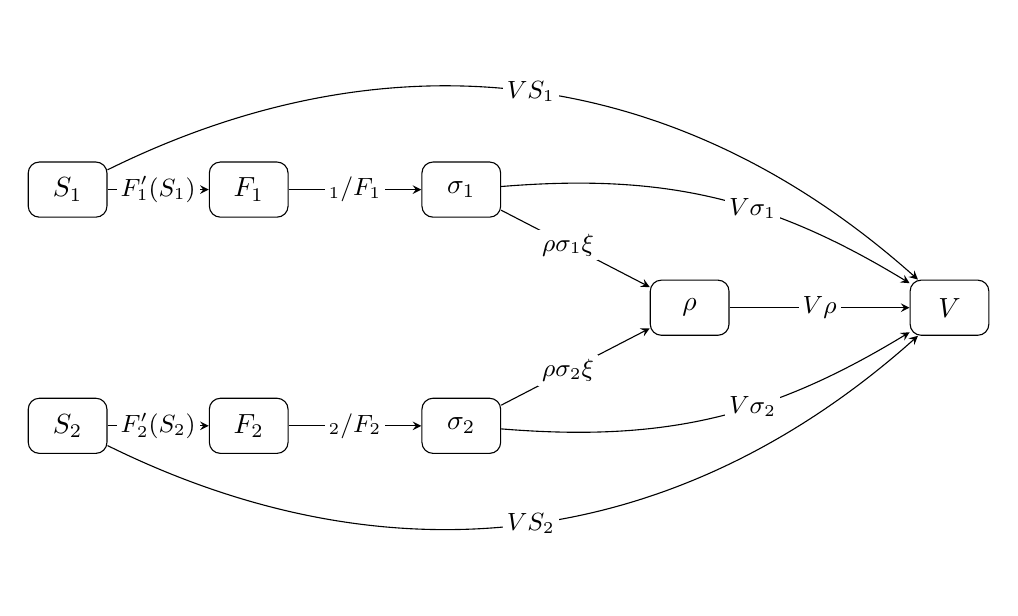
\begin{tikzpicture}[>=stealth,
  var/.style={draw, rounded corners, minimum height=7mm, minimum width=10mm,
              inner sep=2pt},
  lab/.style={font=\small, fill=white, inner sep=1.5pt}]
  \node[var] (S1)   at (0,1.5)   {$S_1$};
  \node[var] (S2)   at (0,-1.5)  {$S_2$};
  \node[var] (F1)   at (2.3,1.5) {$F_1$};
  \node[var] (F2)   at (2.3,-1.5){$F_2$};
  \node[var] (sig1) at (5.0,1.5) {$\sigma_1$};
  \node[var] (sig2) at (5.0,-1.5){$\sigma_2$};
  \node[var] (rho)  at (7.9,0)   {$\rho$};
  \node[var] (V)    at (11.2,0)  {$V$};
  \draw[->] (S1) -- node[lab]{$F_1'(S_1)$} (F1);
  \draw[->] (S2) -- node[lab]{$F_2'(S_2)$} (F2);
  \draw[->] (F1) -- node[lab]{$\volslope_1/F_1$} (sig1);
  \draw[->] (F2) -- node[lab]{$\volslope_2/F_2$} (sig2);
  \draw[->] (sig1) -- node[lab, pos=0.45]{$\atfixed{\pd{\rho}{\sigma_1}}{\xi}$} (rho);
  \draw[->] (sig2) -- node[lab, pos=0.45]{$\atfixed{\pd{\rho}{\sigma_2}}{\xi}$} (rho);
  \draw[->] (rho) -- node[lab]{$\pd{V}{\rho}$} (V);
  \draw[->] (sig1) to[bend left=18] node[lab, pos=0.6]{$\pd{V}{\sigma_1}$} (V);
  \draw[->] (sig2) to[bend right=18] node[lab, pos=0.6]{$\pd{V}{\sigma_2}$} (V);
  \draw[->] (S1) to[bend left=34] node[lab, pos=0.5]{$\pd{V}{S_1}$} (V);
  \draw[->] (S2) to[bend right=34] node[lab, pos=0.5]{$\pd{V}{S_2}$} (V);
\end{tikzpicture}
\caption{The convention-completed route of this chapter: the Volume~I
spot--volatility route, per name ($S_i \to F_i \to \sigma_i$, each
$\sigma_i \equiv \satmi{i}(\lFi{i}, T)$ per \eqref{eq:sh2:C1}, link
derivatives $\volslope_i / F_i$ through the forward), with the correlation
link appended by \stickycvc{} (Remark~\ref{rem:sh2:completed-route}). Under
zero rates, $F_i = S_i$ and $F_i'(S_i) = 1$ (flagged). Under \stickyrho{}
the two edges into $\rho$ transmit nothing and the diagram collapses to the
Volume~I route name by name. The direct edges $\pd{V}{S_i}$,
$\pd{V}{\sigma_i}$ carry the direct Greeks; the path through $\rho$ carries
the shadow Greeks.}
\label{fig:sh2:completed-route}
\end{figure}

%% ===========================================================================
\section{Shadow vega and shadow delta}\label{sec:sh2:shadow}
%% ===========================================================================

Once Assumption~\ref{ass:sh2:sticky-cvc} makes $\rho$ a function of the
vols, the direct Greeks --- direct delta $\pd{V}{S_i}$ and direct vega
$\pd{V}{\sB}$, both computed at fixed $\rho$ --- omit the value that moves
\emph{through} correlation. The omitted pieces are the terms
$\pd{V}{\rho} \cdot (\text{routed derivative of } \rho)$; these are the
shadow Greeks, and per the hook of Volume~I, Chapter~3 they are exactly the
difference between the \stickycvc{}- and \stickyrho{}-completed routes.

\subsection{Instantiating the interface}\label{sec:sh2:interface}

The routed-derivative operator of Volume~I, Chapter~3 requires three items
of a specialization:
\begin{enumerate}[label=(\alph*)]
\item \emph{Driver.} The spot $S_i$ of a given name (for the symmetric
  worked thread: a common level $S$ moving both names in parallel).
\item \emph{Ordered links.} $(F_i, \sigma_i, \rho)$:
  the forward $F_i(S_i)$ with derivative $F_i'(S_i)$; the single-name ATM
  vol $\sigma_i = \satmi{i}(\lFi{i}, T)$ with
  $\pd{\sigma_i}{F_i} = \volslope_i / F_i$ (the Volume~I moneyness link,
  specialised to the ATM point: the smile coordinate $\mln$ plays no role
  because the convention sees only ATM vols, per \eqref{eq:sh2:C1}); and
  the correlation $\rho(\sigma_1, \sigma_2, \xi)$ with link derivatives
  \eqref{eq:sh2:drho-dsigmai}.
\item \emph{Value partials.} $\pd{V}{\rho}$ from the book's marked
  $\Cegagap$ via \eqref{eq:sh2:dVdrho-from-cega} (under the declaration
  of Remark~\ref{rem:sh2:cega-linear}), alongside the direct
  $\pd{V}{S_i}$ and $\pd{V}{\sigma_i}$, which stay in their own (direct)
  buckets.
\end{enumerate}
The operator then outputs the routed correlation derivative
\begin{equation}\label{eq:sh2:drho-dS}
  \td{\rho}{S}
  \;=\; \sum_{i=1}^{2}
    \atfixed{\pd{\rho}{\sigma_i}}{\xi}\, \td{\sigma_i}{S},
  \qquad
  \td{\sigma_i}{S}
  \;=\; \frac{\volslope_i}{F_i}\, F_i'(S_i)\,\td{S_i}{S},
\end{equation}
the chain carried through the forward as always: the correlation link
composes with the forward links, it does not bypass them. Under zero rates,
$F_i = S_i$, so $F_i'(S_i) = 1$ and the factor collapses to
$\volslope_i / S_i$ (flagged). In the symmetric parallel thread
($S_1 = S_2 = S$, $\sigma_1 = \sigma_2 = \sigma$,
$\volslope_1 = \volslope_2 = \volslope$, $\td{S_i}{S} = 1$), the sum
\eqref{eq:sh2:drho-dS} collapses to
\begin{equation}\label{eq:sh2:drho-dS-symmetric}
  \td{\rho}{S}
  = \atfixed{\td{\rho}{\sigma}}{\xi} \cdot \frac{\volslope}{S}
  \qquad \text{(under zero rates, $F = S$, flagged),}
\end{equation}
with $\atfixed{\td{\rho}{\sigma}}{\xi}$ the parallel slope
\eqref{eq:sh2:drho-dsigma}.

\subsection{Shadow vega}\label{sec:sh2:shadow-vega}

\textbf{Bumped:} $\sigma$ ($+1$ vol point, both names in parallel).
\textbf{Held fixed:} the spread $\xi$
(Assumption~\ref{ass:sh2:sticky-cvc}), spot, time.
\textbf{Chain:} $\sigma \to \rho \to V$, via
\eqref{eq:sh2:drho-dsigma} then \eqref{eq:sh2:dVdrho-from-cega}.

\begin{definition}[Shadow vega]\label{def:sh2:shadow-vega}
The \emph{per-vol-point value change routed through correlation},
\begin{equation}\label{eq:sh2:shadow-vega-def}
  \shvega \;:=\; \frac{1}{100}\, \pd{V}{\rho}\,
                 \atfixed{\td{\rho}{\sigma}}{\xi}.
\end{equation}
This is the normalised first-order difference between the two completed
routes stated in the hook of Volume~I, Chapter~3, now with every factor
evaluable in closed form.
\end{definition}

\begin{proposition}[Shadow vega: exact and shortcut]\label{prop:sh2:shadow-vega}
In the equal-vol case, using
$\pd{V}{\rho} = 10\,\Cegagap/(1 - \rho)$ from
\eqref{eq:sh2:dVdrho-from-cega} (exact under the constant-$\Cegagap$
declaration of Remark~\ref{rem:sh2:cega-linear}) and the exact slope
$\atfixed{\td{\rho}{\sigma}}{\xi} = 4\xi(\sigma - \xi)/\sigma^3$ from
\eqref{eq:sh2:drho-dsigma},
\begin{equation}\label{eq:sh2:shadow-vega-exact}
  \shvega
  \;=\; \frac{1}{100} \cdot \frac{10\,\Cegagap}{1 - \rho}
        \cdot \frac{4\xi(\sigma - \xi)}{\sigma^3}
  \;>\; 0 \quad \text{for } \Cegagap > 0.
\end{equation}
At leading order in $\xi/\sigma$ this collapses to
\begin{equation}\label{eq:sh2:shadow-vega-shortcut}
  \shvega \;\approx\; +\frac{\Cegagap}{10\,\sigma}.
\end{equation}
\end{proposition}

\begin{proof}
Insert $\pd{V}{\rho}$ and $\atfixed{\td{\rho}{\sigma}}{\xi}$ into
\eqref{eq:sh2:shadow-vega-def} and apply the $1/100$ normaliser; that is
\eqref{eq:sh2:shadow-vega-exact}. For the shortcut replace
$1 - \rho \to 4\xi/\sigma$ and $\sigma - \xi \to \sigma$: the two factors
of $4\xi/\sigma$ cancel, leaving
$\td{V}{\sigma} \to 10\,\Cegagap/\sigma$ and
$\shvega \to \Cegagap/(10\sigma)$. The cancellation is \emph{leading order in
$\xi/\sigma$}, not exact: it uses the approximate $1 - \rho$ in the
denominator while the book's true $\pd{V}{\rho}$ uses the actual
$1 - \rho$.
\end{proof}

\textbf{Intuition.} Vol up $\Rightarrow$ (spread fixed) correlation up
$\Rightarrow$ a long-correlation book ($\Cegagap > 0$) gains. Hence the sign
is \emph{positive}: the book carries \emph{extra long vega} through the
correlation channel, additive to whatever direct (fixed-$\rho$) vega it
marks. For the threaded book the correlation channel is the whole
declaration --- the direct vega is a separate mark, not derivable from
$\Cegagap$, and is not restated in the thread. One caution on bases: the
one-for-one move \eqref{eq:sh2:dsB} is the \stickycvc{} \emph{total} and
already contains the correlation re-mark, so it must never be used to
state the direct term --- doing so double-counts the channel
(Example~\ref{ex:sh2:shadow-vega}).

\begin{example}[Shadow vega at the anchor]\label{ex:sh2:shadow-vega}
$\Cegagap = +1$, $\sigma = 20\%$, $\rho = 0.5$, $\xi = 0.026795$
(Example~\ref{ex:sh2:anchor}). The exact
\eqref{eq:sh2:shadow-vega-exact} uses the true gap $1 - \rho = 0.5$ and the
exact slope
\[
  \atfixed{\td{\rho}{\sigma}}{\xi}
  = \frac{4 (0.026795)(0.20 - 0.026795)}{0.20^3} = 2.321,
\]
giving
\[
  \shvega = \frac{1}{100} \cdot \frac{10}{0.5} \cdot 2.321
          = \frac{1}{100} \cdot 20 \cdot 2.321
          = +0.464 \ \text{per vol point}.
\]
The shortcut \eqref{eq:sh2:shadow-vega-shortcut} gives
$\Cegagap/(10\sigma) = 1/(10 \times 0.20) = +0.500$. The two differ by
$+0.036$ ($\approx 7.7\%$): the shortcut over-states because at
$\rho = 0.5$ the leading-order $4\xi/\sigma = 0.536$ exceeds the true
$1 - \rho = 0.50$; near $\rho \approx 1$ the gap closes. A $+1$ vol-point
parallel move thus adds about $+0.46$ of value through the correlation
channel, \emph{on top of} the direct vega in $\sB$.

For scale --- a hypothetical full re-mark, \emph{not} part of the
reconciling thread: the threaded book is declared through its correlation
channel alone, so it quotes no direct basket vega, and its per-vol-point
number for a parallel move \emph{is} the shadow vega. If instead the same
$\pd{V}{\rho} = 20$ were carried by the \emph{basket-only} carrier of
Chapter~1's translation illustration ($V$ a function of $\sB$ alone, a
book \emph{outside} this chapter's class per
Proposition~\ref{prop:sh2:shadow-gamma}), then
$\pd{\sB}{\rho} = \sigma_1\sigma_2/(4\sB) = 0.04/0.69282 = 0.05774$ would
translate the mark into a direct basket vega of
$\VB = \tfrac1{100}\,\pd{V}{\rho} \big/ \pd{\sB}{\rho}
     = \tfrac1{100} \times 20 / 0.05774 = 3.464$ per \emph{basket} vol
point. That book reconciles differently: at fixed $\rho$ a parallel
$+1$-point single-name move lifts $\sB$ by only
$\sqrt{(1+\rho)/2} = 0.866$ points (Chapter~1's \stickyrho{} partials),
direct P\&L $3.464 \times 0.866 = 3.00$; the correlation re-mark supplies
the missing $0.134$ basket points, worth $3.464 \times 0.134 = 0.46$ ---
the shadow vega again; and the \stickycvc{} total is
$3.00 + 0.46 = 3.46 = \VB \times 1$, the one-for-one move of
\eqref{eq:sh2:dsB}. Adding the shadow vega \emph{on top of} $\VB$ quoted
against that one-for-one move --- ``$3.464 + 0.464 = 3.93$'' --- would
double-count the channel, a $13\%$ over-statement of the vega and a
mis-sized hedge. No worked number in this chapter's thread is sourced
from the basket-only carrier.
\end{example}

\subsection{Shadow delta}\label{sec:sh2:shadow-delta}

The shadow vega routed a vol move into $\rho$; the shadow delta routes a
\emph{spot} move into $\rho$. The CVC invariant is a relation among
at-the-money vols, so $\rho$ is determined by the ATM single-name vols
through \eqref{eq:vol2-rho-exact}, and the only spot sensitivity that
reaches $\rho$ is the response of the ATM vol to the forward: the per-name
slope $\volslope_i = \pd{\satmi{i}}{\lFi{i}}$, transmitted through the
forward link as in \eqref{eq:sh2:drho-dS}. For an equity surface
$\volslope < 0$ --- forward down, ATM vol up.

\begin{remark}[The slope is an empirical input]\label{rem:sh2:slope-input}
$\volslope$ is the realised move of the ATM vol per unit of forward
log-level; it carries the entire spot-to-correlation channel. If the ATM
vol does not respond to the forward ($\volslope = 0$), the shadow delta
vanishes --- see the limits in Section~\ref{sec:sh2:coherence}. The
reference numerical engine of the corpus encodes exactly that convention
($\satm = \text{const}$, i.e.\ $\volslope = 0$): every shadow-delta and
shadow-gamma figure in this chapter is therefore \emph{invisible} to that
engine, and no worked number below is sourced from it; all are derived
analytically here under the stated $\volslope$.
\end{remark}

\textbf{Bumped:} spot $S$ (both names in parallel). \textbf{Held fixed:}
$\xi$. \textbf{Chain:}
$S \to F \to \sigma \to \rho \to V$, via $\volslope/F$, then
\eqref{eq:sh2:drho-dsigma}, then \eqref{eq:sh2:dVdrho-from-cega}.

\begin{definition}[Shadow delta]\label{def:sh2:shadow-delta}
The \emph{dollar (cash) delta routed through correlation}, on the spot
normaliser $S$:
\begin{equation}\label{eq:sh2:shadow-delta-def}
  \shdelta
  \;:=\; S\, \pd{V}{\rho}\,
         \atfixed{\td{\rho}{\sigma}}{\xi}\, \td{\sigma}{S}.
\end{equation}
\end{definition}

\begin{proposition}[Closed form; the normaliser-ratio identity]
\label{prop:sh2:shadow-delta}
With the routed vol derivative
$\td{\sigma}{S} = (\volslope / F)\, F'(S)$, which under zero rates,
$F = S$, collapses to $\volslope / S$ (flagged), the factor $S$ from the
normaliser cancels the $1/S$, leaving
\begin{equation}\label{eq:sh2:shadow-delta-closed}
  \shdelta
  \;=\; \volslope\, \pd{V}{\rho}\, \atfixed{\td{\rho}{\sigma}}{\xi}
  \;=\; \volslope\, \atfixed{\td{V}{\sigma}}{\xi}
  \;=\; 100\, \volslope \cdot \shvega .
\end{equation}
\end{proposition}

\begin{proof}
Insert $\td{\sigma}{S} = \volslope / S$ (zero-rate collapse $F = S$,
flagged) into \eqref{eq:sh2:shadow-delta-def}:
\[
  \shdelta
  = S\, \atfixed{\td{V}{\sigma}}{\xi} \cdot \frac{\volslope}{S}
  = \volslope\, \atfixed{\td{V}{\sigma}}{\xi}
  = 100\, \volslope \cdot \shvega,
\]
since $\shvega = \tfrac1{100} \atfixed{\td{V}{\sigma}}{\xi}$ by
\eqref{eq:sh2:shadow-vega-def}.
\end{proof}

The factor $100$ is the ratio of the two normalisers --- the dollar delta
is per unit relative move while the shadow vega is per vol point --- and
\eqref{eq:sh2:shadow-delta-closed} is the normaliser-ratio identity of the
notation contract. The leading-order shortcut is
\begin{equation}\label{eq:sh2:shadow-delta-shortcut}
  \shdelta \;\approx\; 100\, \volslope \cdot \frac{\Cegagap}{10\,\sigma}
           \;=\; \frac{10\, \volslope \cdot \Cegagap}{\sigma}.
\end{equation}

\begin{remark}[Vanna in disguise]\label{rem:sh2:vanna}
Structurally the shadow delta is a cross-Greek running
$S \to \sigma \to \rho$: it lives where vanna
($\pdc{V}{S}{\sigma}$) lives on the risk report and behaves like it ---
largest where $\abs{\volslope}$ is large (short tenors, per the empirical
$1/\sqrt{T}$ steepening flagged in
Section~\ref{sec:sh2:conventions} --- a stylised fact, not a derived
scaling) and where $\Cegagap$ is large (low $\rho$, wide dispersion). The shadow delta is additive to the dollar delta, the shadow
vega to the direct fixed-$\rho$ vega, each on the basis of its direct
Greek.
\end{remark}

\textbf{Intuition.} Spot down $\Rightarrow$ (negative slope) vols up
$\Rightarrow$ (spread fixed) correlation up $\Rightarrow$ a
long-correlation book ($\Cegagap > 0$) gains on the down move. Gaining on down
moves is, by definition, a \emph{negative} delta. So with $\volslope < 0$
the shadow delta is negative: the book is effectively \emph{long
downside} --- a sell-off helps, a rally hurts --- and the stock hedge that
neutralises it is a \emph{buy}.

\begin{example}[Shadow delta at the anchor]\label{ex:sh2:shadow-delta}
$\Cegagap = +1$, $\sigma = 20\%$, $\rho = 0.5$, $\xi = 0.026795$,
$\volslope = -0.25$ (a $25$ vol-point ATM fall per unit forward log-level,
both names; an illustrative short-tenor equity slope --- steeper than the
$\volslope = -0.04$ used for the single-name illustration of Volume~I,
Chapter~3, and declared per name here), $T = 1$. Using the exact
$\shvega = +0.464$ from Example~\ref{ex:sh2:shadow-vega},
\[
  \shdelta = 100\, \volslope \cdot \shvega
           = 100 \times (-0.25) \times 0.464 = -11.6 .
\]
The shortcut \eqref{eq:sh2:shadow-delta-shortcut} gives
$10 \times (-0.25) \times 1 / 0.20 = -12.5$. The sign is \emph{negative}:
the long-correlation book carries a dollar shadow delta of about $-11.6$
--- a short-stock exposure through the correlation channel, additive to the
direct dollar delta. It gains when spot \emph{falls} and loses when spot
\emph{rises}; left unhedged, it shows up as delta P\&L the direct report
cannot explain.
\end{example}

\begin{remark}[Additive corrections]\label{rem:sh2:additive}
Both shadow Greeks are $\pd{V}{\rho} \times (\text{routed derivative of }
\rho)$ terms added to a direct Greek at fixed units. The totals are the
dollar delta $+\ \shdelta$ and the direct fixed-$\rho$ vega $+\ \shvega$
(per parallel vol point), each summed on the basis of its direct Greek
--- the direct vega stated at fixed $\rho$, never as $\VB$ against the
one-for-one \stickycvc{} basket move \eqref{eq:sh2:dsB}, which already
contains the correlation re-mark (Example~\ref{ex:sh2:shadow-vega}). This is the total-derivative
structure of the Volume~I routed delta, extended one further link to
$\rho$ --- the first-order formula of the routed-derivative operator
applied to the completed route, nothing more.
\end{remark}

%% ===========================================================================
\section{Shadow gamma: the second-order route}\label{sec:sh2:shadow-gamma}
%% ===========================================================================

The shadow delta \eqref{eq:sh2:shadow-delta-closed} depends on spot through
the ATM vol $\sigma = \satm(\lF, T)$ and, in turn, through
$\rho = \rho(\sigma)$. Its spot derivative is the \emph{shadow gamma} ---
the second-order output of the routed-derivative operator on the completed
route, i.e.\ the Hessian--velocity--velocity plus gradient--acceleration
contraction of Volume~I, Chapter~3, restricted to the correlation channel.

\begin{definition}[Shadow gamma]\label{def:sh2:shadow-gamma}
The spot derivative of the dollar shadow delta,
\begin{equation}\label{eq:sh2:shadow-gamma-def}
  \mathrm{ShadowGamma} \;:=\; \td{\shdelta}{S},
\end{equation}
a locally scoped name of this chapter. Its footing must be stated
precisely, because it is \emph{not} that of the contract's $\Gadj$:
$\shdelta$ is a cash number, so $\mathrm{ShadowGamma}$ carries units of
value per unit spot (dollar-delta change per unit spot; its integral over
a spot move is dollar-delta change), whereas $\Gadj$ is a raw second
derivative with units of value per spot squared. The raw-footing shadow
gamma, the object additive to $\Gadj$, is
\begin{equation}\label{eq:sh2:shadow-gamma-raw}
  \Gamma^{\mathrm{sh}}
  \;:=\; \frac{1}{S}\Bigl(\mathrm{ShadowGamma} - \frac{\shdelta}{S}\Bigr),
\end{equation}
by the identity $S\,\pdd{V}{S} = \td{}{S}\bigl(S \pd{V}{S}\bigr) -
\pd{V}{S}$ applied to the correlation channel (exact for the book class of
Proposition~\ref{prop:sh2:shadow-gamma}, whose mixed cross terms vanish).
Adding $\mathrm{ShadowGamma}$ to $\Gadj$ without this conversion mixes
normalisers and is a booking error.
\end{definition}

The second-order route consumes the curvature of the correlation link.

\begin{lemma}[Concavity of the correlation map]\label{lem:sh2:rho-concave}
In the equal-vol parallel case, at fixed $\xi$,
\begin{equation}\label{eq:sh2:d2rho-dsigma2}
  \atfixed{\frac{\dd^2 \rho}{\dd \sigma^2}}{\xi}
  \;=\; -\frac{8\xi}{\sigma^3} + \frac{12\xi^2}{\sigma^4}
  \;=\; -\frac{4\xi(2\sigma - 3\xi)}{\sigma^4}
  \;<\; 0 \quad \text{for } \xi < \tfrac23 \sigma .
\end{equation}
\end{lemma}

\begin{proof}
Differentiate the exact parallel slope
$\atfixed{\td{\rho}{\sigma}}{\xi} = 4\xi/\sigma^2 - 4\xi^2/\sigma^3$
once more in $\sigma$ at fixed $\xi$.
\end{proof}

The map $\sigma \mapsto \rho$ at fixed spread is increasing and
\emph{concave}: each further vol point buys less correlation than the last,
because the same absolute spread keeps shrinking in relative terms at a
decreasing rate. This concavity fixes the sign of the shadow gamma.

\begin{proposition}[Shadow gamma: closed form]\label{prop:sh2:shadow-gamma}
Assume the equal-vol parallel setting with $\volslope$ locally constant in
spot, and write $R = \atfixed{\td{\rho}{\sigma}}{\xi}$. In full
generality,
\begin{equation}\label{eq:sh2:shadow-gamma-full}
  \mathrm{ShadowGamma}
  \;=\; \frac{\volslope^2}{S}
  \Biggl[\, \pdd{V}{\rho}\, R^2
        + \pd{V}{\rho}\, \atfixed{\frac{\dd^2 \rho}{\dd \sigma^2}}{\xi}
  \Biggr]
  \;+\; \volslope\, R \left( \pdc{V}{S}{\rho}
        + \frac{\volslope}{S}\, \pdc{V}{\sigma}{\rho} \right)
\end{equation}
(under zero rates, $F = S$, flagged, so that
$\td{\sigma}{S} = \volslope / S$). Assume further the \emph{book class of
this chapter}: $\pd{V}{\rho}$ is a function of $\rho$ alone, so the mixed
cross-partials vanish,
$\pdc{V}{S}{\rho} = \pdc{V}{\sigma}{\rho} = 0$. Then the last bracket
drops and
\begin{equation}\label{eq:sh2:shadow-gamma-general}
  \mathrm{ShadowGamma}
  \;=\; \frac{\volslope^2}{S}
  \Biggl[\, \pdd{V}{\rho} \left(\atfixed{\td{\rho}{\sigma}}{\xi}\right)^{\!2}
        + \pd{V}{\rho}\, \atfixed{\frac{\dd^2 \rho}{\dd \sigma^2}}{\xi}
  \Biggr].
\end{equation}
For a book whose $\Cegagap$ is locally
constant in $\rho$ --- so that
$\pd{V}{\rho} = 10\,\Cegagap/(1 - \rho)$ holds as an identity in $\rho$
(Remark~\ref{rem:sh2:cega-linear}), placing the book in the class by
construction, and differentiates to
$\pdd{V}{\rho} = 10\,\Cegagap/(1 - \rho)^2$ --- this becomes
\begin{equation}\label{eq:sh2:shadow-gamma-cega}
  \mathrm{ShadowGamma}
  \;=\; \frac{10\, \Cegagap\, \volslope^2}{S\,(1 - \rho)}
  \Biggl[\, \frac{\bigl(\atfixed{\td{\rho}{\sigma}}{\xi}\bigr)^2}{1 - \rho}
        + \atfixed{\frac{\dd^2 \rho}{\dd \sigma^2}}{\xi}
  \Biggr],
\end{equation}
and at leading order in $\xi/\sigma$,
\begin{equation}\label{eq:sh2:shadow-gamma-shortcut}
  \mathrm{ShadowGamma}
  \;\approx\; -\frac{10\, \Cegagap\, \volslope^2}{S\, \sigma^2}
  \;<\; 0 \quad \text{for } \Cegagap > 0 .
\end{equation}
\end{proposition}

\begin{proof}
By \eqref{eq:sh2:shadow-delta-closed}, $\shdelta = \volslope\,
\pd{V}{\rho}\, R$ carries no explicit $S$: the spot dependence enters
through $\sigma(S)$, with $\td{\sigma}{S} = \volslope/S$ (zero-rate
collapse $F = S$, flagged). Spot reaches $\pd{V}{\rho}$ through all three
of its arguments --- directly, through $\sigma$, and through
$\rho(\sigma)$ --- and reaches $R$ through $\sigma$:
\[
  \td{}{S}\Bigl[\pd{V}{\rho}\Bigr]
  = \pdc{V}{S}{\rho}
    + \pdc{V}{\sigma}{\rho}\,\frac{\volslope}{S}
    + \pdd{V}{\rho}\, R\, \frac{\volslope}{S},
  \qquad
  \td{R}{S}
  = \atfixed{\frac{\dd^2\rho}{\dd\sigma^2}}{\xi}\,\frac{\volslope}{S}.
\]
With $\volslope$ constant, the product rule gives
\eqref{eq:sh2:shadow-gamma-full}. Under the class hypothesis the two
mixed cross-partials vanish --- for the constant-$\Cegagap$ book this
holds by construction, since $\pd{V}{\rho} = 10\,\Cegagap/(1 - \rho)$
depends on nothing but $\rho$ --- leaving
\eqref{eq:sh2:shadow-gamma-general}; substituting the constant-$\Cegagap$
forms of $\pd{V}{\rho}$ and $\pdd{V}{\rho}$ gives
\eqref{eq:sh2:shadow-gamma-cega}. A basket straddle is \emph{not} in the
class ($\pd{V}{\rho} = \pd{V}{\sB}\,\pd{\sB}{\rho}$ inherits direct
$\sB$- and spot-dependence), and for such books the mixed terms of
\eqref{eq:sh2:shadow-gamma-full} must be carried. For the shortcut
substitute the
leading-order $\atfixed{\td{\rho}{\sigma}}{\xi} \approx 4\xi/\sigma^2$,
$\atfixed{\dd^2\rho/\dd\sigma^2}{\xi} \approx -8\xi/\sigma^3$, and
$1 - \rho \approx 4\xi/\sigma$: the bracket becomes
$(16\xi^2/\sigma^4)/(4\xi/\sigma) - 8\xi/\sigma^3
= 4\xi/\sigma^3 - 8\xi/\sigma^3 = -4\xi/\sigma^3$, the prefactor becomes
$10\,\Cegagap\,\volslope^2 \sigma/(4\xi S)$, and the product is
\eqref{eq:sh2:shadow-gamma-shortcut}.
\end{proof}

\begin{remark}[Where the sign comes from --- and for which books it holds]
\label{rem:sh2:gamma-sign}
The two contributions to the leading-order bracket are $+4\xi/\sigma^3$
from \emph{value convexity} (under constant $\Cegagap$, the book's
$\pd{V}{\rho}$ steepens as $\rho$ rises toward the boundary) and
$-8\xi/\sigma^3$ from \emph{map concavity}
(Lemma~\ref{lem:sh2:rho-concave}). For the constant-$\Cegagap$ class the
concavity term dominates two to one and fixes the sign: the shadow gamma
is \emph{negative} for $\Cegagap > 0$. The two-to-one ratio is a property
of that class --- it comes from
$\pdd{V}{\rho} = 10\,\Cegagap/(1-\rho)^2$ --- not a universal law. What
\emph{is} slope-independent is the $\volslope^2 > 0$ prefactor: whatever
the bracket's sign, it is unchanged by the orientation of the surface.
Outside the class the sign is conditional: it holds whenever
$\pdd{V}{\rho}\,R^2$ does not exceed
$-\pd{V}{\rho}\,\atfixed{\dd^2\rho/\dd\sigma^2}{\xi}$. For a long basket
straddle $\pdd{V}{\rho} < 0$ (vega roughly constant while
$\pd{\sB}{\rho}$ falls as $\rho$ rises), so the value term is itself
negative and the two bracket contributions \emph{reinforce} --- though
for the straddle the mixed terms of \eqref{eq:sh2:shadow-gamma-full} are
also live and must be signed before the total is called; the two-to-one
story in any case disappears. Conversely, a book with
a large enough positive $\pdd{V}{\rho}$ flips the shadow gamma positive.
Short-gamma behaviour in the correlation channel of a long-correlation
book is therefore the constant-$\Cegagap$ and long-straddle result, not a
theorem for every $\Cegagap > 0$ book.
\end{remark}

\begin{example}[Shadow gamma at the anchor]\label{ex:sh2:shadow-gamma}
$\Cegagap = +1$, $\sigma = 20\%$, $\rho = 0.5$, $\xi = 0.026795$,
$\volslope = -0.25$, $T = 1$, and $S = 100$; the book is the
constant-$\Cegagap$ thread book, in class per
Proposition~\ref{prop:sh2:shadow-gamma}, so the mixed terms of
\eqref{eq:sh2:shadow-gamma-full} are zero. With the exact slope
$\atfixed{\td{\rho}{\sigma}}{\xi} = 2.320$
(Example~\ref{ex:sh2:shadow-vega}) and
$\atfixed{\dd^2\rho/\dd\sigma^2}{\xi}
= -4(0.026795)(0.40 - 0.080385)/0.20^4 = -21.41$
(Lemma~\ref{lem:sh2:rho-concave}), the bracket of
\eqref{eq:sh2:shadow-gamma-cega} is
\[
  \frac{2.320^2}{0.5} - 21.41 = 10.76 - 21.41 = -10.65,
\]
and the prefactor is
$10 \times 1 \times 0.0625 / (100 \times 0.5) = 0.0125$, so
\[
  \mathrm{ShadowGamma} = 0.0125 \times (-10.65) = -0.133 .
\]
The shortcut \eqref{eq:sh2:shadow-gamma-shortcut} gives
$-10 \times 1 \times 0.0625/(100 \times 0.04) = -0.156$. Both are negative;
the shortcut overstates the magnitude at $\rho = 0.5$, exactly as for the
shadow vega, because $4\xi/\sigma = 0.536$ exceeds the true
$1 - \rho = 0.50$.
\end{example}

\begin{remark}[Relation to the shadow delta]\label{rem:sh2:gamma-delta}
Combining the two shortcuts,
$\mathrm{ShadowGamma} \approx -\volslope \cdot \shdelta / (S \sigma)$. For
equity $\volslope < 0$, so $-\volslope/(S\sigma) > 0$ and the shadow gamma
carries the sign of the shadow delta: a long-correlation book
($\Cegagap > 0$) with a negative shadow delta also has a negative shadow
gamma --- its dollar shadow delta grows more negative as spot rises.
Short-gamma behaviour confined to the correlation channel: the hedge
against it bleeds in exactly the way a short-gamma stock hedge does, and
the desk should budget the re-hedging cost accordingly.
\end{remark}

\begin{remark}[Spot-dependent vol slope]\label{rem:sh2:slope-of-S}
If $\volslope = \volslope(S)$, the product rule applied to
\eqref{eq:sh2:shadow-delta-closed} adds one term to
\eqref{eq:sh2:shadow-gamma-general}:
\[
  \mathrm{ShadowGamma}
  = \frac{\volslope^2}{S}
    \Biggl[\pdd{V}{\rho}\Bigl(\atfixed{\td{\rho}{\sigma}}{\xi}\Bigr)^2
    + \pd{V}{\rho}\,\atfixed{\frac{\dd^2\rho}{\dd\sigma^2}}{\xi}\Biggr]
  \;+\; \td{\volslope}{S}\, \frac{\shdelta}{\volslope},
\]
the last term being the spot-curvature of the slope itself (in the
Volume~I notation, it carries $\pdd{\satm}{\lF}$ through the forward). It
vanishes whenever the ATM slope is locally constant in spot, the regime
assumed in Proposition~\ref{prop:sh2:shadow-gamma} and in the worked
thread.
\end{remark}

\begin{remark}[The mixed cross terms are shadow, not direct]
\label{rem:sh2:buckets}
The full second-order expansion of the completed route generates, besides
the two terms of \eqref{eq:sh2:shadow-gamma-general}, mixed terms in which
one differentiation is direct and one is routed:
$\bigl(\pdc{V}{S}{\rho} + \pdc{V}{\sigma}{\rho}\,\td{\sigma}{S}\bigr)
\td{\rho}{S}$ contributions, the last bracket of
\eqref{eq:sh2:shadow-gamma-full}. Each carries a factor $\td{\rho}{S}$,
the forced motion of $\rho$; under \stickyrho{} that factor is zero, so
these terms \emph{vanish} with the convention and are shadow terms by the
chapter's own definition. They do \emph{not} belong to the direct
vanna/volga buckets: those are fixed-$\rho$ objects of the Volume~I
engine and cannot contain a term proportional to $\dd\rho$. (A term
proportional to $\dd\rho$ cannot ``survive under \stickyrho{}''; only the
purely direct cross-partials at fixed $\rho$ do, and those are already in
the Volume~I buckets.) The mixed terms drop out of the worked thread only
because the constant-$\Cegagap$ book satisfies the class hypothesis of
Proposition~\ref{prop:sh2:shadow-gamma}; for books outside the class ---
the basket straddle among them --- they must be carried explicitly via
\eqref{eq:sh2:shadow-gamma-full}, or a second-order correlation P\&L term
is booked nowhere. With that accounting, the shadow gamma (through the
raw-footing conversion \eqref{eq:sh2:shadow-gamma-raw}) is exactly the
difference between the two conventions at second order, consistent with
the definition of the shadow Greeks as a difference of completed routes.
\end{remark}

%% ===========================================================================
\section{The correlation update rule}\label{sec:sh2:update}
%% ===========================================================================

The shadow Greeks give the differential sensitivity; the update rule is the
finite, non-perturbative re-mark of $\rho$ when the vols change. It is
Assumption~\ref{ass:sh2:sticky-cvc} plus
Proposition~\ref{prop:vol2-exact-rho} applied discretely.

\begin{proposition}[\stickycvc{} correlation re-mark]\label{prop:sh2:update}
Given current marks $(\sigma_1, \sigma_2, \rho)$:
\begin{enumerate}
\item \textbf{Freeze the spread.} Compute once
  $\xi = \tfrac12(\sigma_1 + \sigma_2) - \sB(\sigma_1, \sigma_2, \rho)$
  from \eqref{eq:vol2-basket-identity} (or invert
  \eqref{eq:vol2-rho-exact}), and hold it.
\item \textbf{On a vol move to $(\sigma_1', \sigma_2')$, re-set correlation
  to}
  \begin{equation}\label{eq:sh2:update-rule}
    \rho' \;=\; 1
    \;-\; 2\Bigl(\frac{1}{\sigma_1'} + \frac{1}{\sigma_2'}\Bigr)\xi
    \;+\; \frac{2\xi^2}{\sigma_1' \sigma_2'}
  \end{equation}
  (this is \eqref{eq:vol2-rho-exact} at the new vols with the old $\xi$),
  then \textbf{clamp} $\rho' \leftarrow \max\bigl(\min(\rho', 1), -1\bigr)$.
  Equal-vol shortcut: $\rho' \approx 1 - 4\xi/\sigma'$.
\item \textbf{Freeze-violation event.} A binding clamp on either side
  means, by Corollary~\ref{cor:sh2:admissible}, that the frozen $\xi$ has
  left the admissible band $[0, \min(\sigma_1', \sigma_2')]$: the
  convention's invariant can no longer be maintained. The post-clamp mark
  implies a spread different from the frozen one, so the event must be
  booked as a $\dd\xi \neq 0$ re-mark on the separate P\&L line of the
  boundary conditions below --- never absorbed silently into the
  correlation mark.
\end{enumerate}
\end{proposition}

\begin{proof}
By Assumption~\ref{ass:sh2:sticky-cvc}, $\xi$ is invariant; by
Proposition~\ref{prop:vol2-exact-rho}, $\rho'$ is the unique value
consistent with $(\sigma_1', \sigma_2', \xi)$ through the basket identity
\eqref{eq:vol2-basket-identity}. Re-evaluating \eqref{eq:vol2-rho-exact} at
the new vols with the old $\xi$ is therefore the unique re-set consistent
with the convention wherever the frozen $\xi$ remains admissible,
$0 \le \xi \le \min(\sigma_1', \sigma_2')$
(Corollary~\ref{cor:sh2:admissible}). The clamps are guards, not part of
the convention. The upper one is nearly vacuous: for a frozen
$0 < \xi < \sigma_1' + \sigma_2'$,
$1 - \rho' = 2\xi(\sigma_1' + \sigma_2' - \xi)/(\sigma_1'\sigma_2') > 0$
automatically, so $\rho' < 1$ without any clamp; it can bind only in the
extreme collapse $\xi \ge \sigma_1' + \sigma_2'$. The operative guard is
the \emph{lower} one: a vol fall that lands the frozen $\xi$ strictly
between $\min$ and $\max$ of the new vols makes
$(\sigma_1' - \xi)(\sigma_2' - \xi) < 0$ in
\eqref{eq:sh2:admissible} and \eqref{eq:sh2:update-rule} would otherwise
emit an inadmissible $\rho' < -1$ as a mark. In either case a binding
clamp is the freeze-violation event of step 3: the frozen-$\xi$ invariant
is inconsistent with admissibility, and the excess is booked as
$\dd\xi \neq 0$, not hidden in the clamp.
\end{proof}

\paragraph{Why re-set rather than bump.}
Equation \eqref{eq:sh2:update-rule} is exact for \emph{any} size of move
--- exact, that is, against the $\xi = \text{const}$ convention itself,
which is what the contract's \stickycvc{} adopts. Its identification with
the traded CVC option spread of Definition~\ref{def:sh2:cvc} is leading
order in $\sigma\sqrt{T}$ (Proposition~\ref{prop:sh2:cvc-xi}), so for
long-dated or high-vol baskets the $O((\sigma\sqrt{T})^3)$ term should be
re-checked before the re-set is trusted as a mark rather than a limit
check. For small moves it linearises to
\begin{equation}\label{eq:sh2:update-linear}
  \Delta\rho \;\approx\; \sum_{i}
  \atfixed{\pd{\rho}{\sigma_i}}{\xi}\, \Delta\sigma_i,
\end{equation}
with the link derivatives \eqref{eq:sh2:drho-dsigmai}. This is the bridge
between the two halves of the chapter: the shadow Greeks of
Section~\ref{sec:sh2:shadow} are the linearisation of
\eqref{eq:sh2:update-rule}, so the first-order P\&L of the re-mark equals
the shadow-Greek P\&L, and the second-order correction is priced by the
same $\dd^2\rho/\dd\sigma^2$-plus-value-convexity machinery as the shadow
gamma of Section~\ref{sec:sh2:shadow-gamma} --- for a vol move, without
the $\volslope^2$ factor (a \emph{shadow volga}; see
Example~\ref{ex:sh2:update}); for a spot move, the shadow gamma itself.
The equal-vol sum
$\atfixed{\pd{\rho}{\sigma_1}}{\xi} + \atfixed{\pd{\rho}{\sigma_2}}{\xi}
= (4\xi/\sigma^2)(1 - \xi/\sigma)$ recovers
\eqref{eq:sh2:drho-dsigma}.

\begin{remark}[Regularity]\label{rem:sh2:regularity}
$\atfixed{\pd{\rho}{\sigma_i}}{\xi} > 0$ if and only if $\xi < \sigma_j$
($j$ the other name). For $\xi < \sigma_2$, raising $\sigma_1$ raises
$\rho$, consistent with \eqref{eq:sh2:drho-dsigma}. By
Corollary~\ref{cor:sh2:admissible} the locus $\xi = \min(\sigma_1,
\sigma_2)$ where the sensitivity dies is precisely the $\rho = -1$
admissibility boundary, so ``the re-mark stops responding'' and ``the mark
is about to leave $[-1, 1]$'' are the same event.
\end{remark}

\paragraph{Boundary conditions.}
\begin{itemize}[leftmargin=1.5em]
\item \textbf{Upper clamp} $\rho' \le 1$ (equivalently $\xi \ge 0$): the
  no-arbitrage bound of Remark~\ref{rem:sh2:noarb}. For a frozen $\xi > 0$
  it is automatic (proof of Proposition~\ref{prop:sh2:update}) --- it can
  bind only for a $\xi = 0$ book sitting at $\rho = 1$ or in the extreme
  collapse $\xi \ge \sigma_1' + \sigma_2'$. At the clamp the book
  pins: further vol rises produce no correlation P\&L, and the shadow
  Greeks computed just below the boundary overstate the remaining risk ---
  expiry-style pin behaviour, in correlation space.
\item \textbf{Lower clamp} $\rho' \ge -1$ (equivalently
  $\xi \le \min(\sigma_1', \sigma_2')$, Corollary~\ref{cor:sh2:admissible}):
  the boundary that actually binds in a vol collapse. The convention
  freezes $\xi$ as an \emph{absolute} number of vol points, so a vol fall
  drives $\sB = \sbmean' - \xi$ toward zero and $\rho'$ toward $-1$: in
  the equal-vol thread, $\sigma' = 3\%$ at the frozen $\xi = 0.026795$
  already gives $\rho' = -0.98$, and $\rho' = -1$ is reached exactly at
  $\sigma' = \xi$ ($\sB = 0$). Below that the frozen $\xi$ is
  inadmissible and the update is the freeze-violation event of
  Proposition~\ref{prop:sh2:update}: re-mark $\xi$, book $\dd\xi \neq 0$.
\item \textbf{Degeneracy at $\xi \to \sigma_j$:} the factor
  $(1 - \xi/\sigma_j)$ in \eqref{eq:sh2:drho-dsigmai} tends to $0$, so
  $\atfixed{\pd{\rho}{\sigma_i}}{\xi} \to 0$ and the re-mark becomes
  insensitive to $\sigma_i$. Wide-dispersion, low-correlation books sit in
  this regime; their sticky-CVC risk dies out even as their $\Cegagap$ is
  largest. By Corollary~\ref{cor:sh2:admissible} this locus is the
  $\rho = -1$ boundary itself: the degeneracy and the lower admissibility
  bound are one phenomenon, seen from the sensitivity and from the mark.
\item \textbf{P\&L decomposition:} the re-mark
  \eqref{eq:sh2:update-rule} is attributable to the vol move at fixed
  $\xi$; a variation $\dd\xi \neq 0$ (a genuine re-pricing of the
  dispersion premium, including every freeze-violation event above) is a
  separate, additional P\&L line. Keeping the two
  lines separate is what makes the unexplained residual chaseable.
\end{itemize}

\begin{example}[The update rule, tying the chapter together]
\label{ex:sh2:update}
Start at the anchor: $\sigma_1 = \sigma_2 = \sigma = 20\%$, $\rho = 0.50$,
exact frozen spread $\xi = 0.026795$ (Example~\ref{ex:sh2:anchor}).

\emph{$+1$ point.} $\sigma' = 21\%$, $\xi$ frozen, equal-vol re-set
\eqref{eq:sh2:update-rule}:
\[
  \rho' = 1 - \frac{4(0.026795)}{0.21} + \frac{2(0.026795)^2}{0.21^2}
        = 1 - 0.5103 + 0.0326 = 0.522,
\]
so $\Delta\rho = +0.022$: $+1$ vol point $\Rightarrow$ $+2.2$ correlation
points, correlation up as \eqref{eq:sh2:drho-dsigma} requires. (The
leading-order $\Delta\rho \approx (4\xi/\sigma^2)\Delta\sigma$ with the
rounded $\xi = 2.5$ points gives $+0.025$.)

\emph{$+2$ points, reconciled with the shadow vega.} The threaded book is
the constant-$\Cegagap$ book of Proposition~\ref{prop:sh2:shadow-gamma},
declared once for the whole chapter:
$\pd{V}{\rho} = 10\,\Cegagap/(1 - \rho)$ as an identity in $\rho$, i.e.\
$V(\rho) = -10\,\Cegagap \ln(1 - \rho) + \text{const}$, with
$\Cegagap = +1$ the differential parameter of
Remark~\ref{rem:sh2:cega-linear}; hence
$\pdd{V}{\rho} = 10\,\Cegagap/(1-\rho)^2 = 40$ at the anchor, not zero.
Bump to $\sigma' = 22\%$. Exact re-set:
$1 - \rho' = 2(0.026795)(0.44 - 0.026795)/0.22^2 = 0.4575$, so
$\rho' = 0.5425$, $\Delta\rho = +0.0425$. The exact finite re-mark for
this book is the integral of its correlation slope, not the anchor slope
times the step:
\[
  \Delta V \;=\; \int_{\rho}^{\rho'} \frac{10\,\Cegagap}{1 - u}\, \dd u
  \;=\; 10\,\Cegagap\, \ln\frac{1 - \rho}{1 - \rho'}
  \;=\; 10 \ln\frac{0.5}{0.4575} \;=\; +0.888 \;\approx\; +0.89
\]
(the anchor-slope linearisation $20 \times 0.0425 = +0.85$ would
under-state it by the value convexity
$\tfrac12\,\pdd{V}{\rho}\,(\Delta\rho)^2 = \tfrac12 \times 40 \times
0.0425^2 = +0.036$ plus higher order --- for this book $+0.85$ is
first-order in $V$, not exact). Three individually correct P\&L numbers
for the move arise:
\begin{enumerate}[label=(\alph*)]
\item \textbf{Leading order:} shortcut $\shvega = +0.500$
  (Eq.~\eqref{eq:sh2:shadow-vega-shortcut}), $\times 2 = +1.00$.
\item \textbf{Exact instantaneous} (the differential shadow vega): exact
  $\shvega = +0.464$
  (Eq.~\eqref{eq:sh2:shadow-vega-exact},
  Example~\ref{ex:sh2:shadow-vega}), $\times 2 = +0.93$.
\item \textbf{Exact finite re-set:} $\Delta V = +0.89$.
\end{enumerate}
Two gaps, two distinct causes:
\[
  \underbrace{1.00 - 0.93 = +0.07}_{\text{leading-order substitution bias
  (survives at zero step)}}
  \qquad
  \underbrace{0.93 - 0.89 = +0.04}_{\text{genuine } O(\Delta\sigma^2)
  \text{ curvature}},
\]
total $+0.11$. The first gap is the $7.7\%$ shortcut bias of
Example~\ref{ex:sh2:shadow-vega} and does not shrink with the step; the
second is exactly what the second-order machinery prices --- \emph{both}
terms of the bracket of Proposition~\ref{prop:sh2:shadow-gamma}, here
driven by a vol move rather than a spot move:
\[
  \tfrac12 \Biggl[\pdd{V}{\rho}\Bigl(\atfixed{\td{\rho}{\sigma}}{\xi}\Bigr)^2
  + \pd{V}{\rho}\,\atfixed{\frac{\dd^2\rho}{\dd\sigma^2}}{\xi}\Biggr]
  (\Delta\sigma)^2
  = \tfrac12 \bigl[40 \times 2.3205^2 + 20 \times (-21.41)\bigr](0.02)^2
  = \tfrac12\,(215.4 - 428.2)(0.0004) = -0.043,
\]
the same value-convexity ($+0.043$) and map-concavity ($-0.086$) pieces as
the shadow-gamma bracket of Example~\ref{ex:sh2:shadow-gamma}, without the
$\volslope^2$ prefactor because the driver here is a vol move, not a spot
move --- a \emph{shadow volga}, not the shadow gamma itself. It accounts
for the $-0.04$ to within an $O(\Delta\sigma^3)$ residual of
$+0.002$. A desk that books the exact re-set and explains with the exact
shadow Greeks chases only that last residual.
\end{example}

%% ===========================================================================
\section{Coherence, signs, limits, and desk usage}\label{sec:sh2:coherence}
%% ===========================================================================

\subsection{How the three results cohere}

\begin{enumerate}[label=(\arabic*)]
\item \textbf{\stickycvc{} frames the move.}
  Assumption~\ref{ass:sh2:sticky-cvc} fixes $\xi$, which pins
  $\sB = \tfrac12(\sigma_1 + \sigma_2) - \xi$ and forces
  $\rho = \rho(\sigma_1, \sigma_2, \xi)$ via \eqref{eq:vol2-rho-exact},
  rising in the vols (Proposition~\ref{prop:sh2:link}). In route language:
  the convention completes the route, appending the correlation link to
  the Volume~I chain (Remark~\ref{rem:sh2:completed-route}).
\item \textbf{$\rho(\sigma)$ is the channel.} Its positive slope
  $\atfixed{\td{\rho}{\sigma}}{\xi} > 0$ is precisely what creates the
  shadow Greeks:
  $\shvega = \tfrac1{100} \frac{10\,\Cegagap}{1-\rho}
  \frac{4\xi(\sigma-\xi)}{\sigma^3}$
  ($\approx \Cegagap/(10\sigma)$ near $\rho = 1$) and
  $\shdelta = 100\, \volslope \cdot \shvega$, each additive to its direct
  Greek. At the anchor: $\shvega = +0.464$, $\shdelta = -11.6$,
  $\mathrm{ShadowGamma} = -0.133$.
\item \textbf{The update rule books it.}
  Proposition~\ref{prop:sh2:update} is (1)+(2) applied \emph{discretely}:
  freeze $\xi$, re-evaluate $\rho$ at the new vols, clamp to $[-1, 1]$
  (a binding clamp being a freeze-violation event, booked as
  $\dd\xi \neq 0$). Its
  linearisation \eqref{eq:sh2:update-linear} is the intraday first-order
  form, and the resulting P\&L is precisely the shadow-Greek number
  (Example~\ref{ex:sh2:update}), with the second-order residual priced by
  the same $\dd^2\rho/\dd\sigma^2$-plus-value-convexity curvature
  machinery as the shadow gamma --- the shadow volga of
  Example~\ref{ex:sh2:update} for a vol move; the shadow gamma itself,
  with its $\volslope^2$ prefactor, for a spot move.
\end{enumerate}

\subsection{The risk report at the anchor}

The threaded example assembles into one table --- the way the book should
be read. All numbers at
$\sigma = 20\%$, $\rho = 0.50$, $\xi = 0.026795$, $\Cegagap = +1$,
$\volslope = -0.25$, $T = 1$, $S = 100$; under zero rates, $F = S$
(flagged), throughout the spot-routed lines.

\begin{center}
\renewcommand{\arraystretch}{1.35}
\begin{tabular}{@{}llll@{}}
\toprule
Bucket & Direct (fixed $\rho$) & Shadow (\stickycvc{}) & Total \\
\midrule
Vega (per vol pt, parallel) & --- & $\shvega = +0.464$ & $+0.464$ (additive to direct fixed-$\rho$ vega) \\
Dollar delta (corr channel) & --- & $\shdelta = -11.6$ & $-11.6$ (additive to direct dollar $\Delta$) \\
Gamma (corr channel, dollar-$\Delta$/spot) & --- & $\mathrm{ShadowGamma} = -0.133$ & raw equiv.\ $\Gamma^{\mathrm{sh}} = -1.7 \times 10^{-4}$, additive to $\Gadj$ \\
$\Cegagap$ (gap bump, local) & $+1$ & --- & $+1$ \\
\bottomrule
\end{tabular}
\end{center}

The direct fixed-$\rho$ vega, the direct dollar delta and the direct
total gamma $\Gadj$ of the two
single-name legs are the Volume~I objects --- computed name by name along
the route $S_i \to F_i \to \sigma_i \to V$ with the full smile machinery
--- and are not restated here: the threaded book is declared through its
correlation channel alone, so it pins none of them, and in particular no
direct vega number (such as the basket-only $\VB = 3.464$ of the
hypothetical aside in Example~\ref{ex:sh2:shadow-vega}) belongs in this
table; the shadow lines are what this chapter adds
on top, and they are additive on the stated normalised bases. The gamma
line requires its stated conversion: $\mathrm{ShadowGamma}$ is
dollar-delta change per unit spot
(Definition~\ref{def:sh2:shadow-gamma}), while $\Gadj$ is a raw
$\pdd{V}{S}$; the number additive to $\Gadj$ is
$\Gamma^{\mathrm{sh}} = (\mathrm{ShadowGamma} - \shdelta/S)/S
= (-0.133 + 0.116)/100 = -1.7 \times 10^{-4}$ per
\eqref{eq:sh2:shadow-gamma-raw}. Summing $-0.133$ directly onto $\Gadj$
would mix normalisers.

\subsection{Signs and limits}

\emph{Signs.} $\atfixed{\td{\rho}{\sigma}}{\xi} > 0$ by
\eqref{eq:sh2:drho-dsigma}; $\shvega > 0$ for $\Cegagap > 0$ by
\eqref{eq:sh2:shadow-vega-exact}; $\shdelta = 100\,\volslope\cdot\shvega
< 0$ for $\Cegagap > 0$ under $\volslope < 0$ by
\eqref{eq:sh2:shadow-delta-closed}; $\mathrm{ShadowGamma} < 0$ for
$\Cegagap > 0$ regardless of the sign of $\volslope$, by
Proposition~\ref{prop:sh2:shadow-gamma} --- a statement about the
constant-$\Cegagap$ class; for books outside it (the basket straddle
included, whose mixed terms in \eqref{eq:sh2:shadow-gamma-full} are live)
the sign is conditional, per Remark~\ref{rem:sh2:gamma-sign}.

\emph{Limit $\rho \to 1$.} Then $\xi \to 0$, and the clamped re-mark of
Proposition~\ref{prop:sh2:update} yields zero incremental P\&L for an
up-move in $\sigma$, since $\rho$ sits at the boundary. The differential
shadow vega has a finite limit: in \eqref{eq:sh2:shadow-vega-exact} the
factors $\atfixed{\td{\rho}{\sigma}}{\xi} \sim 4\xi/\sigma^2$ and
$1/(1 - \rho) \sim \sigma/(4\xi)$ are reciprocal, so
\[
  \lim_{\rho \to 1} \shvega = \frac{\Cegagap}{10\,\sigma},
  \qquad
  \lim_{\rho \to 1} \shdelta = \frac{10\,\volslope\cdot\Cegagap}{\sigma}.
\]
The differential and the clamped-discrete views disagree at the boundary
--- the differential Greek is one-sided there, and risk systems should
report it as such.

\emph{Limit $\volslope \to 0$.}
$\shdelta = 100\,\volslope\cdot\shvega \to 0$ and
$\mathrm{ShadowGamma} \to 0$ (it carries $\volslope^2$); the shadow vega
survives, since a vega shock reaches $\rho$ without touching spot. This is
the regime the reference numerical engine encodes
($\satm = \text{const}$): any spot-channel shadow number produced under
that convention is identically zero and must be flagged as ``computed
under $\satm = \text{const}$'', never quoted as a property of the market.

\emph{Constraints.} Admissibility is the band
$0 \le \xi \le \min(\sigma_1, \sigma_2)$ of
Corollary~\ref{cor:sh2:admissible}. Its lower end in $\xi$ ($\rho \le 1$,
i.e.\ $\sB \le \sbmean$) is the no-arbitrage bound of
Remark~\ref{rem:sh2:noarb}; its upper end in $\xi$ ($\rho \ge -1$) is the
one that binds in a vol collapse at frozen $\xi$ and is guarded by the
lower clamp of Proposition~\ref{prop:sh2:update}, booked as a
freeze-violation event when it binds. The sensitivity degeneracy at
$\xi \to \sigma_j$ (Remark~\ref{rem:sh2:regularity}) is that same
boundary seen from the Greeks; an exogenous
variation $\dd\xi \neq 0$ lies outside
Assumption~\ref{ass:sh2:sticky-cvc} and contributes value changes
additional to those above.

\subsection{What the model assumes away}\label{sec:sh2:frictions}

The chapter's results are exact within their assumptions; a desk should
know which frictions those assumptions exclude before running the book on
them.
\begin{itemize}[leftmargin=1.5em]
\item \textbf{Zero rates and dividends.} Carried throughout; every
  $F = S$ (per name, $F_i = S_i$) collapse is flagged at point of use.
  With carry, the forward links $F_i'(S_i)$ in \eqref{eq:sh2:drho-dS} are
  no longer unity and the shadow delta picks up the same forward-map
  corrections as the Volume~I total delta; dividend surprises hit
  $\lFi{i}$ directly and re-mark $\sigma_i$, hence $\rho$, without any
  spot move.
\item \textbf{Correlation is a mark, not a screen price.} $\rho$ here is
  implied from basket versus single-name vol quotes; there is no liquid
  two-name correlation market to close the loop. The update rule is a
  \emph{marking} discipline --- its P\&L is real only to the extent the
  basket and single-name vol markets it is implied from are tradable at
  the marks. Bid/ask on the vol legs translates directly into a band
  around $\xi$, hence around every shadow number.
\item \textbf{Hedging the shadow delta} means carrying stock against a
  correlation view; the hedge is cheap to run, but it converts correlation
  model risk (\stickyrho{} vs \stickycvc{}) into realised delta P\&L. The
  negative shadow gamma of Section~\ref{sec:sh2:shadow-gamma} means the
  hedge bleeds on large two-way spot moves --- budget it like any
  short-gamma position.
\item \textbf{Equal weights, two names, ATM.} The formulas use the
  equal-weight two-name basket and ATM quotes; the CVC--$\xi$ equivalence
  (Proposition~\ref{prop:sh2:cvc-xi}) is leading-order in
  $\sigma\sqrt{T}$ and degrades for long-dated or high-vol baskets, where
  the $O((\sigma\sqrt{T})^3)$ term is worth checking before the invariant
  is trusted.
\item \textbf{The vol-crush regime.} Freezing $\xi$ as an \emph{absolute}
  number of vol points is the fragile leg of the convention when vols
  collapse: economically the diversification benefit should shrink with
  the vol level, but the frozen-absolute $\xi$ instead drives
  $\sB = \sbmean' - \xi$ toward zero and $\rho'$ toward $-1$, hitting the
  lower clamp at $\sigma' = \xi$ in the equal-vol case (boundary
  conditions of Section~\ref{sec:sh2:update}). A desk running
  \stickycvc{} through a crush should either re-mark $\xi$ explicitly
  (booked as $\dd\xi \neq 0$ on its own P\&L line) or switch to a
  relative spread $\xi/\sbmean$, which degrades gracefully; the
  frozen-absolute convention stops being defensible once the vols are
  within a small multiple of $\xi$.
\end{itemize}

The choice \stickyrho{} versus \stickycvc{} is the residual model risk,
and it is irreducible within this chapter: both conventions reproduce
today's marks and differ only in dynamics. The shadow Greeks are exactly
the difference between the two views --- they vanish under \stickyrho{}
--- so a book that carries them explicitly is carrying its convention risk
where it can be seen, hedged, and argued about, rather than in the
unexplained residual.

%% ============================================================================
%% Vol II, Chapter 3 -- Spread and exchange options: the absolute spread
%% under Margrabe. Conforms to NOTATION_CONTRACT.md (rulings R2, R3.3, R4,
%% R5, R6) and build/preamble.tex. Source material fully absorbed.
%% ============================================================================

\chapter{Spread and Exchange Options: The Absolute Spread under Margrabe}
\label{ch:volII:spread}

The payoff is $\abs{S_1 - S_2}$ at expiry: a straddle on the spread between two
tradables. Before any formula, the risk profile. The position is \emph{long
Margrabe volatility} $\SigmaM = \sqrt{\sigma_1^2 + \sigma_2^2 -
2\rho\sigma_1\sigma_2}$ --- the volatility of the ratio $S_1/S_2$ --- and
therefore \emph{short correlation}: as $\rho \to 1$ with equal vols, $\SigmaM
\to 0$ and the optionality dies. It dies expensively: as $\SigmaM \to 0$ the
price collapses while gamma and the correlation sensitivity per unit of
position blow up like $1/\SigmaM$ at finite $T$. Theta does \emph{not} join
them: the decay is the rank-one gamma times the Margrabe variance, and the
$\SigmaM^2$ in the variance beats the $1/\SigmaM$ in the gamma, so theta
\emph{vanishes} proportionally to $\SigmaM$
(Remark~\ref{rem:volII3:rankone}) --- a nearly worthless position pinned on
the spread, with unbounded gamma and correlation risk but almost no decay
left to collect against them. There is no free money in that pairing: the
realised spread variance dies like $\SigmaM^2$, so the harvestable gamma
P\&L vanishes with the theta; what stays unbounded is the exposure to the
\emph{marks}. The short-correlation tail, not
just the expiry tail, is where this book gets hurt. It is the mirror image of the basket straddle
of Chapters~1--2, which is long correlation; a book running both is a
dispersion-style position, and the correlation risk nets across them. The
deltas are bounded, the entire gamma lives in a single direction (the spread),
and the vega \emph{per leg} can be short even
though the payoff is an option: raising the low-vol name's volatility can
cheapen the position when correlation is high.

Hedging is delta in both names against a rank-one gamma; the residual risks are
the ones the spot hedge cannot touch: $\SigmaM$-vega, and the correlation mark.
Correlation is not directly tradable here, so how the desk \emph{re-marks}
$\rho$ when single-name vols move is a real P\&L convention, not a formality.
This chapter prices the payoff in a manifestly symmetric form, derives the spot
Greeks, and then computes the vol derivatives under both re-marking
conventions of this volume: \stickyrho{} ($\dd\rho = 0$) and \stickycvc{}
($\dd\xi = 0$, the basket vol spread held invariant). The comparison is exact:
at equal vols the \stickycvc{} sensitivity is a precise fraction of the
\stickyrho{} one, $1\big/\bigl(1 + \sqrt{(1+\rho)/2}\bigr) \in [1/2, 1]$;
with mismatched vols the ratio can leave that band, and \stickycvc{} can
\emph{amplify} the vega in magnitude
(Remark~\ref{rem:volII3:Rwarn}).
The chapter closes the worked correlation example threaded through this volume
($\sigma = 20\%$, $\rho = 0.50$, $\xi = 0.0268$): the same anchor numbers,
pushed through the spread option, reproduce the shadow-Greek machinery of
Chapter~2 with the correlation exposure flipped in sign.

\section{Setup and notation}
\label{sec:volII3:setup}

\begin{assumption}[Margrabe setup]\label{ass:volII3:margrabe}
Let $S_1, S_2 > 0$ be two tradables and let $T > 0$ be the time to expiry.
Under the standing assumption of zero rates and zero dividends the forwards
collapse to spot, $F_i = S_i$ (flagged here at point of use; $S_i$ is
written throughout this chapter). The model inputs are constant single-name
volatilities $\sigma_1, \sigma_2 > 0$ and a constant instantaneous correlation
$\rho \in [-1, 1]$. Assume further $\SigmaM > 0$ (see
Definition~\ref{def:volII3:SigmaM}), excluding the degenerate point
$\rho = 1$ with $\sigma_1 = \sigma_2$: there the ratio $S_1/S_2$ is riskless,
the payoff is worth its intrinsic $V = \abs{S_1 - S_2}$, and that value is
recovered from \eqref{eq:volII3:price} by direct limit as $\SigmaM \to 0$.
Every expression below carrying $1/\omM$ or $1/\SigmaM$ --- the gamma matrix,
theta, both vega sets, the correlation sensitivity --- is read on this domain.
(Under \stickycvc{} with $\xi > 0$ the exclusion is automatic:
see the note after Proposition~\ref{prop:volII3:SM2xi}.)
\end{assumption}

\begin{remark}[Where the surface enters]\label{rem:volII3:C1}
The constants $\sigma_i$ are not free parameters: by the bridging identity C1
they are the single-name ATM volatilities, $\sigma_i \equiv
\satmi{i}(\ell_{F,i}, T)$ with $\ell_{F,i}$ the $i$-th name's forward
log-level, evaluated at the current forwards ($F_i = S_i$ under zero rates,
flagged). The Margrabe model freezes them over the pricing horizon and carries
no smile --- $\ssm$ risk on either name is outside this model. The surface
dynamics of Volume~I re-enter exactly through the question this chapter
answers --- how the marks move when the $\satmi{i}$ move --- and the
\stickyrho{} and \stickycvc{} conventions decide it.
\end{remark}

\begin{definition}[Margrabe effective volatility]\label{def:volII3:SigmaM}
The effective volatility entering the exchange-option formula is
\begin{equation}\label{eq:volII3:SigmaM}
\SigmaM \coloneqq \sqrt{\sigma_1^2 + \sigma_2^2 - 2\rho\sigma_1\sigma_2}.
\end{equation}
Define also
\begin{equation}\label{eq:volII3:omM}
\omM \coloneqq \SigmaM \sqrt{T},
\end{equation}
the root total Margrabe variance over the horizon.
\end{definition}

\begin{definition}[Symmetric normal variables]\label{def:volII3:ab}
Define
\begin{equation}\label{eq:volII3:ab}
a \coloneqq \frac{\ln(S_1/S_2)}{\omM} + \frac{\omM}{2}, \qquad
b \coloneqq \frac{\ln(S_2/S_1)}{\omM} + \frac{\omM}{2}.
\end{equation}
Equivalently $b = -\ln(S_1/S_2)/\omM + \omM/2$, so the relabelling
$1 \leftrightarrow 2$ exchanges $a$ and $b$. $\npdf$ and $\ncdf$ denote
the standard normal pdf and cdf.
\end{definition}

Two facts fix the scale. At $S_1 = S_2$, $a = b = \omM/2$, and
the price below reduces to $2S\bigl(2\ncdf(\omM/2) - 1\bigr) \approx
0.8\,S\,\omM$ for small $\omM$ --- the ATM-straddle approximation,
with $\omM$ in the role of total vol. And $\SigmaM$ at equal vols is
$\sigma\sqrt{2(1-\rho)}$: at $\sigma = 20\%$, $\rho = 0.5$, that is exactly
$20\%$ again. These two lines price the anchor example of
Section~\ref{sec:volII3:thread} to first order.

\section{Symmetric price of the payoff \(\abs{S_1 - S_2}\)}
\label{sec:volII3:price}

\begin{proposition}[Symmetric Margrabe formula]\label{prop:volII3:price}
The time-$t$ price of the payoff $\abs{S_1 - S_2}$ at expiry is
\begin{equation}\label{eq:volII3:price}
V = S_1 \bigl(2\ncdf(a) - 1\bigr) + S_2 \bigl(2\ncdf(b) - 1\bigr).
\end{equation}
\end{proposition}

\begin{proof}
Decompose
\begin{equation}\label{eq:volII3:decomp}
\abs{S_1 - S_2} = (S_1 - S_2)^+ + (S_2 - S_1)^+ .
\end{equation}
The first term is the Margrabe exchange option. Take $S_2$ as num\'eraire:
$(S_1 - S_2)^+ = S_2\,(S_1/S_2 - 1)^+$, so its price is $S_2$ times the price
of a call struck at $K = 1$ on the ratio forward $F = S_1/S_2$, a martingale
under the $S_2$-num\'eraire measure with volatility $\SigmaM$ --- the vol of
$\ln(S_1/S_2)$ from \eqref{eq:volII3:SigmaM}. This is the change-of-num\'eraire
derivation of Margrabe (1978, \emph{The value of an option to exchange one
asset for another}, J.~Finance 33(1), 177--186); zero rates make the reduction
frictionless. The contract objects $d_1, d_2$ (owner I.1, with
$m = \ln(K/F)$), evaluated at $(K, F, \sigma) = (1,\, S_1/S_2,\, \SigmaM)$ ---
so $m = -\ln(S_1/S_2)$ --- read
\begin{equation}\label{eq:volII3:d1d2}
d_1 = -\frac{m}{\SigmaM\sqrt{T}} + \frac{\SigmaM\sqrt{T}}{2}
    = \frac{\ln(S_1/S_2)}{\omM} + \frac{\omM}{2} = a,
\qquad
d_2 = d_1 - \omM = a - \omM ;
\end{equation}
these are the same contract symbols, not local redefinitions. The Black
formula then gives
\begin{equation}\label{eq:volII3:C12}
C_{12} \coloneqq \text{price of } (S_1 - S_2)^+
= S_2\bigl[\tfrac{S_1}{S_2}\ncdf(d_1) - \ncdf(d_2)\bigr]
= S_1\ncdf(a) - S_2\ncdf(a - \omM).
\end{equation}
Relabelling $1 \leftrightarrow 2$ (which exchanges $a$ and $b$ by
Definition~\ref{def:volII3:ab}), the second exchange option prices as
\begin{equation}\label{eq:volII3:C21}
C_{21} \coloneqq \text{price of } (S_2 - S_1)^+
= S_2\ncdf(b) - S_1\ncdf(b - \omM) .
\end{equation}
From \eqref{eq:volII3:ab},
\begin{equation}\label{eq:volII3:abrel}
a - \omM = -b, \qquad b - \omM = -a .
\end{equation}
Hence
\begin{equation}\label{eq:volII3:Vsym}
V = C_{12} + C_{21}
  = S_1\bigl[\ncdf(a) - \ncdf(-a)\bigr] + S_2\bigl[\ncdf(b) - \ncdf(-b)\bigr],
\end{equation}
and $\ncdf(x) - \ncdf(-x) = 2\ncdf(x) - 1$ gives \eqref{eq:volII3:price}.
\end{proof}

\begin{lemma}[Symmetry identity; the constant $\symk$]\label{lem:volII3:symk}
The two weighted densities coincide:
\begin{equation}\label{eq:volII3:symk}
\symk \coloneqq S_1\npdf(a) = S_2\npdf(b) > 0 .
\end{equation}
\end{lemma}

\begin{proof}
By \eqref{eq:volII3:ab},
\begin{equation}\label{eq:volII3:a2b2}
a^2 - b^2
= \Bigl(\frac{\ln(S_1/S_2)}{\omM} + \frac{\omM}{2}\Bigr)^{\!2}
- \Bigl(\frac{\ln(S_2/S_1)}{\omM} + \frac{\omM}{2}\Bigr)^{\!2}
= 2\ln(S_1/S_2).
\end{equation}
Therefore
\begin{equation}\label{eq:volII3:pdfratio}
\frac{\npdf(a)}{\npdf(b)} = \exp\Bigl(-\tfrac12\bigl(a^2 - b^2\bigr)\Bigr)
= e^{-\ln(S_1/S_2)} = \frac{S_2}{S_1},
\end{equation}
which is exactly \eqref{eq:volII3:symk}.
\end{proof}

The constant $\symk$ is the workhorse of everything that follows: every second-
order spot Greek and every vega below is a rational multiple of it. It plays
the role that $S\npdf(d_1)$ plays for a vanilla.

\section{Spot Greeks}
\label{sec:volII3:spot}

One inline flag before the hedge ratios (the load-bearing point for the $F = S$
collapse): under the standing zero rates $F_i = S_i$, so the forward Greeks
derived below \emph{are} the spot hedge ratios the desk trades. With non-zero
carry each delta would pick up the corresponding forward factor, and the hedge
would be sized in forwards, not spot.

\begin{proposition}[Spot deltas]\label{prop:volII3:deltas}
\begin{equation}\label{eq:volII3:deltas}
\pd{V}{S_1} = 2\ncdf(a) - 1, \qquad
\pd{V}{S_2} = 2\ncdf(b) - 1 .
\end{equation}
\end{proposition}

\begin{proof}
Write $V = C_{12} + C_{21}$ as in the proof of
Proposition~\ref{prop:volII3:price}; by \eqref{eq:volII3:abrel},
$C_{12} = S_1\ncdf(a) - S_2\ncdf(-b)$ and
$C_{21} = S_2\ncdf(b) - S_1\ncdf(-a)$. Since $\omM$ carries no spot
dependence, \eqref{eq:volII3:ab} gives
\begin{equation}\label{eq:volII3:abpartials}
\pd{a}{S_1} = \frac{1}{S_1\omM}, \quad
\pd{a}{S_2} = -\frac{1}{S_2\omM}, \quad
\pd{b}{S_1} = -\frac{1}{S_1\omM}, \quad
\pd{b}{S_2} = \frac{1}{S_2\omM},
\end{equation}
in particular $\pd{b}{S_1} = -\pd{a}{S_1}$. Differentiating,
\begin{align}
\pd{C_{12}}{S_1}
&= \ncdf(a) + \bigl[S_1\npdf(a) - S_2\npdf(b)\bigr]\pd{a}{S_1}
 = \ncdf(a), \label{eq:volII3:margrabedeltas}\\
\pd{C_{21}}{S_1}
&= -\ncdf(-a) + \bigl[S_2\npdf(b) - S_1\npdf(a)\bigr]\pd{b}{S_1}
 = -\ncdf(-a), \notag
\end{align}
where in the first line $\pd{}{S_1}\ncdf(-b) = \npdf(b)\,\pd{a}{S_1}$ (using
$\npdf(-b) = \npdf(b)$ and $\pd{(-b)}{S_1} = \pd{a}{S_1}$) and both density
brackets vanish by Lemma~\ref{lem:volII3:symk}: $S_1\npdf(a) = S_2\npdf(b) =
\symk$. This is the Margrabe analogue of the vanilla cancellation
$F\npdf(d_1) = K\npdf(d_2)$; equivalently it is Euler's theorem for the
degree-one homogeneous $C_{12}(S_1, S_2)$. Hence
\begin{equation}\label{eq:volII3:delta1}
\pd{V}{S_1} = \ncdf(a) - \ncdf(-a) = 2\ncdf(a) - 1 .
\end{equation}
The $1 \leftrightarrow 2$ symmetry gives the second identity.
\end{proof}

Both deltas live in $(-1, 1)$, and at $S_1 = S_2$ both equal
$2\ncdf(\omM/2) - 1 > 0$: the at-the-money absolute spread is slightly long
\emph{both} names, because each exchange option's convexity is centred there.

The second-order block needs a matrix symbol. The ratified $\Gamma$ of
the contract table is the single-name scalar (owner I.1) and stays untouched;
$\mathbf{\Gamma}$ (bold, scope: this chapter) denotes the $2\times 2$
matrix, whose diagonal entries are the two names' contract gammas. If II.4--5
want the matrix too, ratifying a multi-name gamma glyph is a FORMALIS
amendment, not a local recast.

\begin{proposition}[Spot gamma matrix]\label{prop:volII3:gamma}
The full spot gamma matrix is
\begin{equation}\label{eq:volII3:gamma}
\mathbf{\Gamma} \coloneqq
\begin{pmatrix}
\pdd{V}{S_1} & \pdc{V}{S_1}{S_2} \\[0.6em]
\pdc{V}{S_2}{S_1} & \pdd{V}{S_2}
\end{pmatrix}
= \frac{2\symk}{\omM}
\begin{pmatrix}
\dfrac{1}{S_1^2} & -\dfrac{1}{S_1 S_2} \\[0.8em]
-\dfrac{1}{S_1 S_2} & \dfrac{1}{S_2^2}
\end{pmatrix}.
\end{equation}
\end{proposition}

\begin{proof}
Differentiate \eqref{eq:volII3:deltas} using \eqref{eq:volII3:abpartials} and
Lemma~\ref{lem:volII3:symk}:
\begin{equation}\label{eq:volII3:gamma11}
\pdd{V}{S_1} = 2\npdf(a)\,\frac{1}{S_1\omM} = \frac{2\symk}{S_1^2\,\omM},
\qquad
\pdc{V}{S_1}{S_2} = 2\npdf(a)\Bigl(-\frac{1}{S_2\omM}\Bigr)
= -\frac{2\symk}{S_1 S_2\,\omM}.
\end{equation}
The other mixed partial is computed, not assumed: differentiating the second
identity of \eqref{eq:volII3:deltas} in $S_1$,
\begin{equation}\label{eq:volII3:gamma21}
\pdc{V}{S_2}{S_1} = 2\npdf(b)\,\pd{b}{S_1}
= 2\npdf(b)\Bigl(-\frac{1}{S_1\omM}\Bigr)
= -\frac{2\symk}{S_1 S_2\,\omM},
\end{equation}
by $S_2\npdf(b) = \symk$ --- confirming the symmetry of the mixed partials
directly (as Schwarz requires for the smooth $V$). Finally
$\pdd{V}{S_2} = 2\npdf(b)/(S_2\omM) = 2\symk/(S_2^2\,\omM)$ by the
$1 \leftrightarrow 2$ relabelling.
\end{proof}

\begin{remark}[Rank-one gamma and what it means for the hedge]
\label{rem:volII3:rankone}
The matrix \eqref{eq:volII3:gamma} factors as $\mathbf{\Gamma} =
(2\symk/\omM)\,vv^{\mathsf T}$ with $v = (1/S_1,\, -1/S_2)^{\mathsf T}$: it is
rank one, with all convexity in the spread direction $\dd S_1/S_1 - \dd
S_2/S_2$ and none in the parallel direction $\dd S_1/S_1 + \dd S_2/S_2$. The
delta hedge therefore rebalances only against relative moves; a parallel
market move generates no gamma P\&L. The frictions concentrate accordingly:
the position pins where $S_1 = S_2$ near expiry ($\omM \to 0$ blows up
$2\symk/\omM$ along the spread exactly as an expiring ATM straddle does), and
the cross-gamma term means the rebalance always trades the two names against
each other --- a pairs order whose cost scales with the wider of
the two bid/asks. The $\omM \to 0$ blow-up has a second door besides expiry:
dispersion collapse, $\rho \to 1$ at equal vols, where $\SigmaM \to 0$ makes
gamma and the correlation sensitivity per unit explode at \emph{finite}
$T$ while the price itself vanishes. Theta behaves differently at this
door: by \eqref{eq:volII3:theta} below,
$\theta = -\symk\,\SigmaM/\sqrt{T}$ --- the gamma's $1/\omM$ is multiplied
by the Margrabe variance $\SigmaM^2$, and the product \emph{vanishes}
proportionally to $\SigmaM$. The two doors are not symmetric: at expiry
($T \to 0$ at fixed $\SigmaM$) gamma \emph{and} theta blow up together,
like the expiring ATM straddle's; in dispersion collapse gamma and the
correlation sensitivity blow up while the decay dies --- unbounded
convexity with nothing to collect on it, and no arbitrage in it either,
since the realised spread variance dies like $\SigmaM^2$ and the
harvestable gamma P\&L vanishes with the theta. What remains unbounded is
the exposure to the marks --- the short-correlation tail flagged in
the introduction, sitting exactly at the boundary excluded by
Assumption~\ref{ass:volII3:margrabe}.

For theta, fix the sign convention: $\theta \coloneqq \pd{V}{t} = -\pd{V}{T}$
at frozen $(\SigmaM, S_1, S_2)$. The direct computation from
\eqref{eq:volII3:dVdom} is two lines: $\pd{V}{T} = \pd{V}{\omM}\,\pd{\omM}{T}
= 2\symk \cdot \SigmaM/(2\sqrt{T}) = \symk\SigmaM/\sqrt{T}$. Equivalently, $V$
solves the two-asset zero-rate pricing PDE
\begin{equation}\label{eq:volII3:pde}
\pd{V}{t} + \tfrac12 \sum_{i,j} \rho_{ij}\,\sigma_i\sigma_j S_i S_j\,
\pdc{V}{S_i}{S_j} = 0,
\qquad \rho_{11} = \rho_{22} = 1, \quad \rho_{12} = \rho_{21} = \rho
\end{equation}
(indexed $\rho_{ij}$ local to this remark), so the gamma/theta balance reads
\begin{equation}\label{eq:volII3:theta}
\theta = -\tfrac12 \sum_{i,j} \rho_{ij}\,\sigma_i\sigma_j S_i S_j\,
\mathbf{\Gamma}_{ij}
       = -\frac{\symk}{\omM}\,\SigmaM^2 = -\frac{\symk\,\SigmaM}{\sqrt{T}},
\end{equation}
the middle equality by substituting \eqref{eq:volII3:gamma}:
$\sum \rho_{ij}\sigma_i\sigma_j S_iS_j \mathbf{\Gamma}_{ij}
= (2\symk/\omM)(\sigma_1^2 + \sigma_2^2 - 2\rho\sigma_1\sigma_2)
= 2\symk\SigmaM^2/\omM$. The two routes agree; the decay the desk pays
is the rank-one gamma times the Margrabe variance, nothing else.
\end{remark}

\section{Vol derivatives under \stickyrho}
\label{sec:volII3:stickyrho}

The first convention holds $\rho$ fixed as vols move: $\dd\rho = 0$, the
\stickyrho{} mark of this volume. All derivatives in this section are partials
at fixed $\rho$ in the sense of the derivative-notation convention.

\begin{proposition}[Margrabe vol sensitivities at fixed correlation]
\label{prop:volII3:dSMrho}
\begin{equation}\label{eq:volII3:dSMrho}
\atfixed{\pd{\SigmaM}{\sigma_1}}{\rho} = \frac{\sigma_1 - \rho\sigma_2}{\SigmaM},
\qquad
\atfixed{\pd{\SigmaM}{\sigma_2}}{\rho} = \frac{\sigma_2 - \rho\sigma_1}{\SigmaM}.
\end{equation}
\end{proposition}

\begin{proof}
Differentiate \eqref{eq:volII3:SigmaM} at fixed $\rho$:
$2\SigmaM\,\atfixed{\pd{\SigmaM}{\sigma_1}}{\rho} = 2\sigma_1 - 2\rho\sigma_2$,
and similarly for $\sigma_2$.
\end{proof}

\begin{proposition}[Price sensitivity to the Margrabe vol]
\label{prop:volII3:dVdSM}
The price \eqref{eq:volII3:price} depends on $(\sigma_1, \sigma_2, \rho)$ only
through $\SigmaM$, and
\begin{equation}\label{eq:volII3:dVdSM}
\pd{V}{\SigmaM} = 2\symk\sqrt{T} > 0 .
\end{equation}
\end{proposition}

\begin{proof}
Write $x \coloneqq \ln(S_1/S_2)$ (local to this proof), so
$a = x/\omM + \omM/2$ and $b = -x/\omM + \omM/2$, and
\begin{equation}\label{eq:volII3:dadom}
\pd{a}{\omM} = -\frac{x}{\omM^2} + \frac12, \qquad
\pd{b}{\omM} = \frac{x}{\omM^2} + \frac12 .
\end{equation}
Differentiating \eqref{eq:volII3:price} in $\omM$ and using
$S_1\npdf(a) = S_2\npdf(b) = \symk$ from Lemma~\ref{lem:volII3:symk},
\begin{equation}\label{eq:volII3:dVdom}
\pd{V}{\omM}
= 2S_1\npdf(a)\pd{a}{\omM} + 2S_2\npdf(b)\pd{b}{\omM}
= 2\symk\Bigl[\Bigl(-\frac{x}{\omM^2} + \frac12\Bigr)
            + \Bigl(\frac{x}{\omM^2} + \frac12\Bigr)\Bigr]
= 2\symk .
\end{equation}
Since $\omM = \SigmaM\sqrt{T}$, the chain rule gives
$\pd{V}{\SigmaM} = 2\symk\sqrt{T}$.
\end{proof}

The reading is the vanilla one: an ATM option has vega $S\npdf(d_1)\sqrt{T}$;
here each of the two exchange options contributes one unit of $\symk\sqrt{T}$,
and the moneyness terms cancel by the symmetry \eqref{eq:volII3:symk}.

\begin{proposition}[Vegas under \stickyrho]\label{prop:volII3:vegarho}
\begin{equation}\label{eq:volII3:vegarho}
\atfixed{\pd{V}{\sigma_1}}{\rho}
= 2\symk\sqrt{T}\,\frac{\sigma_1 - \rho\sigma_2}{\SigmaM},
\qquad
\atfixed{\pd{V}{\sigma_2}}{\rho}
= 2\symk\sqrt{T}\,\frac{\sigma_2 - \rho\sigma_1}{\SigmaM}.
\end{equation}
\end{proposition}

\begin{proof}
Combine \eqref{eq:volII3:dVdSM} with \eqref{eq:volII3:dSMrho}.
\end{proof}

\begin{remark}[The per-leg vega can be short]\label{rem:volII3:shortvega}
Because $\pd{V}{\SigmaM} = 2\symk\sqrt{T} > 0$ and $\SigmaM > 0$, the sign of
the leg vega \eqref{eq:volII3:vegarho} is the sign of $\sigma_1 -
\rho\sigma_2$. The book is therefore \emph{short} $\sigma_1$-vega whenever
$\rho > 0$ and $\sigma_1 < \rho\sigma_2$: even though $\abs{S_1 - S_2}$ is an
option, raising the low-vol leg's volatility \emph{lowers} its value.
Intuitively, moving $\sigma_1$ up toward the variance-minimising point
$\sigma_1 = \rho\sigma_2$ of \eqref{eq:volII3:SigmaM} shrinks the Margrabe
volatility the payoff is long. Only the parallel vega is sign-safe:
\begin{equation}\label{eq:volII3:parallelrho}
\atfixed{\pd{V}{\sigma_1}}{\rho} + \atfixed{\pd{V}{\sigma_2}}{\rho}
= 2\symk\sqrt{T}\,\frac{(\sigma_1 + \sigma_2)(1 - \rho)}{\SigmaM} \;\ge\; 0 .
\end{equation}
On a real book this is not a curiosity: a desk long the absolute spread on a
high-correlation pair with mismatched vols will buy back single-name vol on
the low-vol leg thinking it is covering a long-vega position, and discover the
mark moves against it.
\end{remark}

\section{\stickycvc: fixed vol spread}
\label{sec:volII3:stickycvc}

The second convention freezes the basket vol spread
\begin{equation}\label{eq:volII3:xi}
\xi \coloneqq \tfrac12(\sigma_1 + \sigma_2) - \sB = \sbmean - \sB,
\end{equation}
where the equal-weight basket volatility is (constraint C1: the $\sigma_i$ here
are the single-name ATM vols $\satmi{i}$)
\begin{equation}\label{eq:volII3:sB}
\sB = \sqrt{\tfrac14\sigma_1^2 + \tfrac14\sigma_2^2
          + \tfrac12\rho\,\sigma_1\sigma_2} .
\end{equation}
Under \stickycvc{}, $\dd\xi = 0$ and $\rho$ becomes a determined function of
$(\sigma_1, \sigma_2, \xi)$. Derivatives at fixed $\xi$ are \emph{routed}
through $\rho(\sigma_1, \sigma_2, \xi)$ and are written with the total-$\dd$
notation. A determined function must land in $[-1, 1]$ to describe a joint
law at all; Corollary~\ref{cor:volII3:cvcadmiss} below pins down exactly
where it does, and \emph{every} fixed-$\xi$ statement in this section and the
next is read on that domain.

\begin{proposition}[Exact correlation map]\label{prop:volII3:rhomap}
With $\sB = \tfrac12(\sigma_1 + \sigma_2) - \xi$,
\begin{equation}\label{eq:volII3:rhomap}
\rho = 1 - 2\Bigl(\frac{1}{\sigma_1} + \frac{1}{\sigma_2}\Bigr)\xi
     + \frac{2\xi^2}{\sigma_1\sigma_2} .
\end{equation}
\end{proposition}

\begin{proof}
From \eqref{eq:volII3:sB},
\begin{equation}\label{eq:volII3:rhostep1}
\tfrac12\rho\,\sigma_1\sigma_2 = \sB^2 - \tfrac14\sigma_1^2 - \tfrac14\sigma_2^2 .
\end{equation}
Substituting $\sB = \tfrac12(\sigma_1 + \sigma_2) - \xi$ gives
$\sB^2 = \tfrac14(\sigma_1 + \sigma_2)^2 - (\sigma_1 + \sigma_2)\xi + \xi^2$,
hence
\begin{equation}\label{eq:volII3:rhostep2}
\sB^2 - \tfrac14\sigma_1^2 - \tfrac14\sigma_2^2
= \tfrac12\sigma_1\sigma_2 - (\sigma_1 + \sigma_2)\xi + \xi^2 .
\end{equation}
Multiplying by $2/(\sigma_1\sigma_2)$ gives \eqref{eq:volII3:rhomap}.
\end{proof}

\begin{corollary}[Admissibility domain of \stickycvc]\label{cor:volII3:cvcadmiss}
The map \eqref{eq:volII3:rhomap} satisfies $\rho \in [-1, 1]$ if and only if
$\xi \in [0, \min(\sigma_1, \sigma_2)]$ (on the branch connected to $\xi = 0$).
This is the validity domain of the \stickycvc{} convention.
\end{corollary}

\begin{proof}
One line each way, by factorising \eqref{eq:volII3:rhomap}:
\begin{equation}\label{eq:volII3:rhofactor}
1 - \rho = \frac{2\xi\,(\sigma_1 + \sigma_2 - \xi)}{\sigma_1\sigma_2},
\qquad
1 + \rho = \frac{2\,(\sigma_1 - \xi)(\sigma_2 - \xi)}{\sigma_1\sigma_2}.
\end{equation}
With the contract domain $\xi \ge 0$: $\rho \le 1$ iff $\xi \le \sigma_1 +
\sigma_2$, automatic on the stated domain; and $\rho \ge -1$ iff
$(\sigma_1 - \xi)(\sigma_2 - \xi) \ge 0$, i.e.\ $\xi \le
\min(\sigma_1,\sigma_2)$ or $\xi \ge \max(\sigma_1,\sigma_2)$, of which only
the first branch contains $\xi = 0$ ($\rho = 1$) and is reachable by moving
vols continuously at fixed $\xi$.
\end{proof}

The boundary matters on a live book. At fixed $\xi$, once either single-name
vol falls to $\xi$, the map hits $\rho = -1$ exactly --- and any further vol
decline leaves \emph{no} admissible correlation: no valid joint law, and the
routed derivatives below are meaningless. That is precisely the scenario the
convention is meant to govern (vols moving with $\xi$ frozen), so the failure
mode is not exotic: a desk re-marking a wide-spread pair under \stickycvc{}
can silently push implied $\rho$ through $-1$. At $\min_i \sigma_i \downarrow
\xi$ the convention has a hard stop; the mark must fall back to \stickyrho{}
or re-anchor $\xi$.

\begin{proposition}[Margrabe variance at fixed $\xi$]\label{prop:volII3:SM2xi}
Under the map \eqref{eq:volII3:rhomap},
\begin{equation}\label{eq:volII3:SM2xi}
\SigmaM^2 = (\sigma_1 - \sigma_2)^2 + 4\xi(\sigma_1 + \sigma_2 - \xi) .
\end{equation}
\end{proposition}

\begin{proof}
Substitute \eqref{eq:volII3:rhomap} into
$\SigmaM^2 = \sigma_1^2 + \sigma_2^2 - 2\rho\sigma_1\sigma_2$:
\begin{equation}\label{eq:volII3:SM2xistep}
\SigmaM^2
= \sigma_1^2 + \sigma_2^2 - 2\sigma_1\sigma_2
+ 4\xi(\sigma_1 + \sigma_2) - 4\xi^2
= (\sigma_1 - \sigma_2)^2 + 4\xi(\sigma_1 + \sigma_2 - \xi) . \qedhere
\end{equation}
\end{proof}

This is the structural payoff of the \stickycvc{} convention: with the CVC
spread frozen, the correlation disappears from the Margrabe variance entirely,
replaced by the two observables $(\sigma_1 - \sigma_2)$ and $\xi$. Further,
on the admissibility domain with $\xi > 0$,
\eqref{eq:volII3:SM2xi} gives $\SigmaM^2 \ge 4\xi(\sigma_1 + \sigma_2 - \xi)
> 0$, so the degenerate point excluded by
Assumption~\ref{ass:volII3:margrabe} is unreachable automatically --- a
strictly positive CVC spread keeps the Margrabe vol strictly alive. The vol
derivatives fall out by inspection.

\begin{corollary}[Margrabe vol sensitivities at fixed $\xi$]
\label{cor:volII3:dSMxi}
\begin{equation}\label{eq:volII3:dSMxi}
\atfixed{\td{\SigmaM}{\sigma_1}}{\xi} = \frac{\sigma_1 - \sigma_2 + 2\xi}{\SigmaM},
\qquad
\atfixed{\td{\SigmaM}{\sigma_2}}{\xi} = \frac{\sigma_2 - \sigma_1 + 2\xi}{\SigmaM}.
\end{equation}
\end{corollary}

\begin{proof}
Differentiate \eqref{eq:volII3:SM2xi} at fixed $\xi$:
$2\SigmaM\,\atfixed{\td{\SigmaM}{\sigma_1}}{\xi} = 2(\sigma_1 - \sigma_2) + 4\xi$,
and similarly for $\sigma_2$.
\end{proof}

\begin{corollary}[Parallel move at fixed $\xi$]\label{cor:volII3:parxi}
For a parallel move $\dd\sigma_1 = \dd\sigma_2 = \dd\sigma$ at fixed $\xi$,
\begin{equation}\label{eq:volII3:parxi}
\atfixed{\td{\SigmaM}{\sigma}}{\xi,\,\text{parallel}}
= \atfixed{\td{\SigmaM}{\sigma_1}}{\xi} + \atfixed{\td{\SigmaM}{\sigma_2}}{\xi}
= \frac{4\xi}{\SigmaM} .
\end{equation}
\end{corollary}

\begin{proof}
Add the two expressions in \eqref{eq:volII3:dSMxi}.
\end{proof}

\begin{proposition}[Vegas under \stickycvc]\label{prop:volII3:vegaxi}
\begin{equation}\label{eq:volII3:vegaxi}
\atfixed{\td{V}{\sigma_1}}{\xi}
= 2\symk\sqrt{T}\,\frac{\sigma_1 - \sigma_2 + 2\xi}{\SigmaM},
\qquad
\atfixed{\td{V}{\sigma_2}}{\xi}
= 2\symk\sqrt{T}\,\frac{\sigma_2 - \sigma_1 + 2\xi}{\SigmaM},
\end{equation}
and for the parallel move
\begin{equation}\label{eq:volII3:parvegaxi}
\atfixed{\td{V}{\sigma}}{\xi,\,\text{parallel}}
= 2\symk\sqrt{T}\,\frac{4\xi}{\SigmaM}
= \frac{8\,\symk\,\xi\sqrt{T}}{\SigmaM} .
\end{equation}
\end{proposition}

\begin{proof}
Combine \eqref{eq:volII3:dVdSM} with \eqref{eq:volII3:dSMxi} and
\eqref{eq:volII3:parxi}.
\end{proof}

The sign structure flips relative to \eqref{eq:volII3:vegarho}: under \stickycvc{}
both leg vegas are positive whenever $\xi > \abs{\sigma_1 - \sigma_2}/2$ ---
in particular always at equal vols --- because part of any single-name vol
rise is absorbed into a higher implied correlation (the map
\eqref{eq:volII3:rhomap} has $\atfixed{\pd{\rho}{\sigma_i}}{\xi} > 0$ for
$\xi < \sigma_j$, which holds on the admissibility domain of
Corollary~\ref{cor:volII3:cvcadmiss}), and the position's short-correlation
exposure eats part of the long-$\SigmaM$ gain.

\section{Comparison of the two conventions}
\label{sec:volII3:compare}

\begin{proposition}[Chain-rule decomposition of the \stickycvc{} sensitivity]
\label{prop:volII3:chain}
Holding $\xi$ fixed,
\begin{equation}\label{eq:volII3:chain}
\atfixed{\td{\SigmaM}{\sigma_1}}{\xi}
= \atfixed{\pd{\SigmaM}{\sigma_1}}{\rho}
+ \pd{\SigmaM}{\rho}\,\atfixed{\pd{\rho}{\sigma_1}}{\xi} .
\end{equation}
Moreover,
\begin{equation}\label{eq:volII3:chainpieces}
\pd{\SigmaM}{\rho} = -\frac{\sigma_1\sigma_2}{\SigmaM},
\qquad
\atfixed{\pd{\rho}{\sigma_1}}{\xi}
= \frac{2\xi}{\sigma_1^2}\Bigl(1 - \frac{\xi}{\sigma_2}\Bigr),
\end{equation}
so
\begin{equation}\label{eq:volII3:chainresult}
\atfixed{\td{\SigmaM}{\sigma_1}}{\xi}
= \atfixed{\pd{\SigmaM}{\sigma_1}}{\rho}
- \frac{2\xi(\sigma_2 - \xi)}{\sigma_1\,\SigmaM} .
\end{equation}
\end{proposition}

\begin{proof}
Equation \eqref{eq:volII3:chain} is the chain rule applied to
$\SigmaM\bigl(\sigma_1, \sigma_2, \rho(\sigma_1, \sigma_2, \xi)\bigr)$ at
fixed $\xi$. Differentiating \eqref{eq:volII3:SigmaM} in $\rho$ gives
$2\SigmaM\,\pd{\SigmaM}{\rho} = -2\sigma_1\sigma_2$, the first identity in
\eqref{eq:volII3:chainpieces}. Differentiating \eqref{eq:volII3:rhomap} with
respect to $\sigma_1$ at fixed $(\xi, \sigma_2)$,
\begin{equation}\label{eq:volII3:drho}
\atfixed{\pd{\rho}{\sigma_1}}{\xi}
= \frac{2\xi}{\sigma_1^2} - \frac{2\xi^2}{\sigma_1^2\sigma_2}
= \frac{2\xi}{\sigma_1^2}\Bigl(1 - \frac{\xi}{\sigma_2}\Bigr).
\end{equation}
Substituting \eqref{eq:volII3:chainpieces} into \eqref{eq:volII3:chain} gives
\eqref{eq:volII3:chainresult}.
\end{proof}

\begin{remark}[Sign]\label{rem:volII3:sign}
On the admissibility domain $\xi \le \min(\sigma_1, \sigma_2)$ of
Corollary~\ref{cor:volII3:cvcadmiss}, $\xi \le \sigma_2$, and the
correction term in \eqref{eq:volII3:chainresult} is negative --- strictly, for
$0 < \xi < \sigma_2$, i.e.\ everywhere in the interior --- so
\begin{equation}\label{eq:volII3:signineq}
\atfixed{\td{\SigmaM}{\sigma_1}}{\xi} < \atfixed{\pd{\SigmaM}{\sigma_1}}{\rho} .
\end{equation}
\stickycvc{} damps the $\sigma_1$-sensitivity of the Margrabe volatility
relative to \stickyrho{}. The mechanism is the one identified in Chapter~2 with
the sign reversed: the routed term
$\pd{\SigmaM}{\rho}\,\atfixed{\pd{\rho}{\sigma_1}}{\xi}$ is a shadow-vega
channel, and for this payoff $\pd{\SigmaM}{\rho} < 0$ while the basket has
$\pd{\sB}{\rho} > 0$.
\end{remark}

\begin{proposition}[Exact ratio of the two sensitivities]
\label{prop:volII3:ratio}
On the domain $\sigma_1 \ne \rho\sigma_2$ --- away from the
variance-minimising point where the \stickyrho{} sensitivity
\eqref{eq:volII3:dSMrho} vanishes and no ratio exists --- define (chapter
scope)
\begin{equation}\label{eq:volII3:Rdef}
\mathcal{R} \coloneqq
\frac{\atfixed{\td{\SigmaM}{\sigma_1}}{\xi}}
     {\atfixed{\pd{\SigmaM}{\sigma_1}}{\rho}} .
\end{equation}
Then
\begin{equation}\label{eq:volII3:Rexact}
\mathcal{R} = \frac{\sigma_1 - \sigma_2 + 2\xi}{\sigma_1 - \rho\sigma_2}
= \frac{1}{1 + \dfrac{2\xi(\sigma_2 - \xi)}
                     {\sigma_1(\sigma_1 - \sigma_2 + 2\xi)}} .
\end{equation}
\end{proposition}

\begin{proof}
The first expression is the ratio of \eqref{eq:volII3:dSMxi} to
\eqref{eq:volII3:dSMrho}: the common factor $1/\SigmaM$ cancels. For the
second, use \eqref{eq:volII3:rhomap} to write
\begin{equation}\label{eq:volII3:denom}
\sigma_1 - \rho\sigma_2
= \sigma_1 - \sigma_2 + 2\xi + \frac{2\xi(\sigma_2 - \xi)}{\sigma_1},
\end{equation}
and divide.
\end{proof}

\begin{corollary}[Equal-vol specialisation]\label{cor:volII3:equalvol}
If $\sigma_1 = \sigma_2 = \sigma$, then
\begin{equation}\label{eq:volII3:Requalvol}
\mathcal{R} = \frac{2\xi}{\sigma(1 - \rho)} .
\end{equation}
Using the exact equal-vol identity
\begin{equation}\label{eq:volII3:equalvolxi}
1 - \rho = \frac{2\xi(2\sigma - \xi)}{\sigma^2},
\end{equation}
this becomes
\begin{equation}\label{eq:volII3:Rsimple}
\mathcal{R} = \frac{\sigma}{2\sigma - \xi} = \frac{1}{2 - \xi/\sigma},
\end{equation}
and, since $\xi = \sigma\bigl(1 - \sqrt{(1 + \rho)/2}\bigr)$ at equal vols,
\begin{equation}\label{eq:volII3:Rrho}
\mathcal{R} = \frac{1}{1 + \sqrt{\dfrac{1 + \rho}{2}}} .
\end{equation}
In particular $\tfrac12 \le \mathcal{R} \le 1$.
\end{corollary}

\begin{proof}
At $\sigma_1 = \sigma_2 = \sigma$ the first expression in
\eqref{eq:volII3:Rexact} reads $2\xi/(\sigma - \rho\sigma)$, which is
\eqref{eq:volII3:Requalvol}. Identity \eqref{eq:volII3:equalvolxi} is
\eqref{eq:volII3:rhomap} at equal vols, rearranged. Then
\begin{equation}\label{eq:volII3:Rstep}
\mathcal{R} = \frac{2\xi}{\sigma}\cdot\frac{\sigma^2}{2\xi(2\sigma - \xi)}
= \frac{\sigma}{2\sigma - \xi},
\end{equation}
which is \eqref{eq:volII3:Rsimple}. Since $\xi/\sigma = 1 - \sqrt{(1+\rho)/2}$,
$2 - \xi/\sigma = 1 + \sqrt{(1+\rho)/2}$, hence
\eqref{eq:volII3:Rrho}. As $\rho$ runs from $1$ down to $-1$ the square root
runs from $1$ down to $0$, giving the bounds.
\end{proof}

\begin{remark}[The bounds are an equal-vol fact; mismatched vols can amplify]
\label{rem:volII3:Rwarn}
The band $[1/2, 1]$ of Corollary~\ref{cor:volII3:equalvol} does \emph{not}
survive mismatched vols; only the signed inequality \eqref{eq:volII3:signineq}
is general on the admissibility domain. In magnitude, \stickycvc{} can
amplify. A worked counterexample: $\sigma_1 = 20\%$, $\sigma_2 = 30\%$,
$\rho = 0.80$ gives $\xi = 0.0123$, $\SigmaM = 0.1844$, \stickyrho{}
sensitivity $(\sigma_1 - \rho\sigma_2)/\SigmaM = -0.217$, \stickycvc{}
sensitivity $(\sigma_1 - \sigma_2 + 2\xi)/\SigmaM = -0.409$, hence
$\mathcal{R} = 1.89$: the \stickycvc{} vega is nearly \emph{twice} the
\stickyrho{} vega in magnitude. (Both routes,
\eqref{eq:volII3:Rexact} and \eqref{eq:volII3:chainresult}, give the same
number; the signed ordering $-0.409 < -0.217$ still respects
\eqref{eq:volII3:signineq}.) The mechanism is the one
Remark~\ref{rem:volII3:shortvega} flagged: near the variance-minimising point
$\sigma_1 = \rho\sigma_2$ the \stickyrho{} leg vega passes through zero, so
$\mathcal{R}$ blows up on either side of it, and $\mathcal{R} < 0$ is
attainable when $\sigma_2 - \sigma_1$ slightly exceeds $2\xi$ while $\sigma_1
> \rho\sigma_2$ --- the two conventions then disagree on the very sign of the
leg vega. The desk conclusion: on a high-correlation, mismatched-vol book ---
exactly the book of Remark~\ref{rem:volII3:shortvega} --- size the vol hedge
from \eqref{eq:volII3:vegaxi} directly, never from an equal-vol ratio.
\end{remark}

\begin{remark}[Limits]\label{rem:volII3:limits}
At equal vols, $\rho \to 1$ gives $\mathcal{R} \to \tfrac12$: near perfect
correlation the \stickycvc{} vega is asymptotically \emph{half} the
\stickyrho{} vega. And $\rho \to -1$ gives $\mathcal{R} \to 1$: at very low
correlation the two conventions coincide for this comparison. The
$\rho \to -1$ end is not an interior limit: at equal vols it is $\xi \uparrow
\sigma$, exactly the admissibility boundary of
Corollary~\ref{cor:volII3:cvcadmiss}, where the convention runs out of
correlation to sell. The practical
reading: the more correlated the pair, the more of a single-name vol move the
\stickycvc{} mark routes into implied correlation rather than into the
Margrabe vol, and the smaller the effective vega the desk should carry against
single-name vol moves. Marking a high-correlation spread book with \stickyrho{}
vegas when the market re-marks correlation CVC-style overstates the vol hedge
by a factor approaching two.
\end{remark}

\begin{corollary}[The same ratio compares the vegas]\label{cor:volII3:vegaratio}
Since $\pd{V}{\SigmaM} = 2\symk\sqrt{T} > 0$,
\begin{equation}\label{eq:volII3:vegaratio}
\frac{\atfixed{\td{V}{\sigma_1}}{\xi}}{\atfixed{\pd{V}{\sigma_1}}{\rho}}
= \frac{2\symk\sqrt{T}\,\atfixed{\td{\SigmaM}{\sigma_1}}{\xi}}
       {2\symk\sqrt{T}\,\atfixed{\pd{\SigmaM}{\sigma_1}}{\rho}}
= \mathcal{R} .
\end{equation}
\end{corollary}

\begin{figure}[ht]
\centering
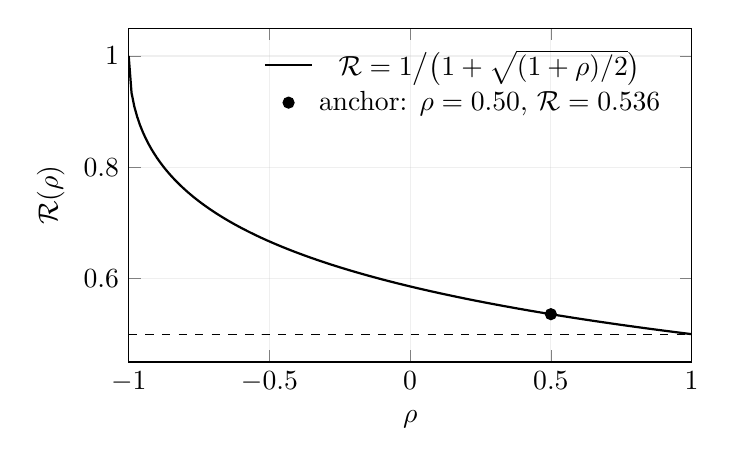
\begin{tikzpicture}
\begin{axis}[
    width=0.72\textwidth, height=0.48\textwidth,
    xlabel={$\rho$},
    ylabel={$\mathcal{R}(\rho)$},
    xmin=-1, xmax=1, ymin=0.45, ymax=1.05,
    domain=-1:1, samples=200,
    grid=both, grid style={opacity=0.25},
    legend pos=north east, legend style={draw=none, fill=none},
]
\addplot[thick] {1/(1 + sqrt((1 + x)/2))};
\addlegendentry{$\mathcal{R} = 1\big/\bigl(1 + \sqrt{(1+\rho)/2}\bigr)$}
\addplot[only marks, mark=*, mark size=2pt] coordinates {(0.5, 0.5359)};
\addlegendentry{anchor: $\rho = 0.50$, $\mathcal{R} = 0.536$}
\addplot[dashed, domain=-1:1] {0.5};
\end{axis}
\end{tikzpicture}
\caption{Equal-vol ratio $\mathcal{R}$ of the \stickycvc{} to the \stickyrho{}
$\sigma_1$-sensitivity of $\SigmaM$, as a function of $\rho$
(Corollary~\ref{cor:volII3:equalvol}). \emph{At equal vols} the ratio is
bounded in $[1/2, 1]$: there \stickycvc{} never amplifies and at most halves
the vega. With mismatched vols the band fails and \stickycvc{} can amplify
(Remark~\ref{rem:volII3:Rwarn}). The marked point is
the anchor example of Section~\ref{sec:volII3:thread}.}
\label{fig:volII3:ratio}
\end{figure}

\section{Closing the correlation thread: the anchor example}
\label{sec:volII3:thread}

%% NB (build): ratified \Cega is per correlation point ONLY; the gap-bump
%% quantity carries the chapter-local name \Cegagap (defined in Ch.2), with
%% dV/drho = 10*\Cegagap/(1-rho) the constant-\Cegagap book identity.
The volume's worked correlation example --- $\sigma_1 = \sigma_2 = \sigma =
20\%$, $\rho = 0.50$, frozen spread $\xi = \sigma\bigl(1 -
\sqrt{(1+\rho)/2}\bigr) = 0.20\,(1 - \sqrt{0.75}\,) = 0.02679$ (about $2.7$
vol points), $\Cega = +0.20$ per correlation point in the contract
normalisation ($\Cegagap = +1$ in the gap-bump quote of Chapter~2's
constant-$\Cegagap$ thread book, whose declared identity is
$\pd{V}{\rho} = 10\,\Cegagap/(1-\rho) = 20$) --- has so far run
through the basket straddle: its shadow vega ($+0.464$ per vol point), its
shadow delta ($-11.6$ dollar basis at $\volslope = -0.25$), and the
correlation update rule. The same numbers now run through the absolute
spread option, closing the loop. All figures below are re-derived from the
closed forms of this chapter; none is inherited from a numerical engine, and
in particular none relies on $\satm = \text{const}$ --- the ATM dynamics enter
explicitly through $\volslope$ where used.

\begin{example}[Anchor pricing and Greeks]\label{ex:volII3:anchor}
Take $S_1 = S_2 = 100$ (under zero rates, $F_i = S_i$ --- flagged), $T = 1$,
and the anchor vols. First the Margrabe vol: at equal vols
$\SigmaM = \sigma\sqrt{2(1 - \rho)} = 0.20\sqrt{1} = 20\%$ exactly, so
$\omM = \SigmaM\sqrt{T} = 0.20$. Then $a = b = \omM/2 = 0.10$, and:
\begin{itemize}[itemsep=0.2em]
\item \textbf{Price:} $V = 200\,\bigl(2\ncdf(0.10) - 1\bigr)
      = 200 \times 0.07966 = 15.93$. (Ballpark check:
      $0.8\,S\,\omM = 0.8 \times 100 \times 0.20 = 16$.)
\item \textbf{Symmetry constant:} $\symk = 100\,\npdf(0.10) = 39.70$, so
      $\pd{V}{\SigmaM} = 2\symk\sqrt{T} = 79.39$, i.e.\ $0.794$ per vol point
      of $\SigmaM$.
\item \textbf{Deltas:} $\pd{V}{S_1} = \pd{V}{S_2} = 2\ncdf(0.10) - 1
      = +0.0797$ on each leg.
\item \textbf{Gamma matrix:} $2\symk/\omM = 396.95$, so
      $\mathbf{\Gamma}_{11} = \mathbf{\Gamma}_{22} = +0.0397$ and
      $\mathbf{\Gamma}_{12} = -0.0397$ --- rank one, all in the spread.
\item \textbf{\stickyrho{} vegas:} each leg
      $2\symk\sqrt{T}\,\sigma(1 - \rho)/\SigmaM = 79.39 \times 0.5 = 39.70$,
      i.e.\ $0.397$ per vol point per leg; parallel $0.794$ per vol point.
\item \textbf{\stickycvc{} vegas:} each leg
      $2\symk\sqrt{T}\cdot 2\xi/\SigmaM = 79.39 \times 0.2679 = 21.27$,
      i.e.\ $0.213$ per vol point per leg; parallel
      $8\symk\xi\sqrt{T}/\SigmaM = 42.55$, i.e.\ $0.425$ per vol point.
\item \textbf{Ratio:} $\mathcal{R} = 0.213/0.397 = 0.5359
      = 1\big/(1 + \sqrt{0.75}\,)$, on the nose of
      Corollary~\ref{cor:volII3:equalvol} and
      Figure~\ref{fig:volII3:ratio}. The \stickycvc{} vega is $53.6\%$ of the
      \stickyrho{} vega at the anchor.
\end{itemize}
\end{example}

\begin{example}[Closing the shadow-Greek loop]\label{ex:volII3:shadow}
The gap between the two conventions in Example~\ref{ex:volII3:anchor} is
exactly the shadow vega of Chapter~2, computed for this payoff.
\begin{itemize}[itemsep=0.2em]
\item \textbf{Correlation exposure.} From
      $\pd{\SigmaM}{\rho} = -\sigma_1\sigma_2/\SigmaM = -0.04/0.20 = -0.20$,
      \begin{equation}\label{eq:volII3:cegaanchor}
      \pd{V}{\rho} = 2\symk\sqrt{T}\,\pd{\SigmaM}{\rho}
      = 79.39 \times (-0.20) = -15.88,
      \qquad
      \Cega = \tfrac{1}{100}\pd{V}{\rho} = -0.159
      \end{equation}
      per correlation point. Negative, as the payoff-and-risk paragraph
      promised: the absolute spread is short correlation, the anti-basket.
\item \textbf{Correlation channel.} The anchor map gives, per leg,
      $\atfixed{\pd{\rho}{\sigma_1}}{\xi}
      = (2\xi/\sigma^2)(1 - \xi/\sigma) = 1.160$, hence
      $\atfixed{\td{\rho}{\sigma}}{\xi} = 2.321$ for the parallel move ---
      the same channel slope that drove the basket book's shadow Greeks.
\item \textbf{Shadow vega.} Per the contract normalisation,
      \begin{equation}\label{eq:volII3:shvegaanchor}
      \shvega = \tfrac{1}{100}\,\pd{V}{\rho}\,
      \atfixed{\td{\rho}{\sigma}}{\xi}
      = \tfrac{1}{100} \times (-15.88) \times 2.321 = -0.368
      \end{equation}
      per vol point. Cross-check against
      Example~\ref{ex:volII3:anchor}: the parallel \stickycvc{} vega minus the
      parallel \stickyrho{} vega is $0.425 - 0.794 = -0.368$ per vol point.
      The shadow vega \emph{is} the convention gap, to the digit --- the
      additivity promised by the chain rule \eqref{eq:volII3:chain}.
\item \textbf{Shadow delta.} With the anchor's ATM slope
      $\volslope = -0.25$ (the surface dynamics of Volume~I; a $-25$
      vol-point ATM move per unit of $\lF$ --- explicitly \emph{not}
      $\satm = \text{const}$), the normaliser-ratio identity gives
      \begin{equation}\label{eq:volII3:shdeltaanchor}
      \shdelta = 100 \cdot \volslope \cdot \shvega
      = 100 \times (-0.25) \times (-0.368) = +9.2
      \end{equation}
      on the dollar basis: spot down $\Rightarrow$ ATM vols up
      $\Rightarrow$ (under \stickycvc) implied correlation up $\Rightarrow$
      $\SigmaM$ down $\Rightarrow$ the spread option loses. The position thus
      carries $+9.2$ of routed dollar delta \emph{on top of} its direct delta
      (shadow Greeks are additive per the contract's normaliser convention);
      to be flat through the routed channel the hedge must be \emph{short} a
      further $9.2$ of dollar delta.
\end{itemize}
The thread is now closed. The basket straddle of Chapter~2 carried
$\shvega = +0.464$ and $\shdelta = -11.6$; the absolute spread at the same
anchor carries $\shvega = -0.368$ and $\shdelta = +9.2$. The basket figures
pass the same arithmetic as \eqref{eq:volII3:shvegaanchor}: with the basket's
$\pd{V}{\rho} = +20$ (Cega $+0.20$ per correlation point, $+1$ gap-bump),
$\tfrac{1}{100} \times 20 \times 2.321 = +0.464$ and $100 \times (-0.25)
\times 0.464 = -11.6$, consistent to the digit. Same surface, same
correlation channel $\atfixed{\td{\rho}{\sigma}}{\xi} = 2.321$, opposite
signs --- because $\pd{\sB}{\rho} > 0$ while $\pd{\SigmaM}{\rho} < 0$. A desk
running the dispersion pair (long the spread option, short the basket
straddle, or vice versa) nets the two shadow-Greek columns; a desk marking one
leg \stickyrho{} and the other \stickycvc{} books a phantom vega of order
half its true exposure. That inconsistency, not the model, is the free-money
leak to guard against.
\end{example}

\begin{figure}[ht]
\centering
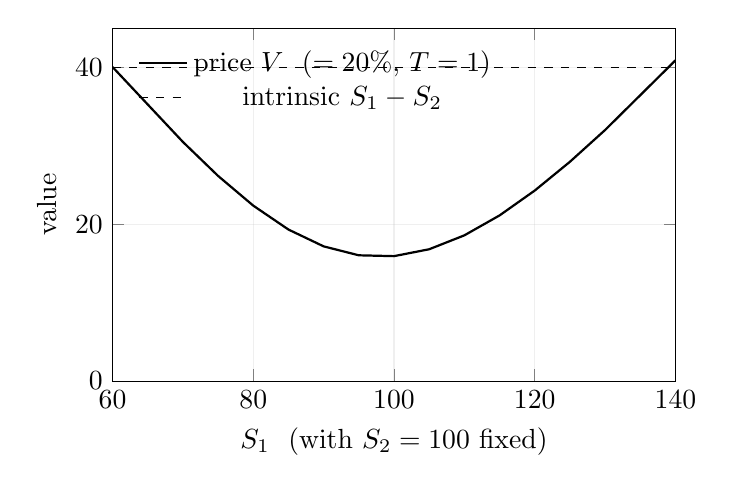
\begin{tikzpicture}
\begin{axis}[
    width=0.72\textwidth, height=0.5\textwidth,
    xlabel={$S_1$ \ (with $S_2 = 100$ fixed)},
    ylabel={value},
    xmin=60, xmax=140, ymin=0, ymax=45,
    grid=both, grid style={opacity=0.25},
    legend pos=north west, legend style={draw=none, fill=none},
]
\addplot[thick] coordinates {
(60, 40.052) (70, 30.496) (75, 26.162) (80, 22.372) (85, 19.323)
(90, 17.178) (95, 16.039) (100, 15.931) (105, 16.811) (110, 18.584)
(115, 21.124) (120, 24.295) (125, 27.965) (130, 32.018) (140, 40.900)
};
\addlegendentry{price $V$ \ ($\SigmaM = 20\%$, $T = 1$)}
\addplot[dashed, domain=60:140, samples=2] {abs(x - 100)};
\addlegendentry{intrinsic $\abs{S_1 - S_2}$}
\end{axis}
\end{tikzpicture}
\caption{The absolute spread at the anchor ($\SigmaM = 20\%$, $T = 1$,
$S_2 = 100$): a straddle on the spread. The minimum-value point sits at
$S_1 = S_2$, where the deltas \eqref{eq:volII3:deltas} are both small and
positive and the rank-one gamma \eqref{eq:volII3:gamma} peaks; as $T \to 0$
the price collapses onto the intrinsic kink and the position pins.}
\label{fig:volII3:payoff}
\end{figure}

\section{How the results cohere}
\label{sec:volII3:cohere}

\begin{enumerate}[label=(\arabic*)]
\item \textbf{Symmetric pricing.} The payoff $\abs{S_1 - S_2}$ is the sum of
the two exchange options, and its price admits the symmetric representation
\eqref{eq:volII3:price}. The spot deltas \eqref{eq:volII3:deltas} and the
rank-one gamma matrix \eqref{eq:volII3:gamma} follow in closed form from that
symmetry, with the constant $\symk = S_1\npdf(a) = S_2\npdf(b)$ carrying all
the second-order structure.

\item \textbf{Two re-marking conventions.} Under \stickyrho{} the relevant
sensitivity is the direct partial \eqref{eq:volII3:dSMrho}; under \stickycvc{}
the exact correlation map \eqref{eq:volII3:rhomap} collapses the Margrabe
variance to \eqref{eq:volII3:SM2xi} and the routed derivative is
\eqref{eq:volII3:dSMxi}. Multiplying either by $\pd{V}{\SigmaM} =
2\symk\sqrt{T}$ gives the corresponding vegas, \eqref{eq:volII3:vegarho} and
\eqref{eq:volII3:vegaxi}.

\item \textbf{The comparison is exact.}
Proposition~\ref{prop:volII3:chain} isolates the \stickycvc{} correction as
the routed chain-rule term
$\pd{\SigmaM}{\rho}\,\atfixed{\pd{\rho}{\sigma_1}}{\xi}$, negative on the
admissibility domain $\xi \le \min(\sigma_1, \sigma_2)$ of
Corollary~\ref{cor:volII3:cvcadmiss}; Proposition~\ref{prop:volII3:ratio}
gives the exact ratio (where the \stickyrho{} sensitivity is non-zero,
$\sigma_1 \ne \rho\sigma_2$), which at equal vols is
$\mathcal{R} = 1\big/\bigl(1 + \sqrt{(1+\rho)/2}\bigr) \in [1/2, 1]$. \emph{At
equal vols} the \stickycvc{} vega is never larger than the \stickyrho{} vega,
and near $\rho \approx 1$ it is almost exactly half. With mismatched vols only
the signed inequality \eqref{eq:volII3:signineq} survives; in magnitude
\stickycvc{} can amplify, as Remark~\ref{rem:volII3:Rwarn}'s $\mathcal{R} =
1.89$ counterexample shows.

\item \textbf{The correlation thread closes.} At the volume's anchor
($\sigma = 20\%$, $\rho = 0.50$, $\xi = 0.02679$) the spread option's shadow
vega, $-0.368$ per vol point, equals the gap between its \stickycvc{} and
\stickyrho{} parallel vegas to the digit, and its shadow delta is $+9.2$ at
$\volslope = -0.25$ --- equal channel, opposite sign to the basket book. The
shadow Greeks are exactly the difference between the two conventions, they
vanish under \stickyrho{}, and they net across a dispersion pair. What must
never happen is a book marked half in one convention and half in the other.
\end{enumerate}
%% ============================================================================
%% frag_volII_ch4.tex -- Vol II Ch 4: Correlation-Matrix Admissibility (n-name)
%% Author: NAZAROV. Governed by NOTATION_CONTRACT.md; macros from build/preamble.tex.
%% Closes the admissibility ladder: single-name wing & convexity (Vol I Ch 2)
%% -> two-name xi >= 0, rho <= 1 (Vol II Ch 1) -> n-name PSD / Schur (here).
%% No F = S collapse is used anywhere in this chapter (no forward appears in a
%% derivation); constraint C1 is cited where the per-name vols enter.
%% ============================================================================

\chapter{Correlation Admissibility for $n$ Names: Schur Complements and Blockwise Modification}
\label{ch:admiss}

\section{The admissibility ladder}\label{sec:admiss:ladder}

Every rung of this corpus's no-arbitrage theory has the same shape: a quoted
object is admissible if and only if it lies in a convex feasible set, and the
interesting economics happens at the boundary of that set.

\begin{itemize}
  \item \textbf{Rung 1 (one name).} Volume~I, Chapter~2: a single-name surface
        $\sigma(\mln,\lF,T) = \satm(\lF,T) + \ssm(\mln,T)$ is admissible only
        if the call prices $C(K,T)$ it induces are convex in $K$ (no butterfly
        arbitrage --- equivalently, the risk-neutral density is nonnegative),
        the wings of $\ssm(\mln,T)$ grow slowly enough in $\abs{\mln}$
        that the density integrates, and the total variance $\sigma^2 T$ is
        non-decreasing in $T$ (no calendar-spread arbitrage) --- conditions
        (A2), the Lee wing control, and (A3) of the admissible set of that
        chapter. The feasible set is a convex set of
        smile functions; its boundary is a zero of the density.
  \item \textbf{Rung 2 (two names).} Chapter~1 of the present volume: the
        basket volatility $\sB$, the mean volatility $\sbmean =
        \tfrac{1}{2}(\sigma_1+\sigma_2)$, and the implied correlation $\rho$
        are tied by $\sB^2 = \tfrac14\sigma_1^2 + \tfrac14\sigma_2^2 +
        \tfrac12\rho\sigma_1\sigma_2$, and the pair
        $(\sigma_1,\sigma_2,\rho)$ is admissible if and only if
        $\rho \in [-1,1]$ --- equivalently, if and only if the $2\times 2$
        matrix $\bigl(\begin{smallmatrix} 1 & \rho \\ \rho & 1
        \end{smallmatrix}\bigr)$ is positive semidefinite. The upper endpoint
        is the vanishing of the basket vol spread: $\xi = \sbmean - \sB \ge 0$
        with equality exactly at $\rho = 1$. The feasible set is an interval;
        its boundary is a singular $2\times 2$ correlation matrix.
  \item \textbf{Rung 3 ($n$ names).} This chapter. With $n$ names the quoted
        object is the full matrix $\Omega$ of pairwise implied correlations,
        and admissibility is positive semidefiniteness of $\Omega$. The
        feasible set is a compact convex body (the set of correlation
        matrices); its boundary is the locus of singular $\Omega$. The tool
        that makes this rung computable --- that reduces ``is the whole
        matrix admissible?'' to conditions on the piece being changed --- is
        the Schur complement.
\end{itemize}

Throughout, the per-name volatilities that accompany $\Omega$ are the
single-name ATM volatilities of the mandated decomposition,
$\sigma_i \equiv \satmi{i}(\lFi{i}, T)$ evaluated at each name's current
forward (constraint C1). No forward appears in any derivation of this
chapter, so no zero-rate collapse is invoked anywhere in it: correlation
admissibility is a statement of pure linear algebra and Gaussian
conditioning, sitting on top of --- and independent of --- the surface
dynamics of the earlier rungs.

\begin{figure}[ht]
\centering
\begin{tikzpicture}[
  rung/.style={draw, rounded corners=2pt, align=left, inner sep=7pt,
               text width=0.72\textwidth, font=\small}]
  \node[rung] (r1) at (0,0)
    {\textbf{Rung 1 --- one name (Vol.\ I, Ch.\ 2).}
     Convexity of $C(K,T)$ in $K$, wing growth of $\ssm(\mln,T)$, and
     calendar monotonicity of total variance: the risk-neutral density is
     nonnegative at every expiry.};
  \node[rung] (r2) at (0,2.1)
    {\textbf{Rung 2 --- two names (Ch.\ 1).}
     $\xi = \sbmean - \sB \ge 0 \iff \rho \le 1$; admissibility is
     $\bigl(\begin{smallmatrix} 1 & \rho \\ \rho & 1\end{smallmatrix}\bigr)
     \succeq 0$, i.e.\ $\abs{\rho} \le 1$.};
  \node[rung] (r3) at (0,4.2)
    {\textbf{Rung 3 --- $n$ names (this chapter).}
     $\Omega \succeq 0$, certified blockwise:
     $\Omega \succeq 0 \iff \SchurC{B}{\Omega} \succeq 0$ given $B \succ 0$.};
  \draw[->, thick] (r1.north) -- (r2.south)
    node[midway, right=2pt, font=\footnotesize] {add a name};
  \draw[->, thick] (r2.north) -- (r3.south)
    node[midway, right=2pt, font=\footnotesize] {condition on the rest};
\end{tikzpicture}
\caption{The admissibility ladder. Each rung is the boundary of a convex
feasible set; rung 2 is recovered from rung 3 by taking an empty
conditioning block (Remark~\ref{rem:admiss:rung2}).}
\label{fig:admiss:ladder}
\end{figure}

\subsection{Local notation}\label{sec:admiss:notation}

%% FORMALIS: requesting a one-line contract annotation on the Schur_B(M) row,
%% recording that the block letter C in its own gloss (A - C^T B^{-1} C)
%% collides with the ratified call price C(K,T) (owner I.1), and that this
%% chapter resolves the collision by the declaration below (bare C =
%% cross-block; call price always written with its arguments).
The following symbols are scoped to this chapter. Block letters $A$, $B$,
$C$ are those of the ratified Schur entry
$\SchurC{B}{M} = A - C^{\mathsf T} B^{-1} C$; one of them collides with the
ratified table, and the collision is resolved by declaration rather than
denied. The glyph $C$ is owned in the ratified table by the European call
price $C(K,T)$ (owner I.1). In this chapter, \emph{bare} $C$ always denotes
the cross-block of the partition \eqref{eq:admiss:block} --- the contract's
own gloss for $\SchurC{B}{M}$ already uses the block letter --- while the
call price is always written with its arguments, $C(K,T)$, and appears only
in the rung-1 ladder prose of Sections~\ref{sec:admiss:ladder}
and~\ref{sec:admiss:closing}, never in a derivation of this chapter. No
other local symbol collides with the ratified table. Index sets are
calligraphic, $\mathcal{I}$ and $\mathcal{J}$, with sizes
$n_{\mathcal I} = \abs{\mathcal I}$ and $n_{\mathcal J} = \abs{\mathcal J}$
(the glyphs $\mathcal J$ and $n_{\mathcal J}$ are distinct from the
observation count $J$ of the calibration chapters). $\mathrm{Id}_p$ is the
$p \times p$ identity, $\mathbf{1}$ the all-ones column vector,
$\mathbf{1}\mathbf{1}^{\mathsf T}$ the all-ones matrix. $\Theta :=
\Omega^{-1}$ is the precision matrix. $\Pi := C^{\mathsf T} B^{-1} C$ is the
explained block, $\Sigma_{\mathcal I | \mathcal J}$ the conditional
covariance, $R$ the conditional correlation matrix, $D$ the diagonal matrix
of conditional variances, $G := C^{\mathsf T} B^{-1}$ the regression matrix,
$\lambda \in [0,1]$ the blending weight, and $\mu_{\min}(\cdot)$,
$\mu_{\max}(\cdot)$ the extreme eigenvalues of a symmetric matrix. For the
single-entry bound: $q_u := u^{\mathsf T} B^{-1} u$,
$q_v := v^{\mathsf T} B^{-1} v$, centre $\bar\rho_{ij} :=
u^{\mathsf T} B^{-1} v$, half-width $\eta_{ij} :=
\sqrt{(1-q_u)(1-q_v)}$, and $t \in [-1,1]$ the partial-correlation
coordinate. Inner products are written $x^{\mathsf T} y$ throughout; the
bra-ket calculus is reserved for the calibration block of Volume~I and does
not appear in this chapter. Two near-misses are declared,
though neither is a contract collision: the conditional
covariance is written $\Sigma_{\mathcal I|\mathcal J}$ (bare $\Sigma$
appears only as the local abbreviation $\Sigma := \SchurC{B}{M}$ inside the
statements and proofs of Section~\ref{sec:admiss:schur}) and is unrelated
to the Margrabe volatility $\SigmaM$ of Chapter~3; the extreme eigenvalues
$\mu_{\min}(\cdot)$, $\mu_{\max}(\cdot)$ are unrelated to the kernel
centres $\mu_i$ of Volume~I.

\begin{definition}[Admissible correlation matrix]\label{def:admiss:corr}
A matrix $\Omega \in \mathbb{R}^{n \times n}$ is an \emph{admissible
correlation matrix} if it is symmetric, has unit diagonal
($\Omega_{ii} = 1$ for all $i$), and is positive semidefinite,
$\Omega \succeq 0$; $\Omega \succ 0$ denotes the positive-definite case.
The set of admissible $n \times n$ correlation matrices is denoted
$\mathcal{E}_n$ and called the \emph{elliptope}; it is compact and convex.
Convexity and closedness hold because $\mathcal{E}_n$ is an intersection of
the PSD cone (closed, convex) with the affine constraints $\Omega_{ii} = 1$;
boundedness needs one more line: PSD-ness of every $2 \times 2$ principal
minor together with the unit diagonal forces
$1 - \Omega_{ij}^2 \ge 0$, i.e.\ $\abs{\Omega_{ij}} \le 1$ for all $i, j$,
so $\mathcal{E}_n$ is bounded, and closed plus bounded in
$\mathbb{R}^{n \times n}$ is compact.
\end{definition}

Admissibility is not decoration. If $\Omega \not\succeq 0$ there is a vector
$x$ with $x^{\mathsf T} \Omega x < 0$: the portfolio with weights
proportional to $x$ (in vol-normalised units) has \emph{negative variance}.
Every Monte Carlo engine, every basket vol, every Margrabe volatility
$\SigmaM$ built on such a matrix is pricing an object that cannot exist.

\section{The Schur complement and the positivity criterion}
\label{sec:admiss:schur}

\begin{definition}[Schur complement]\label{def:admiss:schurcomp}
Let $M \in \mathbb{R}^{n \times n}$ be symmetric, partitioned as
\begin{equation}\label{eq:admiss:block}
  M \;=\; \begin{pmatrix} A & C^{\mathsf T} \\ C & B \end{pmatrix},
  \qquad
  A \in \mathbb{R}^{n_{\mathcal I} \times n_{\mathcal I}},\quad
  B \in \mathbb{R}^{n_{\mathcal J} \times n_{\mathcal J}},\quad
  C \in \mathbb{R}^{n_{\mathcal J} \times n_{\mathcal I}},
\end{equation}
with $n_{\mathcal I} + n_{\mathcal J} = n$. If $B \succ 0$, the
\emph{Schur complement of $B$ in $M$} is
\begin{equation}\label{eq:admiss:schurdef}
  \SchurC{B}{M} \;:=\; A - C^{\mathsf T} B^{-1} C .
\end{equation}
\end{definition}

The entire chapter rests on one algebraic identity: the block partition
\eqref{eq:admiss:block} can be \emph{diagonalised by congruence}, with the
Schur complement appearing as the residual block.

\begin{lemma}[Block congruence]\label{lem:admiss:congruence}
Let $M$ be as in \eqref{eq:admiss:block} with $B \succ 0$, and set
$\Sigma := \SchurC{B}{M}$. Then
\begin{equation}\label{eq:admiss:ldl}
  M \;=\; L^{\mathsf T}
  \begin{pmatrix} \Sigma & 0 \\ 0 & B \end{pmatrix}
  L,
  \qquad
  L \;=\; \begin{pmatrix} \mathrm{Id}_{n_{\mathcal I}} & 0 \\
                          B^{-1} C & \mathrm{Id}_{n_{\mathcal J}}
          \end{pmatrix},
\end{equation}
and $L$ is invertible.
\end{lemma}

\begin{proof}
Multiply out the right-hand side:
\[
  L^{\mathsf T} \begin{pmatrix} \Sigma & 0 \\ 0 & B \end{pmatrix} L
  = \begin{pmatrix} \mathrm{Id} & C^{\mathsf T} B^{-1} \\ 0 & \mathrm{Id} \end{pmatrix}
    \begin{pmatrix} \Sigma & 0 \\ 0 & B \end{pmatrix}
    \begin{pmatrix} \mathrm{Id} & 0 \\ B^{-1} C & \mathrm{Id} \end{pmatrix}
  = \begin{pmatrix} \Sigma + C^{\mathsf T} B^{-1} C & C^{\mathsf T} \\
                    C & B \end{pmatrix}
  = M,
\]
using $C^{\mathsf T} B^{-1} B = C^{\mathsf T}$ and
$\Sigma + C^{\mathsf T} B^{-1} C = A$. The matrix $L$ is block
lower-triangular with identity diagonal blocks, hence has determinant $1$
and is invertible.
\end{proof}

\begin{theorem}[Schur positivity criterion]\label{thm:admiss:criterion}
Let $M$ be as in \eqref{eq:admiss:block} with $B \succ 0$. Then
\[
  M \succeq 0
  \quad\Longleftrightarrow\quad
  \SchurC{B}{M} \succeq 0,
\]
and likewise $M \succ 0 \iff \SchurC{B}{M} \succ 0$.
\end{theorem}

\begin{proof}
By Lemma~\ref{lem:admiss:congruence}, for any $x \in \mathbb{R}^n$, writing
$y = L x$,
\[
  x^{\mathsf T} M x
  = y^{\mathsf T} \begin{pmatrix} \Sigma & 0 \\ 0 & B \end{pmatrix} y
  = y_{\mathcal I}^{\mathsf T} \Sigma\, y_{\mathcal I}
    + y_{\mathcal J}^{\mathsf T} B\, y_{\mathcal J}.
\]
Since $L$ is invertible, $x \mapsto y$ is a bijection of $\mathbb{R}^n$.
If $\Sigma \succeq 0$, both terms on the right are nonnegative
($B \succ 0$ by hypothesis), so $M \succeq 0$. Conversely, if
$\Sigma \not\succeq 0$, pick $z$ with $z^{\mathsf T} \Sigma z < 0$ and take
$y = (z, 0)$: the corresponding $x = L^{-1} y$ gives
$x^{\mathsf T} M x = z^{\mathsf T} \Sigma z < 0$, so $M \not\succeq 0$.
The positive-definite statement is identical with strict inequalities,
noting that $y \ne 0 \iff x \ne 0$.
\end{proof}

\subsection{The Schur complement is a conditional covariance}
\label{sec:admiss:conditional}

The criterion of Theorem~\ref{thm:admiss:criterion} is pure linear algebra,
but its content is probabilistic, and the probabilistic reading is what
makes every construction in this chapter interpretable. It is the same
Gaussian-conditioning identity that drives the Bayesian update of the
calibration filter in Volume~I, Chapter~4: there, the posterior covariance
of the parameter ket given an observation is the Schur complement of the
observation block in the joint covariance; here, the roles are played by
two blocks of names.

\begin{proposition}[Conditional covariance identity]\label{prop:admiss:condcov}
Let $(X_{\mathcal I}, X_{\mathcal J})$ be a zero-mean jointly Gaussian
vector with covariance matrix $M$ partitioned as in
\eqref{eq:admiss:block}, $B \succ 0$. Then
\begin{equation}\label{eq:admiss:condcov}
  \Cov\bigl(X_{\mathcal I} \mid X_{\mathcal J}\bigr)
  \;=\; \SchurC{B}{M} \;=\; A - C^{\mathsf T} B^{-1} C,
\end{equation}
and the conditional mean is
$\E[X_{\mathcal I} \mid X_{\mathcal J}] = G X_{\mathcal J}$ with
$G = C^{\mathsf T} B^{-1}$.
\end{proposition}

\begin{proof}[Proof (regression / best linear predictor)]
Because the vector is jointly Gaussian, the conditional expectation is
linear: $\E[X_{\mathcal I} \mid X_{\mathcal J}] = G X_{\mathcal J}$ for some
$G \in \mathbb{R}^{n_{\mathcal I} \times n_{\mathcal J}}$, and the
conditional covariance is the covariance of the residual
$X_{\mathcal I} - G X_{\mathcal J}$. The matrix $G$ is pinned down by the
orthogonality of the residual to the conditioning variables:
\[
  0 = \Cov\bigl(X_{\mathcal I} - G X_{\mathcal J},\, X_{\mathcal J}\bigr)
    = \Cov(X_{\mathcal I}, X_{\mathcal J}) - G \Cov(X_{\mathcal J}, X_{\mathcal J})
    = C^{\mathsf T} - G B,
\]
so $G = C^{\mathsf T} B^{-1}$. The residual covariance is then
\begin{align*}
  \Cov\bigl(X_{\mathcal I} - G X_{\mathcal J}\bigr)
  &= A - G C - C^{\mathsf T} G^{\mathsf T} + G B G^{\mathsf T} \\
  &= A - C^{\mathsf T} B^{-1} C - C^{\mathsf T} B^{-1} C
       + C^{\mathsf T} B^{-1} B B^{-1} C
   \;=\; A - C^{\mathsf T} B^{-1} C,
\end{align*}
the middle two terms cancelling against the last. For a Gaussian vector the
residual is independent of $X_{\mathcal J}$, so its covariance is exactly
the conditional covariance.
\end{proof}

A second, purely algebraic route to the same identity runs through the
precision matrix; it is recorded because the precision-matrix block is
needed for the partial-correlation coordinate of
Section~\ref{sec:admiss:single}.

\begin{proposition}[Block inverse]\label{prop:admiss:blockinv}
Let $M \succ 0$ be partitioned as in \eqref{eq:admiss:block} and set
$\Sigma := \SchurC{B}{M}$. Then the $\mathcal I \times \mathcal I$ block of
$M^{-1}$ is $\Sigma^{-1}$:
\[
  M^{-1} \;=\; \begin{pmatrix} \Sigma^{-1} & * \\ * & * \end{pmatrix}.
\]
\end{proposition}

\begin{proof}
Write $M^{-1} = \bigl(\begin{smallmatrix} X & Y^{\mathsf T} \\ Y & Z
\end{smallmatrix}\bigr)$ with $X \in \mathbb{R}^{n_{\mathcal I} \times
n_{\mathcal I}}$. The identity $M M^{-1} = \mathrm{Id}_n$ gives, in its
first block column,
\[
  A X + C^{\mathsf T} Y = \mathrm{Id}_{n_{\mathcal I}},
  \qquad
  C X + B Y = 0 .
\]
From the second equation $Y = -B^{-1} C X$; substituting into the first,
$\bigl(A - C^{\mathsf T} B^{-1} C\bigr) X = \mathrm{Id}_{n_{\mathcal I}}$,
i.e.\ $\Sigma X = \mathrm{Id}$, so $X = \Sigma^{-1}$.
\end{proof}

Combining Proposition~\ref{prop:admiss:blockinv} with the standard Gaussian
conditioning formula
$\Cov(X_{\mathcal I} \mid X_{\mathcal J}) = \bigl([M^{-1}]_{\mathcal I
\mathcal I}\bigr)^{-1}$ recovers \eqref{eq:admiss:condcov} a second time:
the conditional covariance is the inverse of the
$\mathcal I \times \mathcal I$ precision block, which is
$(\Sigma^{-1})^{-1} = \Sigma$.

\begin{remark}[Explained plus residual]\label{rem:admiss:explained}
Proposition~\ref{prop:admiss:condcov} splits the block $A$ of the generic
matrix $M$ of \eqref{eq:admiss:block} into two PSD pieces,
\begin{equation}\label{eq:admiss:split}
  A \;=\; \Pi + \Sigma_{\mathcal I | \mathcal J},
  \qquad
  \Pi := C^{\mathsf T} B^{-1} C
       = \Cov\bigl(\E[X_{\mathcal I} \mid X_{\mathcal J}]\bigr),
  \qquad
  \Sigma_{\mathcal I | \mathcal J} := \SchurC{B}{M}
       = \Cov\bigl(X_{\mathcal I} \mid X_{\mathcal J}\bigr):
\end{equation}
the covariance inside $\mathcal I$ that is \emph{explained} through
$\mathcal J$, plus the covariance of what remains after the best linear
prediction. Both pieces are PSD: for any $x$,
$x^{\mathsf T} \Pi x = (C x)^{\mathsf T} B^{-1} (C x) \ge 0$ since
$B \succ 0$, and $\Sigma_{\mathcal I|\mathcal J} \succeq 0$ by
Theorem~\ref{thm:admiss:criterion} whenever $M \succeq 0$. The
$\Omega$-specialised version of \eqref{eq:admiss:split} appears as
\eqref{eq:admiss:APi} below. This is the analysis-of-variance decomposition of
multivariate regression, and it is the load-bearing structure of
Sections~\ref{sec:admiss:block}--\ref{sec:admiss:blend}: once $B$ and $C$
are frozen, $\Pi$ is frozen, and \emph{all} remaining freedom lives in the
residual term.
\end{remark}

\section{One entry at a time: the Schur bound}\label{sec:admiss:single}

The smallest possible modification changes a single
correlation entry and keeps everything else. This is precisely the bump that
defines $\Cega$ hedging in Chapters~1--2 --- a one-correlation-point move of
one pair --- and the theorem below says exactly how far such a bump may go
before the model leaves the elliptope.

Let $\Omega \in \mathcal{E}_n$ and fix two distinct indices $i, j$. Reorder
the names so that $i$ and $j$ come first, and let
$\mathcal{R} = \{1, \dots, n\} \setminus \{i, j\}$ be the conditioning set.
In this ordering,
\begin{equation}\label{eq:admiss:threeblock}
  \Omega \;=\;
  \begin{pmatrix}
    1 & \rho & u^{\mathsf T} \\
    \rho & 1 & v^{\mathsf T} \\
    u & v & B
  \end{pmatrix},
  \qquad
  u = \Omega_{\mathcal{R} i}, \quad
  v = \Omega_{\mathcal{R} j}, \quad
  B = \Omega_{\mathcal{R} \mathcal{R}},
\end{equation}
where $\rho := \Omega_{ij}$ is the entry allowed to move, and $u$, $v$,
$B$ are held fixed.

\begin{assumption}[Nondegenerate conditioning block]\label{ass:admiss:B}
Throughout Sections~\ref{sec:admiss:single}--\ref{sec:admiss:blend}, the
fixed block $B$ is positive definite, $B \succ 0$. (If $B$ is merely PSD
and singular, some name in the conditioning set is a deterministic linear
combination of the others; remove the redundant names first.)
\end{assumption}

Define the scalars
\begin{equation}\label{eq:admiss:scalars}
  q_u := u^{\mathsf T} B^{-1} u,
  \qquad
  q_v := v^{\mathsf T} B^{-1} v,
  \qquad
  \bar\rho_{ij} := u^{\mathsf T} B^{-1} v,
  \qquad
  \eta_{ij} := \sqrt{(1 - q_u)(1 - q_v)} .
\end{equation}

\begin{theorem}[Schur bound for a single entry]\label{thm:admiss:single}
Let $\Omega$ be as in \eqref{eq:admiss:threeblock} with $B \succ 0$, and
suppose $q_u \le 1$ and $q_v \le 1$ (automatic when the unmodified matrix is
admissible). Then the matrix $\Omega$ with entry $\Omega_{ij} = \rho$ is an
admissible correlation matrix if and only if
\begin{equation}\label{eq:admiss:interval}
  \bar\rho_{ij} - \eta_{ij}
  \;\le\; \rho \;\le\;
  \bar\rho_{ij} + \eta_{ij} .
\end{equation}
\end{theorem}

\begin{proof}
First, the parenthetical in the hypothesis. If the unmodified matrix is
admissible, its principal submatrix on the index set $\{i\} \cup \mathcal{R}$
is PSD; applying Theorem~\ref{thm:admiss:criterion} to that submatrix with
conditioning block $B \succ 0$ shows that its Schur complement, the scalar
$1 - u^{\mathsf T} B^{-1} u = 1 - q_u$, is nonnegative, i.e.\ $q_u \le 1$;
likewise $q_v \le 1$ from the submatrix on $\{j\} \cup \mathcal{R}$.

For the main statement, apply Theorem~\ref{thm:admiss:criterion} with
$\mathcal I = \{i, j\}$ and $\mathcal J = \mathcal{R}$. The Schur complement
of $B$ is the $2 \times 2$ matrix
\[
  \Sigma_{ij|\mathcal{R}}
  = \begin{pmatrix} 1 & \rho \\ \rho & 1 \end{pmatrix}
    - \begin{pmatrix} u^{\mathsf T} \\ v^{\mathsf T} \end{pmatrix}
      B^{-1} \begin{pmatrix} u & v \end{pmatrix}
  = \begin{pmatrix}
      1 - q_u & \rho - \bar\rho_{ij} \\
      \rho - \bar\rho_{ij} & 1 - q_v
    \end{pmatrix}.
\]
A symmetric $2 \times 2$ matrix is PSD if and only if both diagonal entries
and the determinant are nonnegative. The diagonal conditions are the
hypotheses $q_u \le 1$, $q_v \le 1$; the determinant condition is
\[
  (1 - q_u)(1 - q_v) - (\rho - \bar\rho_{ij})^2 \;\ge\; 0
  \quad\Longleftrightarrow\quad
  \abs{\rho - \bar\rho_{ij}} \;\le\; \eta_{ij},
\]
which is \eqref{eq:admiss:interval}. Unit diagonal and symmetry are
untouched by the modification.
\end{proof}

\begin{corollary}[Partial-correlation coordinate]\label{cor:admiss:partial}
Assume additionally $q_u < 1$, $q_v < 1$. Then every admissible value of
the entry can be written
\begin{equation}\label{eq:admiss:param}
  \rho \;=\; \bar\rho_{ij} + \eta_{ij}\, t,
  \qquad t \in [-1, 1] .
\end{equation}
On the \emph{open} interval $t \in (-1, 1)$ the matrix is positive
definite --- $\Sigma_{ij|\mathcal{R}}$ has positive diagonal ($q_u, q_v <
1$) and determinant $\eta_{ij}^2 (1 - t^2) > 0$, hence
$\Sigma_{ij|\mathcal{R}} \succ 0$ and $\Omega \succ 0$ by
Theorem~\ref{thm:admiss:criterion} --- so $\Theta := \Omega^{-1}$ exists
and the coordinate is the partial correlation:
\begin{equation}\label{eq:admiss:paramid}
  t \;=\; \rho_{ij \cdot \mathcal{R}}
  \;:=\; -\frac{\Theta_{ij}}{\sqrt{\Theta_{ii}\Theta_{jj}}}
  \;=\; \frac{\rho - \bar\rho_{ij}}{\eta_{ij}},
  \qquad t \in (-1, 1) .
\end{equation}
The endpoints $t = \pm 1$ are exactly the singular boundary of the
elliptope: there $\Sigma_{ij|\mathcal{R}}$, and hence $\Omega$, drops rank,
$\Theta$ is undefined, and the identity \eqref{eq:admiss:paramid} holds
only in the limit $t \to \pm 1$ (both sides being continuous in $\rho$ on
the open interval).
\end{corollary}

\begin{proof}
The parametrisation \eqref{eq:admiss:param} over the closed interval is a
restatement of Theorem~\ref{thm:admiss:single}. Now fix $\abs{t} < 1$, so
that $\Omega \succ 0$ as computed in the statement and $\Theta$ exists.
By Proposition~\ref{prop:admiss:blockinv} (with $i, j$ ordered first), the
top-left $2 \times 2$ block of $\Theta$ is $\Sigma_{ij|\mathcal{R}}^{-1}$.
Inverting the $2 \times 2$ matrix from the previous proof,
\[
  \Sigma_{ij|\mathcal{R}}^{-1}
  = \frac{1}{\det \Sigma_{ij|\mathcal{R}}}
    \begin{pmatrix}
      1 - q_v & -(\rho - \bar\rho_{ij}) \\
      -(\rho - \bar\rho_{ij}) & 1 - q_u
    \end{pmatrix},
\]
so
\[
  -\frac{\Theta_{ij}}{\sqrt{\Theta_{ii}\Theta_{jj}}}
  = \frac{\rho - \bar\rho_{ij}}
         {\sqrt{(1 - q_u)(1 - q_v)}}
  = \frac{\rho - \bar\rho_{ij}}{\eta_{ij}} ,
\]
the determinant prefactors cancelling in the ratio. Theorem
\ref{thm:admiss:single} says admissibility is $\abs{t} \le 1$, with
equality forcing $\det \Sigma_{ij|\mathcal{R}} = 0$.
\end{proof}

The reading of \eqref{eq:admiss:param} is the Bayesian one: $\bar\rho_{ij}$
is the correlation between $i$ and $j$ \emph{already implied by their common
exposure to the rest of the market} (the explained part, through
$\Pi$), and $\eta_{ij}$ is the room left over --- the geometric mean of the
two conditional standard deviations. The market may quote any residual
(partial) correlation $t$ in $[-1, 1]$ on top of the explained centre; it
may not quote more than perfect conditional correlation.

\begin{remark}[Rung 2 recovered]\label{rem:admiss:rung2}
For $n = 2$ the conditioning set $\mathcal{R}$ is empty: $q_u = q_v = 0$,
$\bar\rho_{ij} = 0$, $\eta_{ij} = 1$, and \eqref{eq:admiss:interval}
collapses to $-1 \le \rho \le 1$ --- the two-name admissibility interval of
Chapter~1, whose upper endpoint is $\xi = 0$. The ladder is consistent:
rung 2 is rung 3 with nothing to condition on.
\end{remark}

\begin{example}[A three-name Schur bound, worked in full]
\label{ex:admiss:threename}
Take $n = 3$ and let name $3$ be the conditioning set for the pair
$(1, 2)$, with
\[
  \Omega_{13} = 0.6, \qquad \Omega_{23} = 0.5, \qquad B = (1),
\]
so $u = (0.6)$, $v = (0.5)$. The scalars \eqref{eq:admiss:scalars} are
\[
  q_u = 0.36, \qquad q_v = 0.25, \qquad
  \bar\rho_{12} = 0.6 \times 0.5 = 0.30, \qquad
  \eta_{12} = \sqrt{0.64 \times 0.75} = \sqrt{0.48} \approx 0.6928 .
\]
Theorem~\ref{thm:admiss:single} gives the feasible interval
\[
  \rho_{12} \;\in\; [\,0.30 - 0.6928,\; 0.30 + 0.6928\,]
            \;=\; [-0.3928,\; 0.9928] .
\]
Cross-check against the determinant of the full $3 \times 3$ matrix,
$\det \Omega = 1 + 2 \rho_{12} \Omega_{13} \Omega_{23} - \rho_{12}^2 -
\Omega_{13}^2 - \Omega_{23}^2 = -\rho_{12}^2 + 0.6\, \rho_{12} + 0.39$: its
roots are $\rho_{12} = \bigl(0.6 \pm \sqrt{0.36 + 1.56}\bigr)/2 =
(0.6 \pm 1.3856)/2$, i.e.\ $-0.3928$ and $0.9928$ --- the interval
endpoints, as they must be. A quoted $\rho_{12} = 0.80$ is admissible, with
partial-correlation coordinate $t = (0.80 - 0.30)/0.6928 \approx 0.72$; a
quoted $\rho_{12} = -0.50$ is \emph{not} admissible: no joint distribution
of the three names exists with these pairwise correlations, however
plausible each pair looks in isolation. The interval is asymmetric: the
common exposure to name $3$ shifts it upward, squeezing out
anticorrelation while leaving near-perfect positive correlation available.
\end{example}

\begin{figure}[ht]
\centering
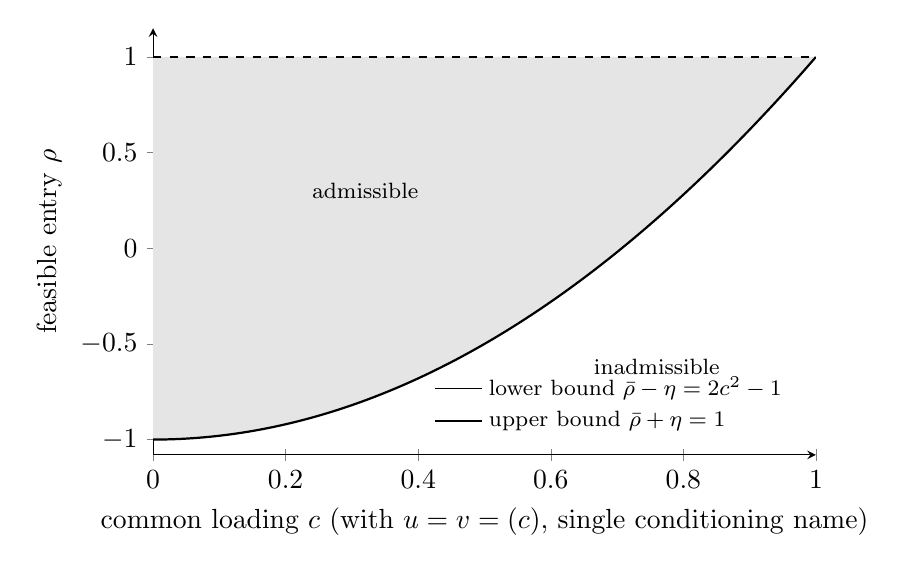
\begin{tikzpicture}
\begin{axis}[
  width=10cm, height=7cm,
  xlabel={common loading $c$ (with $u = v = (c)$, single conditioning name)},
  ylabel={feasible entry $\rho$},
  xmin=0, xmax=1, ymin=-1.08, ymax=1.15,
  axis lines=left,
  ytick={-1,-0.5,0,0.5,1},
  legend cell align=left,
  legend pos=south east,
  legend style={font=\footnotesize, draw=none, fill=none},
]
\addplot[draw=none, fill=gray!20] coordinates {
  (0,-1) (0.05,-0.995) (0.1,-0.98) (0.15,-0.955) (0.2,-0.92)
  (0.25,-0.875) (0.3,-0.82) (0.35,-0.755) (0.4,-0.68) (0.45,-0.595)
  (0.5,-0.5) (0.55,-0.395) (0.6,-0.28) (0.65,-0.155) (0.7,-0.02)
  (0.75,0.125) (0.8,0.28) (0.85,0.445) (0.9,0.62) (0.95,0.805) (1,1)
  (0,1)
} -- cycle;
\addplot[thick, domain=0:1, samples=100] {2*x^2 - 1};
\addlegendentry{lower bound $\bar\rho - \eta = 2c^2 - 1$}
\addplot[thick, dashed, domain=0:1] {1};
\addlegendentry{upper bound $\bar\rho + \eta = 1$}
\node[font=\footnotesize] at (axis cs:0.32,0.30) {admissible};
\node[font=\footnotesize] at (axis cs:0.76,-0.62) {inadmissible};
\end{axis}
\end{tikzpicture}
\caption{The Schur interval \eqref{eq:admiss:interval} for a pair with a
symmetric loading $c$ on a single common conditioning name:
$\bar\rho = c^2$, $\eta = 1 - c^2$, feasible range $[2c^2 - 1,\, 1]$. A
strong common driver never forbids $\rho = 1$, but it progressively
squeezes out anticorrelation: at $c = 0.9$ the pair cannot be quoted below
$0.62$.}
\label{fig:admiss:interval}
\end{figure}

\begin{remark}[Consequences for $\Cega$ bumps]\label{rem:admiss:cega}
$\Cega$ is quoted per correlation point: a bump of $0.01$ in one entry of
$\Omega$. Theorem~\ref{thm:admiss:single} is the statement that this bump
is only well-defined while $\rho \pm 0.01$ stays inside
$[\bar\rho_{ij} - \eta_{ij},\, \bar\rho_{ij} + \eta_{ij}]$. Near the
boundary --- high $\abs{t}$ in \eqref{eq:admiss:param} --- a symmetric
bump exits the elliptope on one side, and the
sensitivity must be computed one-sided, or better, in the coordinate $t$,
which is unconstrained on $(-1, 1)$ and geometry-respecting by
construction.
\end{remark}

\begin{remark}[Conditioning of the fixed block $B$]\label{rem:admiss:Bcond}
Assumption~\ref{ass:admiss:B} excludes \emph{exact} singularity of $B$
only. Near-singularity is not excluded, and it is the operationally
dangerous regime: whenever the rest-of-book correlations crowd upward ---
the ambient market state in exactly the crisis scenarios for which the
stress machinery of Section~\ref{sec:admiss:blend} is designed ---
$\mu_{\min}(B)$ collapses and every quantity built on $B^{-1}$ inflates.
A single rest-of-book pair quoted at $0.99$ already puts $\mu_{\min}(B)$
at order $10^{-2}$ and entries of $B^{-1}$ at order $10^{2}$; the scalars
$q_u$, $q_v$, $\bar\rho_{ij}$ are then differences of $O(10^{2})$
quantities, and the interval endpoints $\bar\rho_{ij} \pm \eta_{ij}$ lose
precision to catastrophic cancellation --- even though the bound itself
remains exact and admissibility of $\Omega$ still guarantees
$q_u \le 1$, $q_v \le 1$. Three implementation rules follow. First, never
form $B^{-1}$ explicitly: compute $q_u$, $q_v$, $\bar\rho_{ij}$ through a
stable factorisation of $B$ (a Cholesky solve). Second, report
$\mu_{\min}(B)$, or the condition number $\kappa(B)$, alongside every
Schur interval, and flag the interval as numerically suspect when
$\kappa(B)$ exceeds the implementation's threshold. Third, the
eigenvalue floor of Remark~\ref{rem:admiss:floor} below conditions the
\emph{modified} block only and never touches $B$; it is no defence
here. The fragility is worst precisely where the tool is most wanted; it
must be surfaced, not assumed away.
\end{remark}

\section{Blockwise modification and conditional correlation}
\label{sec:admiss:block}

The construction now scales from one entry to a whole sub-block. Partition
the names into a block $\mathcal{I}$ to be modified (say, the equities in a
hybrid basket) and its complement $\mathcal{J}$ to be kept exactly as quoted
(say, the FX names, plus every equity--FX cross correlation). After
reordering,
\begin{equation}\label{eq:admiss:blockOmega}
  \Omega \;=\;
  \begin{pmatrix} A & C^{\mathsf T} \\ C & B \end{pmatrix},
  \qquad
  A = \Omega_{\mathcal I \mathcal I}, \quad
  B = \Omega_{\mathcal J \mathcal J}, \quad
  C = \Omega_{\mathcal J \mathcal I},
\end{equation}
with $B \succ 0$ (Assumption~\ref{ass:admiss:B}). The explained/residual
split \eqref{eq:admiss:split} reads
\begin{equation}\label{eq:admiss:APi}
  A \;=\; \Pi + \Sigma_{\mathcal I|\mathcal J},
  \qquad
  \Pi = C^{\mathsf T} B^{-1} C,
  \qquad
  \Sigma_{\mathcal I|\mathcal J} = \SchurC{B}{\Omega} .
\end{equation}

\begin{theorem}[Blockwise modification criterion]\label{thm:admiss:blockmod}
Fix $B \succ 0$ and $C$, and let $A_{\mathrm{new}}$ be symmetric. The
modified matrix
\[
  \Omega_{\mathrm{new}}
  = \begin{pmatrix} A_{\mathrm{new}} & C^{\mathsf T} \\ C & B \end{pmatrix}
\]
is an admissible correlation matrix if and only if
\begin{equation}\label{eq:admiss:newcond}
  \Sigma_{\mathrm{new}} := A_{\mathrm{new}} - \Pi \;\succeq\; 0
  \qquad\text{and}\qquad
  \operatorname{diag}(\Sigma_{\mathrm{new}}) = \mathbf{1} -
  \operatorname{diag}(\Pi) .
\end{equation}
\end{theorem}

\begin{proof}
Since $B$ and $C$ are unchanged, $\Pi$ is unchanged, and
$\SchurC{B}{\Omega_{\mathrm{new}}} = A_{\mathrm{new}} - \Pi =
\Sigma_{\mathrm{new}}$. By Theorem~\ref{thm:admiss:criterion},
$\Omega_{\mathrm{new}} \succeq 0 \iff \Sigma_{\mathrm{new}} \succeq 0$.
The block $B$ keeps its unit diagonal; the unit-diagonal requirement on
$A_{\mathrm{new}}$ is
$\operatorname{diag}(A_{\mathrm{new}}) = \operatorname{diag}(\Pi) +
\operatorname{diag}(\Sigma_{\mathrm{new}}) = \mathbf{1}$, which is the
second condition of \eqref{eq:admiss:newcond}. Symmetry of
$\Omega_{\mathrm{new}}$ is symmetry of $A_{\mathrm{new}}$.
\end{proof}

The freedom left inside the block is therefore exactly: a PSD matrix with a
\emph{prescribed} diagonal. The natural coordinates for that object are a
correlation matrix and a fixed diagonal scaling --- and this is where the
ladder's recursive structure appears: the admissible modifications of a
block of an $n$-name correlation matrix are themselves parametrised by a
smaller correlation matrix.

\begin{definition}[Conditional correlation matrix]\label{def:admiss:condcorr}
Let $\Sigma_{\mathcal I|\mathcal J}$ be as in \eqref{eq:admiss:APi} and
suppose its diagonal entries --- the conditional variances
$D_{ii} = 1 - \Pi_{ii}$ --- are strictly positive. Write
$D := \operatorname{diag}\bigl(\Sigma_{\mathcal I|\mathcal J}\bigr)$ for the
diagonal matrix of conditional variances. The \emph{conditional correlation
matrix} of the block $\mathcal I$ given $\mathcal J$ is
\begin{equation}\label{eq:admiss:R}
  R \;:=\; D^{-1/2}\, \Sigma_{\mathcal I|\mathcal J}\, D^{-1/2}
  \;\in\; \mathcal{E}_{n_{\mathcal I}} .
\end{equation}
It is the correlation matrix of the regression residuals
$X_{\mathcal I} - G X_{\mathcal J}$ of
Proposition~\ref{prop:admiss:condcov}.
\end{definition}

\begin{proposition}[The block's only degree of freedom]
\label{prop:admiss:bijection}
Fix $B \succ 0$ and $C$ with $\Pi_{ii} < 1$ for all $i \in \mathcal I$, and
let $D = \operatorname{diag}(\mathbf{1} - \operatorname{diag}(\Pi))$. The
map
\[
  R \;\longmapsto\;
  A_{\mathrm{new}}(R) \;=\; \Pi + D^{1/2} R\, D^{1/2}
\]
is a bijection between the elliptope $\mathcal{E}_{n_{\mathcal I}}$ and the
set of admissible replacement blocks $A_{\mathrm{new}}$ in
Theorem~\ref{thm:admiss:blockmod}.
\end{proposition}

\begin{proof}
If $R \in \mathcal{E}_{n_{\mathcal I}}$ then $\Sigma_{\mathrm{new}} =
D^{1/2} R D^{1/2}$ is PSD (congruence by the invertible $D^{1/2}$ preserves
positivity) and $(D^{1/2} R D^{1/2})_{ii} = D_{ii} R_{ii} = D_{ii} =
1 - \Pi_{ii}$, so both conditions of \eqref{eq:admiss:newcond} hold.
Conversely, any admissible $A_{\mathrm{new}}$ has $\Sigma_{\mathrm{new}} =
A_{\mathrm{new}} - \Pi \succeq 0$ with
$\operatorname{diag}(\Sigma_{\mathrm{new}}) = \operatorname{diag}(D)$, and
$R = D^{-1/2} \Sigma_{\mathrm{new}} D^{-1/2}$ is PSD with unit diagonal.
The two maps are mutually inverse.
\end{proof}

Everything else --- $B$, $C$, hence $\Pi$, $G$, and $D$ --- is pinned by the
part of the market left untouched. The modeller who wants to
restructure dependence inside a block, without disturbing a single quoted
correlation outside it, has exactly one dial: the conditional correlation
matrix $R$.

\section{Convex blending: stressing a block toward comonotonicity}
\label{sec:admiss:blend}

The canonical application of Proposition~\ref{prop:admiss:bijection} is the
correlation stress: in a crisis scenario the names inside $\mathcal I$
should become more strongly dependent, while the quoted structure of the
rest of the book --- block $B$ and all cross-correlations $C$ --- must be
held exactly at market. The construction is a convex blend of the
conditional correlation matrix toward the comonotone extreme.

\begin{theorem}[Convex blending]\label{thm:admiss:blend}
Let $R_0 \in \mathcal{E}_{n_{\mathcal I}}$ be the initial conditional
correlation matrix \eqref{eq:admiss:R}, and for $\lambda \in [0, 1]$ define
\begin{equation}\label{eq:admiss:blend}
  R(\lambda) \;=\; (1 - \lambda)\, R_0 + \lambda\, \mathbf{1}\mathbf{1}^{\mathsf T},
  \qquad
  A(\lambda) \;=\; \Pi + D^{1/2} R(\lambda)\, D^{1/2},
  \qquad
  \Omega(\lambda) \;=\;
  \begin{pmatrix} A(\lambda) & C^{\mathsf T} \\ C & B \end{pmatrix}.
\end{equation}
Then for every $\lambda \in [0, 1]$, $\Omega(\lambda)$ is an admissible
correlation matrix, it agrees with $\Omega$ outside the block
$\mathcal I \times \mathcal I$, and $\Omega(0) = \Omega$.
\end{theorem}

\begin{proof}
The all-ones matrix $\mathbf{1}\mathbf{1}^{\mathsf T}$ is symmetric, rank
one, with eigenvalues $\{n_{\mathcal I}, 0, \dots, 0\}$, hence PSD, and has
unit diagonal; so it lies in $\mathcal{E}_{n_{\mathcal I}}$. The elliptope
is convex (Definition~\ref{def:admiss:corr}), so
$R(\lambda) \in \mathcal{E}_{n_{\mathcal I}}$ for all $\lambda \in [0,1]$:
explicitly, $x^{\mathsf T} R(\lambda) x = (1-\lambda)\, x^{\mathsf T} R_0 x
+ \lambda\, (\mathbf{1}^{\mathsf T} x)^2 \ge 0$ and
$\operatorname{diag}(R(\lambda)) = (1-\lambda)\mathbf{1} +
\lambda\mathbf{1} = \mathbf{1}$. Proposition~\ref{prop:admiss:bijection}
then delivers admissibility of $\Omega(\lambda)$; blocks $B$ and $C$ are
untouched by construction, and $\lambda = 0$ recovers
$A(0) = \Pi + D^{1/2} R_0 D^{1/2} = \Pi + \Sigma_{\mathcal I|\mathcal J} =
A$.
\end{proof}

As $\lambda \uparrow 1$ the block's residuals become perfectly
conditionally correlated: given the rest of the market, the names in
$\mathcal I$ move as one. The stress is \emph{maximal} in a precise sense
--- $\lambda = 1$ puts $R$ at the comonotone vertex
$\mathbf{1}\mathbf{1}^{\mathsf T}$, a rank-one point of the elliptope's
boundary, and in fact an extreme point: a rank-$r$ correlation matrix is
an extreme point of $\mathcal{E}_n$ exactly when $r(r+1)/2 \le n$ (Grone,
Pierce \& Watkins, \emph{Extremal correlation matrices}, Linear Algebra
Appl.\ 134 (1990), 63--70), and rank one always qualifies --- and
\emph{surgical} in an equally precise sense: no quoted correlation outside
the block moves at all.

\begin{example}[Blending traverses the Schur interval]
\label{ex:admiss:blendtraverse}
Return to Example~\ref{ex:admiss:threename} with $\mathcal I = \{1, 2\}$,
$\mathcal J = \{3\}$, and take the initially quoted pair correlation to be
exactly the explained centre, $\rho_{12} = \bar\rho_{12} = 0.30$. Then
\[
  \Pi = \begin{pmatrix} 0.36 & 0.30 \\ 0.30 & 0.25 \end{pmatrix},
  \qquad
  \Sigma_{\mathcal I|\mathcal J}
  = A - \Pi
  = \begin{pmatrix} 0.64 & 0 \\ 0 & 0.75 \end{pmatrix},
  \qquad
  D = \begin{pmatrix} 0.64 & 0 \\ 0 & 0.75 \end{pmatrix},
  \qquad
  R_0 = \mathrm{Id}_2 :
\]
the two names are conditionally \emph{uncorrelated} given name 3; their
entire quoted correlation of $0.30$ is explained through the common name.
Blending per \eqref{eq:admiss:blend} gives
$R(\lambda) = \bigl(\begin{smallmatrix} 1 & \lambda \\ \lambda & 1
\end{smallmatrix}\bigr)$, so
\[
  \bigl(D^{1/2} R(\lambda) D^{1/2}\bigr)_{12}
  = \lambda \sqrt{0.64 \times 0.75} = 0.6928\,\lambda,
  \qquad
  A(\lambda)_{12} = 0.30 + 0.6928\,\lambda .
\]
The blend traverses exactly the upper half of the Schur interval of
Example~\ref{ex:admiss:threename}, with $\lambda$ coinciding with the
partial-correlation coordinate $t$ of
Corollary~\ref{cor:admiss:partial}; at $\lambda = 1$ the quoted pair
correlation reaches the boundary value $0.9928$ and $\Omega(1)$ is
singular. The single-entry bound and the block blend are one construction
seen at two scales.
\end{example}

\subsection{Approach to singularity and the choice of $\lambda$}
\label{sec:admiss:singularity}

The comonotone extreme $\mathbf{1}\mathbf{1}^{\mathsf T}$ has rank one, so
if $R_0 \succ 0$ and $\lambda$ is close to $1$, the blend $R(\lambda)$ is
close to rank one and the conditional covariance
$D^{1/2} R(\lambda) D^{1/2}$ is nearly singular. $\Omega(\lambda)$ remains
admissible --- Theorem~\ref{thm:admiss:blend} is uniform on $[0,1]$ --- but
it may cease to be \emph{positive definite}, and with it go the precision
matrix, the Gaussian density, and the Cholesky factor a Monte Carlo engine
needs.

\begin{example}[Equicorrelated block: exact eigenvalues along the blend]
\label{ex:admiss:eigen}
Let $R_0$ be equicorrelated on $n_{\mathcal I} = 3$ names with common
conditional correlation $r = 0.4$. An equicorrelated matrix with parameter
$r$ has eigenvalues $1 + (n_{\mathcal I} - 1) r$ (eigenvector
$\mathbf{1}$) and $1 - r$ (multiplicity $n_{\mathcal I} - 1$). Blending
preserves equicorrelation with parameter $r(\lambda) = (1 - \lambda) r +
\lambda = 0.4 + 0.6 \lambda$, so
\[
  \mu_{\max}\bigl(R(\lambda)\bigr) = 1 + 2\, r(\lambda) = 1.8 + 1.2\lambda,
  \qquad
  \mu_{\min}\bigl(R(\lambda)\bigr) = 1 - r(\lambda) = 0.6\, (1 - \lambda),
\]
the latter with multiplicity two. The smallest eigenvalue decays
\emph{linearly} to zero: at $\lambda = 1$ the spectrum is $\{3, 0, 0\}$,
the rank-one comonotone limit. The linear decay to zero is generic, not an
artefact of equicorrelation: for any $R_0 \succ 0$,
$R(\lambda) \succeq (1 - \lambda) R_0$ gives
$\mu_{\min}(R(\lambda)) \ge (1 - \lambda)\, \mu_{\min}(R_0)$. For the
matching upper bound, write $R(\lambda) = M_0 + w w^{\mathsf T}$ with
$M_0 = (1 - \lambda) R_0$ and $w = \sqrt{\lambda}\, \mathbf{1}$: the
interlacing theorem for a rank-one positive-semidefinite update states
$\mu_{\min}(M_0 + w w^{\mathsf T}) \le \mu_2(M_0)$, where $\mu_2$ denotes
the second-smallest eigenvalue (Horn \& Johnson, \emph{Matrix Analysis},
2nd ed., Corollary~4.3.9), and $\mu_2(M_0) = (1 - \lambda)\, \mu_2(R_0)$,
so $\mu_{\min}(R(\lambda)) \le (1 - \lambda)\, \mu_{2}(R_0)$. The smallest
eigenvalue is thus pinched between two linear functions of $(1 - \lambda)$
and vanishes at $\lambda = 1$ exactly to first order; the closed-form
floor $(1 - \lambda)\, \mu_{\min}(R_0)$ is available for any block. As a
consistency check, when $\mu_{\min}(R_0)$ has multiplicity at least two,
$\mu_2(R_0) = \mu_{\min}(R_0)$, the two bounds coincide, and
$\mu_{\min}(R(\lambda)) = (1 - \lambda)\, \mu_{\min}(R_0)$ exactly ---
which is precisely the equicorrelated computation above (multiplicity
$n_{\mathcal I} - 1 = 2$).
\end{example}

\begin{figure}[ht]
\centering
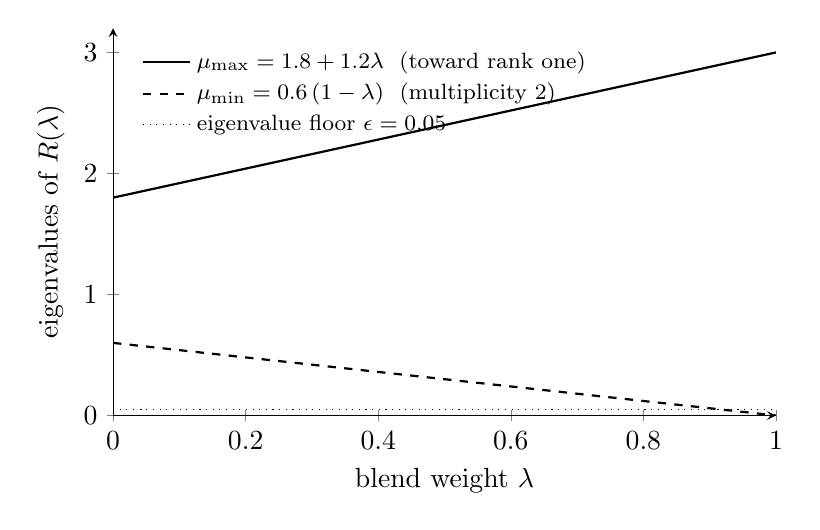
\begin{tikzpicture}
\begin{axis}[
  width=10cm, height=6.5cm,
  xlabel={blend weight $\lambda$},
  ylabel={eigenvalues of $R(\lambda)$},
  xmin=0, xmax=1, ymin=0, ymax=3.2,
  axis lines=left,
  legend cell align=left,
  legend pos=north west,
  legend style={font=\footnotesize, draw=none, fill=none},
]
\addplot[thick, domain=0:1] {1.8 + 1.2*x};
\addlegendentry{$\mu_{\max} = 1.8 + 1.2\lambda$ \ (toward rank one)}
\addplot[thick, dashed, domain=0:1] {0.6*(1 - x)};
\addlegendentry{$\mu_{\min} = 0.6\,(1 - \lambda)$ \ (multiplicity 2)}
\addplot[dotted, domain=0:1] {0.05};
\addlegendentry{eigenvalue floor $\epsilon = 0.05$}
\end{axis}
\end{tikzpicture}
\caption{Spectrum of the blended conditional correlation matrix of
Example~\ref{ex:admiss:eigen} ($n_{\mathcal I} = 3$, $r = 0.4$). The
smallest eigenvalue decays linearly to zero; a floor $\epsilon$ caps the
usable stress at $\lambda^\ast = 1 - \epsilon / (1 - r)$, here
$\lambda^\ast \approx 0.917$. This $\lambda^\ast$ floors the \emph{bare}
conditional correlation $R(\lambda)$ only and is illustrative; the object
a Monte Carlo engine Cholesky-factorises is $\Omega(\lambda)$, whose
operational floor is the $\mu_{\min}(D)$-weighted cap of
Remark~\ref{rem:admiss:floor}.}
\label{fig:admiss:eigen}
\end{figure}

\begin{remark}[Practical selection of the blend weight]
\label{rem:admiss:floor}
When strict positive definiteness of $\Omega(\lambda)$ is required (an
invertible covariance, a Cholesky factorisation, a well-conditioned
precision matrix), impose an eigenvalue floor $\epsilon > 0$. Two floors
must be distinguished, because they are not equivalent.

\emph{Conditional-covariance floor:} require
$\mu_{\min}\bigl(D^{1/2} R(\lambda) D^{1/2}\bigr) \ge \epsilon$. Here a
conservative closed-form cap is available, from two one-line
inequalities. First, $R(\lambda) \succeq (1 - \lambda) R_0$ (the omitted
term $\lambda\, \mathbf{1}\mathbf{1}^{\mathsf T}$ is PSD), so
$\mu_{\min}(R(\lambda)) \ge (1 - \lambda)\, \mu_{\min}(R_0)$. Second, for
any unit vector $x$,
$x^{\mathsf T} D^{1/2} R D^{1/2} x \ge
\mu_{\min}(R)\, \bigl\| D^{1/2} x \bigr\|^2 \ge
\mu_{\min}(R)\, \mu_{\min}(D)$, so
$\mu_{\min}\bigl(D^{1/2} R D^{1/2}\bigr) \ge
\mu_{\min}(D)\, \mu_{\min}(R)$. Chaining the two, the floor holds whenever
$\lambda \le 1 - \epsilon / \bigl(\mu_{\min}(D)\, \mu_{\min}(R_0)\bigr)$.
This cap is scoped to the conditional-covariance floor and to it alone.

\emph{$\Omega$-level floor:} require
$\mu_{\min}(\Omega(\lambda)) \ge \epsilon$ --- this is the floor the
Monte Carlo engine actually needs, since $\Omega(\lambda)$ is the matrix
it Cholesky-factorises. The cap above does \emph{not} deliver it: the
congruence of Lemma~\ref{lem:admiss:congruence} preserves inertia, not
eigenvalues, so $\mu_{\min}(\Omega(\lambda))$ can lie far below
$\mu_{\min}\bigl(\Sigma(\lambda) \oplus B\bigr)$ with
$\Sigma(\lambda) = D^{1/2} R(\lambda) D^{1/2}$. What the congruence does
give (Ostrowski's theorem on congruence transformations) is the corrected
bound
\[
  \mu_{\min}\bigl(\Omega(\lambda)\bigr)
  \;\ge\;
  \sigma_{\min}(L)^2 \cdot
  \min\bigl(\mu_{\min}(\Sigma(\lambda)),\; \mu_{\min}(B)\bigr),
\]
with $L$ the unit-triangular factor of \eqref{eq:admiss:ldl} (fixed along
the blend, since $B$ and $C$ are). Since $\sigma_{\min}(L)$ must itself be
computed, an implementation either uses this corrected bound or ---
simpler, and recommended --- checks $\mu_{\min}(\Omega(\lambda))$ (or the
Cholesky factorisation of $\Omega(\lambda)$) directly at the target
$\lambda$, backtracking $\lambda$ toward zero until the floor is restored.

The floor $\epsilon$ is a numerical-conditioning parameter of the
implementation, not of the theory: every $\lambda \in [0, 1]$ is
admissible in exact arithmetic.
\end{remark}

\section{Why not global partial correlations}\label{sec:admiss:global}

Corollary~\ref{cor:admiss:partial} suggests a tempting alternative: since
the partial correlations $\rho_{ij \cdot \mathcal{R}}$ are each free in
$[-1, 1]$, stress dependence by editing the global
partial-correlation matrix
\[
  P_{ij} \;=\; -\frac{\Theta_{ij}}{\sqrt{\Theta_{ii}\, \Theta_{jj}}},
  \qquad \Theta = \Omega^{-1},
\]
and mapping back to $\Omega$.

The obstruction is locality. The map from $P$ back to $\Omega$ runs through
a matrix inversion, and inversion is a \emph{global} operation: perturbing
even a single entry $P_{ij}$ with $i, j \in \mathcal I$ changes, in
general, \emph{every} entry of the reconstructed $\Omega$ --- including the
block $B$ and the cross-block $C$ that the mandate requires held at
market. (This is visible already in Proposition~\ref{prop:admiss:blockinv}:
the $\mathcal I \times \mathcal I$ block of $\Theta$ is
$\Sigma_{\mathcal I|\mathcal J}^{-1}$, which entangles $A$, $B$, and $C$;
inverting a modified $\Theta$ redistributes the change across all three.)
Partial-correlation coordinates are the right chart for checking
admissibility of a \emph{given} matrix and for one-entry moves; they are
the wrong chart for constrained blockwise modification. The Schur-based
construction of Sections~\ref{sec:admiss:block}--\ref{sec:admiss:blend}
exists precisely because it localises: it fixes $B$ and $C$ \emph{exactly},
by construction, and exposes the residual freedom in coordinates ($R$)
where admissibility is manifest.

\section{Closing the ladder}\label{sec:admiss:closing}

The three rungs now stand in one pattern. At rungs 2 and 3, admissibility
is positive semidefiniteness of a conditional object and the boundary of
the feasible set is its loss of rank; at rung 1 the feasible set is a
different convex cone, and the correspondence is one of shape, not an
identity:

\begin{itemize}
  \item \emph{One name.} The density constraint of Volume~I, Chapter~2 has
        the same shape one level down: the feasible set is the cone of
        \emph{nonnegative measures} (risk-neutral densities), and the
        no-butterfly condition --- convexity of the call price $C(K,T)$ in
        $K$ --- is nonnegativity of a \emph{linear} functional of the
        density (the price of the butterfly portfolio), not of a quadratic
        form. The cone of nonnegative measures is not the PSD cone, and no
        identity between the rungs is claimed; the shared shape is a convex
        cone constraint whose boundary is degeneracy --- loss of mass of
        the density at rung 1, loss of rank of the matrix at rungs 2
        and 3.
  \item \emph{Two names.} $\abs{\rho} \le 1$ is
        Theorem~\ref{thm:admiss:single} with an empty conditioning set
        (Remark~\ref{rem:admiss:rung2}); its upper boundary $\rho = 1$ is
        $\xi = 0$, the collapse of the basket vol spread
        $\xi = \sbmean - \sB$ of Chapter~1. Admissibility is also what
        keeps the Margrabe volatility of Chapter~3 real: for
        $\rho \in [-1, 1]$,
        $\SigmaM^2 = \sigma_1^2 + \sigma_2^2 - 2\rho\sigma_1\sigma_2
        = (\sigma_1 - \sigma_2)^2 + 2 \sigma_1 \sigma_2 (1 - \rho) \ge 0$,
        with equality only at $\rho = 1$, $\sigma_1 = \sigma_2$.
  \item \emph{$n$ names.} $\Omega \in \mathcal{E}_n$, certified blockwise
        by Theorem~\ref{thm:admiss:criterion}, moved one entry at a time
        within the Schur interval \eqref{eq:admiss:interval}, and stressed
        one block at a time by the blend \eqref{eq:admiss:blend} ---
        without ever leaving the elliptope, and without touching what was
        quoted outside the block.
\end{itemize}

Two forward couplings deserve to be stated explicitly, because they connect
this static chapter to the dynamics of Chapter~2.

\begin{remark}[Admissibility under the quoting conventions]
\label{rem:admiss:sticky}
The entries of $\Omega$ do not sit still: the constituent volatilities are
the per-name ATM vols $\satmi{i}(\lFi{i}, T)$ of constraint C1, and as
the forwards move, the vols move. Under \stickyrho{} the correlation is
held fixed, $\dd\rho = 0$, and admissibility of $\Omega$ is a static check.
Under \stickycvc{} the correlation is the determined function
$\rho(\sigma_1, \sigma_2, \xi)$ --- the spread $\xi$ is held invariant and
$\rho$ moves with the vols, which is exactly what generates the shadow
Greeks of Chapter~2. Every convention-induced correlation path
$\rho(\cdot)$ must remain inside the Schur interval
\eqref{eq:admiss:interval} \emph{given the contemporaneous rest of the
matrix}: the interval is not static --- under a book-wide convention the
bounds $\bar\rho_{ij}$ and $\eta_{ij}$ are themselves functions of the
instantaneous $u$, $v$, $B$, which co-move with the pair being tracked as
the vols move --- so the check is pointwise in time, with every quantity
evaluated on the same instant's matrix. For a pair embedded in an
$n$-name book, the binding constraint on a \stickycvc{}-driven correlation
move is $\rho \le \bar\rho_{ij} + \eta_{ij}$, and the ceiling obeys
\[
  \bar\rho_{ij} + \eta_{ij} \;\le\; 1 \qquad\text{always},
\]
by two applications of Cauchy--Schwarz:
$\bar\rho_{ij} = u^{\mathsf T} B^{-1} v \le \sqrt{q_u q_v}$
(Cauchy--Schwarz in the $B^{-1}$ inner product), and
$\sqrt{q_u q_v} + \sqrt{(1 - q_u)(1 - q_v)} \le
\sqrt{(q_u + 1 - q_u)(q_v + 1 - q_v)} = 1$ (Cauchy--Schwarz in
$\mathbb{R}^2$ applied to $(\sqrt{q_u}, \sqrt{1 - q_u})$ and
$(\sqrt{q_v}, \sqrt{1 - q_v})$). Equality throughout holds if and only if
$u = v$: the first inequality is tight iff $u$ and $v$ are positively
parallel in the $B^{-1}$ geometry, the second iff $q_u = q_v$, and
together these force $u = v$. So the Schur ceiling is \emph{weakly}
tighter than the two-name bound $\rho \le 1$, and strictly tighter exactly
when the two names load \emph{asymmetrically} on the rest of the book
($u \ne v$). $\eta_{ij} < 1$ is \emph{not} the trigger: for
symmetric loadings $u = v$ the ceiling is
$q_u + (1 - q_u) = 1$ exactly, however strong the common loading ---
consistent with Figure~\ref{fig:admiss:interval}, whose upper bound is
identically $1$. Finally, this pointwise check does not settle
admissibility of the full book-wide \stickycvc{} \emph{path}, with all
entries of $\Omega$ moving simultaneously as the vols move: that is a
coupled dynamic question, open at the level of this static chapter and
deferred to the dynamics of Chapter~2. The two-name bound of Chapter~1 is
the correct constraint only for a two-name book.
\end{remark}

\begin{remark}[The same identity, one chapter earlier]
\label{rem:admiss:kalman}
Proposition~\ref{prop:admiss:condcov} is the workhorse of the Bayesian
calibration engine of Volume~I, Chapter~4, in different clothing: there the
joint Gaussian vector is (parameters, observations), the regression matrix
$G$ is the gain applied to the innovation $e_t$, and the posterior
covariance of the parameter ket is the Schur complement of the observation
block in the joint covariance. Conditioning shrinks covariance by the
explained part $\Pi$ --- whether what is being conditioned is a block of
names in a correlation matrix or a vector of smile parameters given a day's
quotes. The ladder of this chapter and the filter of that one are the same
piece of Gaussian linear algebra.
\end{remark}

The admissibility theory of the corpus is now closed: densities
nonnegative and total variance calendar-monotone on every single-name
surface, $\xi \ge 0$ on every pair, and
$\Omega \succeq 0$ --- blockwise certified, boundary understood, and
stressable without leaving the feasible set --- on the full book.
%% ============================================================================
%% frag_volII_ch5.tex -- Vol II, Chapter 5
%% Numerical Methods: Regression Monte Carlo, Control Variates, and Surrogate
%% Pricing (as THEORY).
%% Author: KARPATHY. Governed by NOTATION_CONTRACT.md; macros from
%% build/preamble.tex. First-version voice. No code.
%% Source distilled: LaTex/ControlVariate.tex, informed (never reproduced) by the
%% Python engine (generic_option_gp_pricer.py, mc_analysis_2d.py, monte_carlo_2d.py,
%% montecarlo_payoffs.py). Worked numbers recomputed here; every constant-vol
%% number is flagged per constraint C4, every F=S collapse flagged per Sec.1.2.
%% ============================================================================

\chapter{Numerical Methods: Regression Monte Carlo, Control Variates, and Surrogate Pricing}
\label{chap:numerics}

Every price in this corpus so far has been either a closed form or the solution
of a well-posed differential equation. This chapter treats the remaining case:
a payoff whose price is available only as an expectation, estimated by
simulation. The engineering question is not \emph{how to simulate} --- the Euler
scheme with It\^o correction carries the two-asset dynamics ---
but \emph{how to spend a finite simulation budget so that the estimator is
accurate}. The answer developed here is compositional: a complex payoff is
never priced from scratch. It is priced \emph{relative to a library of simpler
instruments whose prices are already known}, and only the residual is
simulated --- a random variable engineered to be small, smooth, and cheap to
learn.

The mathematics is elementary and is proved in full. The variance-reduction
step is an orthogonal projection in $L^2$; the regularisation of that projection
is the same conjugate Gaussian update that calibrates the single-name volatility
surface in Volume~I; and the surrogate that interpolates the residual across
states is Gaussian-process regression, the nonparametric limit of that same
Bayesian regression. Three ideas, one spine: \emph{represent, regress,
interpolate.}

\begin{remark}[Local notation for this chapter]\label{rem:num:notation}
This chapter introduces symbols scoped to it. Several reuse glyphs owned by the
contract table; each such reuse is \emph{declared here explicitly}
(Convention~3(a)) and is local to this chapter. The number of simulated paths is
$N_{\mathrm{p}}$; the number of state points on a training grid is $N_{x}$; the
number of hedge instruments is $H$. The Monte Carlo path index is
$p = 1,\dots,N_{\mathrm{p}}$ --- \emph{not} the retired $k$, which is not used as an
index (ruling R3); the hedge index is $i = 1,\dots,H$; the state-grid index is
$j = 1,\dots,N_{x}$. A bare $N$ is never written for a count: $\ncdf(\cdot)$ is the
standard normal CDF (ruling R5), and it alone owns that glyph.

The hedge payoffs are written $g_1,\dots,g_H$ --- \emph{not} $h_i$, reserved by
the contract for the Epanechnikov kernel bandwidth (owner I.2); the stencil bump
of Section~\ref{sec:num:example} is $b_x$, for the same reason. The hedge-ratio
vector is $\lambda \in \mathbb{R}^H$, accompanied by a regression intercept
$\lambda_0$. The Gaussian-process covariance function is $\mathcal{K}(\cdot,\cdot)$
and its query cross-covariance vector is $\boldsymbol{\kappa}_\ast$ (not $k_\ast$,
so that $k$ genuinely never reappears); its signal amplitude is $a_{\mathrm{gp}}$
--- distinct from the Margrabe argument $a$ (owner II.3, used unaltered in
Remark~\ref{rem:num:atmspread}) --- and its per-coordinate length scales are
$\ell_{\mathrm{gp},d}$, distinct from the surface coordinate $\lF = \ln(F/\Fref)$.
The GP posterior variance is $v_{\mathrm{GP}}$, written with a $v$ because
$\sigma$ is reserved for implied volatility; the Gaussian-regression noise scale
is $\varsigma$ (not $s$, reserved for the smile skew $s(m)$), and the Monte~Carlo
observation noise on the training grid is $\zeta_j$. Network weights are written
$w$, not $\theta$ (reserved for the Black--Scholes theta, owner I.1, which does
not appear in this chapter). The diagonal training anchors of
Example~\ref{ex:num:gpdesign} are $S_q$, never $S_0$ (a retired, banned pivot
glyph, Convention~7 / ruling R1).

The probability measure is $\mathbb{Q}$ and $L^2(\mathbb{Q})$ denotes the
space of square-integrable payoffs; the sample space is \emph{not} named, since
its usual glyph $\Omega$ is reserved by the contract for the $n$-name
correlation matrix (owner II.4). Inner products of random variables are written as expectations,
$\E[UV]$, never in bra-ket: the bra-ket $\ket{\cdot}$, $\bra{\cdot}$, $\Phi$ is
reserved for the feature/parameter calibration block of Volume~I (Convention~6).
\end{remark}

\section{The pricing problem as an estimation problem}
\label{sec:num:setup}

Fix the risk-neutral filtered probability space carrying the measure
$\mathbb{Q}$ and filtration $\{\mathcal{F}_t\}$ (its sample space is left
unnamed, per Remark~\ref{rem:num:notation}), under the standing assumption of
zero rates and zero dividends, so the discount factor is unity and every forward
equals its spot at the horizon it is read: $F = S$ (flagged here at its first
use; it recurs throughout and is flagged again at each point where it does
analytic work, including in Section~\ref{sec:num:worstof}). Let
$x_0$ denote the current market state --- spots, and the volatility-surface and
correlation parameters that the dynamics of Volumes~I and~II consume.

\begin{definition}[Target and hedge payoffs]\label{def:num:payoffs}
Let $P \in L^2(\mathbb{Q})$ be the discounted terminal payoff of the instrument
to be priced, and let $g_1,\dots,g_H \in L^2(\mathbb{Q})$ be the discounted
terminal payoffs of a \emph{hedge library}: instruments whose arbitrage-free
prices
\[
   \mathrm{Price}(g_i; x_0) \;=\; \E[g_i \mid X_0 = x_0], \qquad i = 1,\dots,H,
\]
are known to high accuracy from a closed form, a PDE solve, or an independent
converged simulation. The object required is
$\mathrm{Price}(P; x_0) = \E[P \mid X_0 = x_0]$. When a library price is itself
only an approximation --- as the basket leg of Section~\ref{sec:num:example}
will be --- unbiasedness holds only \emph{relative to the plugged-in price}; the
resulting bias is isolated in Remark~\ref{rem:num:pricebias}.
\end{definition}

Square-integrability is the only regularity needed: it makes $P$ and the $g_i$
vectors in the Hilbert space $L^2(\mathbb{Q})$ with inner product $\E[UV]$ and it
guarantees the projection of Section~\ref{sec:num:cv} exists and is unique.

\begin{definition}[Crude Monte Carlo estimator]\label{def:num:crude}
Simulate $N_{\mathrm{p}}$ independent paths from $x_0$ and record the pathwise payoffs
$P^{(p)}$, $p = 1,\dots,N_{\mathrm{p}}$. The crude estimator is the sample mean
$\bar P = N_{\mathrm{p}}^{-1}\sum_{p} P^{(p)}$. It is unbiased with
\[
   \Var(\bar P) \;=\; \frac{\Var(P)}{N_{\mathrm{p}}},
   \qquad
   \text{standard error} \;=\; \frac{\sqrt{\Var(P)}}{\sqrt{N_{\mathrm{p}}}}.
\]
\end{definition}

The $N_{\mathrm{p}}^{-1/2}$ law is the entire economic problem. Halving the standard error
costs four times the paths. For a payoff with large $\Var(P)$ --- a spread or
worst-of option, whose value is a thin sliver of a large gross exposure --- the
constant $\sqrt{\Var(P)}$ is punishing. Every method in this chapter attacks
that constant, never the exponent.

\section{Control variates as orthogonal projection}
\label{sec:num:cv}

\subsection{The estimator and its unbiasedness}

\begin{definition}[Control-variate estimator]\label{def:num:cvest}
Given a hedge-ratio vector $\lambda \in \mathbb{R}^H$, define the
\emph{residual} random variable
\begin{equation}\label{eq:num:residual}
   R \;=\; R(\lambda) \;:=\; P - \sum_{i=1}^{H} \lambda_i\, g_i
   \;=\; P - \lambda^{\mathsf T} g ,
\end{equation}
and the control-variate estimator
\begin{equation}\label{eq:num:cvest}
   \widehat{\mathrm{Price}}(P; x_0)
   \;:=\;
   \bar R \;+\; \sum_{i=1}^{H} \lambda_i \, \mathrm{Price}(g_i; x_0),
   \qquad
   \bar R = \frac{1}{N_{\mathrm{p}}}\sum_{p=1}^{N_{\mathrm{p}}} R^{(p)},
\end{equation}
where $R^{(p)} = P^{(p)} - \lambda^{\mathsf T} g^{(p)}$ is the pathwise residual.
\end{definition}

\begin{proposition}[Unbiasedness for every $\lambda$]\label{prop:num:unbiased}
For any fixed $\lambda \in \mathbb{R}^H$, the estimator \eqref{eq:num:cvest} is
unbiased: $\E[\widehat{\mathrm{Price}}(P;x_0)] = \mathrm{Price}(P;x_0)$.
\end{proposition}

\begin{proof}
Taking risk-neutral expectations of \eqref{eq:num:residual},
$\E[R] = \E[P] - \sum_i \lambda_i \E[g_i] = \mathrm{Price}(P;x_0) - \sum_i \lambda_i
\mathrm{Price}(g_i;x_0)$. The sample mean $\bar R$ is unbiased for $\E[R]$, and the
second term of \eqref{eq:num:cvest} is the deterministic constant
$\sum_i \lambda_i \mathrm{Price}(g_i;x_0)$. Adding the two recovers $\mathrm{Price}(P;x_0)$.
\end{proof}

Proposition~\ref{prop:num:unbiased} is the load-bearing fact, with one caveat it
makes explicit: it charges the second term of \eqref{eq:num:cvest} with the
\emph{exact} hedge price $\E[g_i \mid X_0 = x_0]$. Because the hedge prices are
\emph{known}, subtracting the hedges in simulation and adding them back
analytically changes the variance of the estimator but never its mean;
$\lambda$ may therefore be chosen purely to minimise variance. If instead an
approximate price $\widetilde{\mathrm{Price}}(g_i;x_0)$ is plugged in, the estimator
acquires a deterministic bias
$\sum_i \lambda_i\bigl(\widetilde{\mathrm{Price}}(g_i;x_0) - \E[g_i\mid X_0=x_0]\bigr)$
that does \emph{not} shrink with $N_{\mathrm{p}}$; this is the subject of
Remark~\ref{rem:num:pricebias}.

\subsection{The variance-optimal hedge ratio}

Write $\tilde U := U - \E[U]$ for the centring of a random variable, and let
\[
   \Sigma_{gg} := \Cov(g) \in \mathbb{R}^{H\times H},
   \qquad
   \Sigma_{gP} := \Cov(g, P) \in \mathbb{R}^{H},
\]
with entries $(\Sigma_{gg})_{i\ell} = \Cov(g_i, g_\ell)$ and
$(\Sigma_{gP})_i = \Cov(g_i, P)$.

\begin{theorem}[Optimal control variate as $L^2$ projection]\label{thm:num:proj}
Suppose $\Sigma_{gg}$ is nonsingular. Then
\[
   \lambda^\star \;=\; \arg\min_{\lambda \in \mathbb{R}^H}
     \Var\!\bigl(P - \lambda^{\mathsf T} g\bigr)
\]
exists, is unique, and is the solution of the normal equations
\begin{equation}\label{eq:num:normal}
   \Sigma_{gg}\, \lambda^\star \;=\; \Sigma_{gP},
   \qquad\text{i.e.}\qquad
   \lambda^\star = \Sigma_{gg}^{-1}\Sigma_{gP}.
\end{equation}
The optimal residual $R^\star = P - \lambda^{\star\mathsf T} g$ is
\emph{uncorrelated with every hedge}: $\Cov(g_i, R^\star) = 0$ for all $i$.
Its variance is
\begin{equation}\label{eq:num:varred}
   \Var(R^\star) \;=\; \Var(P) - \Sigma_{gP}^{\mathsf T}\Sigma_{gg}^{-1}\Sigma_{gP}
   \;=\; \Var(P)\,\bigl(1 - \varrho^2\bigr),
\end{equation}
where
$\varrho^2 := \Sigma_{gP}^{\mathsf T}\Sigma_{gg}^{-1}\Sigma_{gP}/\Var(P) \in [0,1]$
is the squared multiple correlation between $P$ and the hedge span. (The
symbol is $\varrho$, not $\rho$: $\rho$ is reserved for pairwise asset
correlation.) Both $\lambda^\star$ and $\varrho^2$ depend on
$P$ and $g$ only through their \emph{centred} second moments, so the optimum is
invariant to any additive constant --- the reason the empirical fit below must
carry an intercept.
\end{theorem}

\begin{proof}
The map $\lambda \mapsto \Var(\tilde P - \lambda^{\mathsf T}\tilde g) =
\Var(P) - 2\lambda^{\mathsf T}\Sigma_{gP} + \lambda^{\mathsf T}\Sigma_{gg}\lambda$
is a quadratic form with Hessian $2\Sigma_{gg}$, positive definite by
hypothesis, hence strictly convex with a unique stationary point. Setting the
gradient $-2\Sigma_{gP} + 2\Sigma_{gg}\lambda$ to zero gives
\eqref{eq:num:normal}. Orthogonality is the stationarity condition read
componentwise: $\Cov(g_i, R^\star) = (\Sigma_{gP} - \Sigma_{gg}\lambda^\star)_i =
0$. Substituting $\lambda^\star$ into the quadratic form yields
\eqref{eq:num:varred}. Geometrically, $\sum_i \lambda^\star_i \tilde g_i$ is the
orthogonal projection of $\tilde P$ onto the closed subspace
$\mathrm{span}\{\tilde g_1,\dots,\tilde g_H\} \subset L^2(\mathbb{Q})$,
and $\tilde R^\star = \tilde P - \mathrm{proj}\,\tilde P$ is the projection
residual, orthogonal to the subspace by construction --- the Hilbert-space
Pythagorean identity \eqref{eq:num:varred}.
\end{proof}

Figure~\ref{fig:num:projection} is the whole theorem in one picture: $P$ is a
vector, the hedges span a plane, and the crude estimator wastes its budget on
the part of $P$ that already lies in the plane --- the part whose expectation is
known exactly and for free.

\begin{figure}[t]
\centering
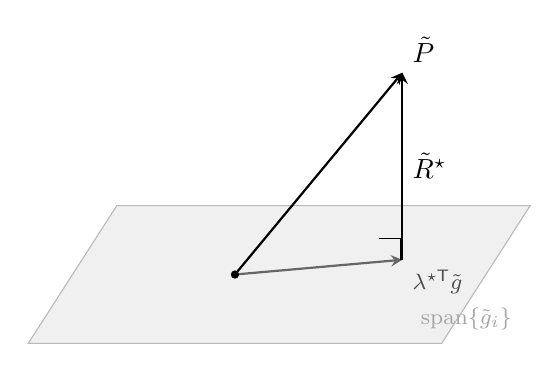
\begin{tikzpicture}[scale=1.25,>=stealth]
  % the hedge span (a plane, drawn as a parallelogram)
  \fill[gray!12] (-2.1,-0.7) -- (2.1,-0.7) -- (3.0,0.7) -- (-1.2,0.7) -- cycle;
  \draw[gray!55] (-2.1,-0.7) -- (2.1,-0.7) -- (3.0,0.7) -- (-1.2,0.7) -- cycle;
  \node[gray!70] at (2.35,-0.45) {\footnotesize $\mathrm{span}\{\tilde g_i\}$};
  % projection point
  \coordinate (O) at (0,0);
  \coordinate (Pp) at (1.7,0.15);   % projection of P onto the plane
  \coordinate (P)  at (1.7,2.05);   % P itself
  % vectors
  \draw[->,thick] (O) -- (P)  node[above right] {$\tilde P$};
  \draw[->,thick,black!60] (O) -- (Pp) node[below right,black!70]
        {\footnotesize $\lambda^{\star\mathsf T}\tilde g$};
  \draw[->,thick] (Pp) -- (P) node[midway,right] {$\tilde R^\star$};
  % right-angle marker
  \draw (Pp) ++(-0.02,0.0) -- ++(0,0.22) -- ++(-0.22,0);
  \fill (O) circle (1.2pt);
\end{tikzpicture}
\caption{Control variate as orthogonal projection in $L^2(\mathbb{Q})$.
The residual $\tilde R^\star$ is orthogonal to the hedge span; by
\eqref{eq:num:varred} its length squared is $\Var(P)(1-\varrho^2)$. Simulation
is spent only on $\tilde R^\star$, the component of $P$ that the known hedge
prices cannot already supply.}
\label{fig:num:projection}
\end{figure}

\begin{corollary}[Variance-reduction budget]\label{cor:num:budget}
Under \eqref{eq:num:varred}, the paths required to reach a fixed standard error
scale by the factor $1-\varrho^2$ relative to crude Monte Carlo. A hedge span
capturing $\varrho^2 = 0.99$ of the variance of $P$ cuts the path count by a
factor of $100$ at equal accuracy.
\end{corollary}

This is the ``core efficiency gain'': the residual $R^\star$ converges rapidly
in $N_{\mathrm{p}}$ precisely because its variance has been contracted by $1-\varrho^2$
before a single path is averaged. Figure~\ref{fig:num:varred} plots the budget
factor.

\begin{figure}[t]
\centering
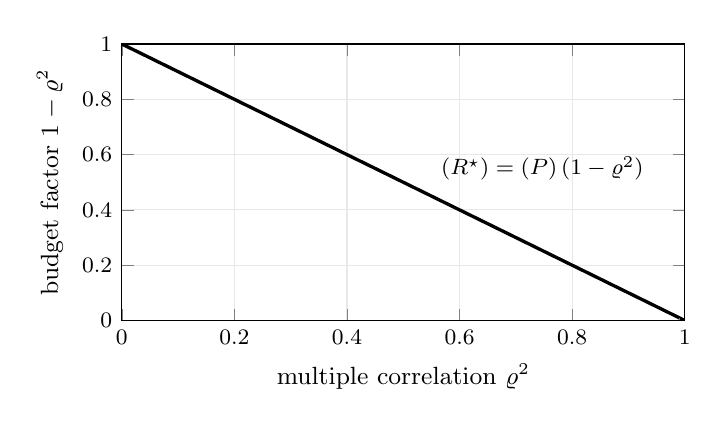
\begin{tikzpicture}
\begin{axis}[
    width=0.72\textwidth, height=0.42\textwidth,
    xlabel={multiple correlation $\varrho^2$},
    ylabel={budget factor $1-\varrho^2$},
    xmin=0, xmax=1, ymin=0, ymax=1,
    domain=0:1, samples=60,
    grid=both, grid style={gray!18},
    tick label style={font=\footnotesize},
    label style={font=\small},
]
\addplot[very thick] {1-x};
\addplot[dashed,gray] coordinates {(0.99,0)(0.99,0.01)};
\node[anchor=west,font=\footnotesize] at (axis cs:0.55,0.55)
     {$\Var(R^\star)=\Var(P)\,(1-\varrho^2)$};
\end{axis}
\end{tikzpicture}
\caption{The fraction of the crude-Monte-Carlo path budget retained after
control-variate correction, as a function of how much of $\Var(P)$ the hedge
library explains. The regime that makes surrogate modelling worthwhile is the
right edge, $\varrho^2 \to 1$.}
\label{fig:num:varred}
\end{figure}

\subsection{The empirical regression}

In practice $\Sigma_{gg}$ and $\Sigma_{gP}$ are unknown and are replaced by
their sample analogues on the simulated paths. Because the optimum of
Theorem~\ref{thm:num:proj} is centring-invariant, the empirical fit must include
an \emph{intercept} $\lambda_0$; profiling it out is exactly what centres the
regressors. Stacking the centred pathwise hedge payoffs into
$\tilde{\mathbf g} \in \mathbb{R}^{N_{\mathrm{p}}\times H}$ (each column with its sample
mean removed) and the centred targets into
$\tilde{\mathbf P} \in \mathbb{R}^{N_{\mathrm{p}}}$, the intercept-augmented ordinary
least-squares fit is
\begin{equation}\label{eq:num:ols}
   (\hat\lambda_0,\hat\lambda)
   \;=\;
   \arg\min_{\lambda_0,\,\lambda}\frac{1}{N_{\mathrm{p}}}\sum_{p=1}^{N_{\mathrm{p}}}
     \bigl(P^{(p)} - \lambda_0 - \lambda^{\mathsf T} g^{(p)}\bigr)^2,
   \qquad
   \hat\lambda
   \;=\;
   \bigl(\tilde{\mathbf g}^{\mathsf T}\tilde{\mathbf g}\bigr)^{-1}
   \tilde{\mathbf g}^{\mathsf T}\tilde{\mathbf P},
   \quad
   \hat\lambda_0 = \bar P - \hat\lambda^{\mathsf T}\bar g,
\end{equation}
the slope solving the \emph{centred} normal equations (the finite-sample
analogue of \eqref{eq:num:normal}) and converging to $\lambda^\star$ as
$N_{\mathrm{p}}\to\infty$. It is only this centred fit --- not an intercept-free one ---
that recovers the projection ratio of Theorem~\ref{thm:num:proj}. This is the
regression identified in the source note as ``the standard control variate
construction, with $\{g_i\}$ serving as control variates for $P$.''

\begin{remark}[Two caveats]\label{rem:num:caveats}
First, estimating $\hat\lambda$ on the \emph{same} paths used to average $\bar R$
introduces a bias of order $O(1/N_{\mathrm{p}})$, lower order than the $O(N_{\mathrm{p}}^{-1/2})$
standard error, and removable by estimating $\hat\lambda$ on an independent path
batch. Second, when hedges are collinear --- a spread option and its two
constituent legs, say --- $\tilde{\mathbf g}^{\mathsf T}\tilde{\mathbf g}$ is
near-singular and $\hat\lambda$ explodes, fitting Monte Carlo noise rather than
structure. The Moore--Penrose pseudoinverse (a truncated-spectrum solve of
\eqref{eq:num:ols}) is the minimal remedy; the principled one is the prior of
the next section.
\end{remark}

\section{Bayesian regularisation of the hedge ratios}
\label{sec:num:bayes}

The collinearity pathology of Remark~\ref{rem:num:caveats} is exactly the
ill-conditioning that the surface calibration of Volume~I controls with a prior.
The construction is identical, and it is stated in full so that the
control-variate regression and the surface regression are visibly one machine
wearing two hats.

\begin{definition}[Gaussian prior on hedge ratios]\label{def:num:prior}
Model the pathwise target as an intercept-plus-linear fit with Gaussian noise,
$P^{(p)} = \lambda_0 + \lambda^{\mathsf T} g^{(p)} + \varepsilon^{(p)}$ with
$\varepsilon^{(p)} \sim \mathcal{N}(0, \varsigma^2)$ i.i.d., give the intercept
$\lambda_0$ a flat prior, and place a conjugate prior
$\lambda \sim \mathcal{N}(\mu_0, \Sigma_0)$ on the slope. Here $\mu_0$ encodes
prior beliefs (small or structured hedge positions) and $\Sigma_0$ the prior
confidence.
\end{definition}

\begin{proposition}[Posterior hedge ratio]\label{prop:num:posterior}
Under Definition~\ref{def:num:prior}, profiling out the flat-prior intercept
centres the data, and the posterior for the slope $\lambda$ given the simulated
data is Gaussian, $\lambda \mid \text{data} \sim
\mathcal{N}(\mu_\star, \Sigma_\star)$, with
\begin{equation}\label{eq:num:post}
   \Sigma_\star^{-1}
   = \Sigma_0^{-1} + \frac{1}{\varsigma^2}\,\tilde{\mathbf g}^{\mathsf T}\tilde{\mathbf g},
   \qquad
   \mu_\star
   = \Sigma_\star\Bigl(\Sigma_0^{-1}\mu_0
       + \frac{1}{\varsigma^2}\,\tilde{\mathbf g}^{\mathsf T}\tilde{\mathbf P}\Bigr),
\end{equation}
the design matrix and target being the \emph{centred} $\tilde{\mathbf g}$,
$\tilde{\mathbf P}$ of \eqref{eq:num:ols}. The posterior mean $\mu_\star$ is the
regularised hedge vector used in \eqref{eq:num:cvest}.
\end{proposition}

\begin{proof}
Conjugate Gaussian update: with a flat prior on $\lambda_0$, integrating it out
(equivalently, maximising over it) replaces $\mathbf g,\mathbf P$ by their
column-centred versions $\tilde{\mathbf g},\tilde{\mathbf P}$. The resulting
log-posterior in the slope is, up to an additive constant,
$-\tfrac{1}{2\varsigma^2}\norm{\tilde{\mathbf P} - \tilde{\mathbf g}\lambda}^2
 -\tfrac12(\lambda-\mu_0)^{\mathsf T}\Sigma_0^{-1}(\lambda-\mu_0)$,
a quadratic in $\lambda$. Completing the square gives a Gaussian with precision
and mean \eqref{eq:num:post}.
\end{proof}

In the diffuse-prior limit $\Sigma_0^{-1}\to 0$ the posterior mean collapses to
$\mu_\star \to (\tilde{\mathbf g}^{\mathsf T}\tilde{\mathbf g})^{-1}
\tilde{\mathbf g}^{\mathsf T}\tilde{\mathbf P} = \hat\lambda$, the centred OLS fit
\eqref{eq:num:ols}, which converges to $\lambda^\star = \Sigma_{gg}^{-1}\Sigma_{gP}$
as $N_{\mathrm{p}}\to\infty$. The Bayesian layer therefore regularises \emph{the}
projection hedge ratio of Theorem~\ref{thm:num:proj}, not a different uncentred
target --- this is what the intercept buys.

\begin{remark}[Same estimator, three readings]\label{rem:num:threereadings}
Equation~\eqref{eq:num:post} is simultaneously (i) the ridge-regularised
least-squares solution --- take $\mu_0 = 0$, $\Sigma_0 = \tau^2 I$ (with
$\tau > 0$ a prior scale, local to this remark, \emph{not} time to expiry, per
ruling R6), giving $\mu_\star = (\tilde{\mathbf g}^{\mathsf T}\tilde{\mathbf g}
+ (\varsigma^2/\tau^2) I)^{-1}\tilde{\mathbf g}^{\mathsf T}\tilde{\mathbf P}$, the
penalty $\varsigma^2/\tau^2$ curing the collinearity of
Remark~\ref{rem:num:caveats}; (ii) the matrix-weighted (Tikhonov) shrinkage of
the OLS estimator \eqref{eq:num:ols} toward $\mu_0$, the two combined with
weights $\Sigma_0^{-1}$ and $\varsigma^{-2}\tilde{\mathbf g}^{\mathsf T}\tilde{\mathbf g}$;
and (iii) the identical conjugate update that fits the parameter ket $\parket$ to
the market volatility quotes through the design matrix $\Phi$ in the calibration
block of Volume~I. The volatility surface and the hedge library are regularised
by the same Bayesian arithmetic; only the feature matrix differs.
\end{remark}

\subsection{Scenario enrichment}

The source note recommends feeding the regression additional scenarios ---
perturbed spots, perturbed volatilities, stressed states --- beyond samples from
the baseline dynamics. In the projection language of
Theorem~\ref{thm:num:proj} this widens the empirical measure under which the
covariances $\Sigma_{gg}, \Sigma_{gP}$ are computed, so the estimated
$\hat\lambda$ is the projection under a \emph{mixture} of market states rather
than a single one. The result is a mixture-optimal hedge ratio: variance-optimal
for no single state, but a good compromise across the states in the mixture,
trading per-state optimality for reusability across the state grid of the next
section. Unbiasedness is untouched --- Proposition~\ref{prop:num:unbiased} holds
for \emph{any} $\lambda$ --- so treating this mixture ratio as slowly varying (or
constant) in $x$ costs only variance efficiency, and only where the true
$\lambda^\star(x)$ genuinely varies.

\section{The residual field and its Gaussian-process surrogate}
\label{sec:num:gp}

So far $\lambda$ and the estimate $\bar R$ live at a single state $x_0$. The
efficiency gain becomes a \emph{pricing surface} when the state varies.

\begin{definition}[Residual field]\label{def:num:field}
Let $x$ denote the state vector (spots, and any surface/correlation parameters
carried by the dynamics). The \emph{residual field} is the conditional
expectation
\begin{equation}\label{eq:num:field}
   R(x) \;:=\; \E\!\Bigl[\,P - \sum_{i=1}^H \lambda_i(x)\, g_i \,\Bigm|\, X_0 = x\Bigr].
\end{equation}
Its value at $x$ is what \eqref{eq:num:cvest} estimates when the simulation is
launched from $X_0 = x$.
\end{definition}

The glyph $R$ is deliberately overloaded across three roles, reconciled here once:
$R(\lambda)$ of \eqref{eq:num:residual} is the pathwise \emph{random} residual at
a fixed state; $R(x)$ of \eqref{eq:num:field} is its conditional-expectation
\emph{field}, a deterministic function of the launch state; and
Definition~\ref{def:num:gpprior} places a prior on this field, making $R$ a
\emph{random field} (a Gaussian process) in the modeller's epistemic sense. It is
the deterministic field $R(x)$ that the process models.

Two structural facts make $R$ a good regression target. By construction it is
\emph{small} --- its scale is $\sqrt{\Var(P)(1-\varrho^2)}$, not
$\sqrt{\Var(P)}$. And it is \emph{smooth}: the non-smooth features of $P$ (kinks
at exercise boundaries, the corner of a spread payoff) are largely inherited by
the hedge library, which was chosen for exactly that resemblance, and are
subtracted off in \eqref{eq:num:field}. A small, smooth field on a
low-dimensional state space is the textbook setting for Gaussian-process
regression.

\subsection{Gaussian-process regression as nonparametric Bayes}

\begin{definition}[GP prior on the residual field]\label{def:num:gpprior}
Model $R$ as a Gaussian process,
\[
   R(\cdot) \;\sim\; \mathcal{GP}\bigl(g_0(\cdot),\, \mathcal{K}(\cdot,\cdot)\bigr),
\]
with mean function $g_0$ and covariance function $\mathcal{K}$. The canonical
choice is the squared-exponential (radial basis) kernel with a signal amplitude
$a_{\mathrm{gp}}$ and per-coordinate length scales $\ell_{\mathrm{gp},d}$ (both
carrying the $\mathrm{gp}$ tag to separate them from the Margrabe argument $a$
and the surface coordinate $\lF$),
\begin{equation}\label{eq:num:rbf}
   \mathcal{K}(x, x') \;=\; a_{\mathrm{gp}}^2 \exp\!\Bigl(
      -\tfrac12 \sum_{d} \frac{(x_d - x'_d)^2}{\ell_{\mathrm{gp},d}^2}\Bigr),
\end{equation}
whose hyperparameters $(a_{\mathrm{gp}}, \ell_{\mathrm{gp},d})$ are fitted by
marginal likelihood.
\end{definition}

Run the control-variate procedure at a design $\{x_j\}_{j=1}^{N_{x}}$ of states,
with a modest path count at each, obtaining noisy observations
$\hat R_j = R(x_j) + \eta_j$ of the field, where the observation noise
$\eta_j \sim \mathcal{N}(0, \zeta_j^2)$ is the Monte Carlo error at $x_j$,
of size $\zeta_j^2 = \Var(R^\star \mid X_0 = x_j)/N_{\mathrm{p}}$. This is the second
place the control variate pays off: it lowers not only the estimator variance
but the \emph{noise floor of the surrogate's training data}.

\begin{theorem}[GP posterior]\label{thm:num:gppost}
Write $\mathbf K \in \mathbb{R}^{N_{x}\times N_{x}}$ with
$\mathbf K_{j\ell} = \mathcal{K}(x_j, x_\ell)$, the noise matrix
$\mathbf E = \operatorname{diag}(\zeta_1^2,\dots,\zeta_{N_{x}}^2)$, and
for a query state $x_\ast$ the vector
$\boldsymbol{\kappa}_\ast = (\mathcal{K}(x_\ast, x_j))_{j=1}^{N_{x}}$. Then the
posterior $R(x_\ast)\mid \{\hat R_j\}$ is Gaussian with mean and variance
\begin{align}
   \hat R_{\mathrm{GP}}(x_\ast)
     &= g_0(x_\ast) + \boldsymbol{\kappa}_\ast^{\mathsf T}
        (\mathbf K + \mathbf E)^{-1}\bigl(\hat{\mathbf R} - \mathbf g_0\bigr),
        \label{eq:num:gpmean}\\[2pt]
   v_{\mathrm{GP}}(x_\ast)
     &= \mathcal{K}(x_\ast, x_\ast) - \boldsymbol{\kappa}_\ast^{\mathsf T}
        (\mathbf K + \mathbf E)^{-1}\boldsymbol{\kappa}_\ast.
        \label{eq:num:gpvar}
\end{align}
\end{theorem}

\begin{proof}
The joint law of the training observations $\hat{\mathbf R}$ and the field value
$R(x_\ast)$ is Gaussian: $\hat{\mathbf R}$ has mean $\mathbf g_0$ and covariance
$\mathbf K + \mathbf E$; $R(x_\ast)$ has mean $g_0(x_\ast)$ and variance
$\mathcal{K}(x_\ast,x_\ast)$; their cross-covariance is $\boldsymbol{\kappa}_\ast$.
Conditioning a joint Gaussian on $\hat{\mathbf R}$ gives the standard conditional
mean and variance, which are \eqref{eq:num:gpmean}--\eqref{eq:num:gpvar}.
\end{proof}

\begin{remark}[The surrogate is the parametric posterior, taken to the limit]
Equation~\eqref{eq:num:gpmean} is a kernel-weighted interpolant of the training
residuals, and \eqref{eq:num:gpvar} a closed-form uncertainty band that shrinks
near design points and widens in the gaps --- the honesty the crude estimator
lacks. Structurally it is Proposition~\ref{prop:num:posterior} with the finite
feature vector replaced by the infinite feature map implicit in $\mathcal{K}$:
Gaussian-process regression is Bayesian linear regression in an
infinite-dimensional feature space, the nonparametric limit of the surface
calibration of Volume~I.
\end{remark}

\subsection{The composed price and its cost}

The full price is reassembled by adding the known hedge prices back to the
surrogate residual:
\begin{equation}\label{eq:num:gpprice}
   \mathrm{Price}(P; x) \;\approx\;
   \hat R_{\mathrm{GP}}(x) \;+\; \sum_{i=1}^{H} \lambda_i(x)\,\mathrm{Price}(g_i; x),
\end{equation}
with $\lambda_i(x)$ constant (fitted at a reference state) or state-dependent
(fitted across the grid). Once the factorisation of $\mathbf K + \mathbf E$ is
cached, each evaluation of \eqref{eq:num:gpprice} is a dot product plus $H$
closed-form hedge prices --- orders of magnitude cheaper than a fresh
simulation, which is what makes scenario grids, sensitivity ladders, and
calibration loops tractable.

\begin{remark}[Sensitivities: the full derivative of the composed price]
\label{rem:num:gpderiv}
A sensitivity ladder differentiates \eqref{eq:num:gpprice} in $x$, and the total
derivative carries \emph{three} terms, not one:
\[
   \frac{\dd\,\mathrm{Price}(P;x)}{\dd x}
   = \underbrace{\frac{\dd \hat R_{\mathrm{GP}}(x)}{\dd x}}_{\text{surrogate slope}}
   + \sum_{i=1}^{H}\Bigl[
       \underbrace{\frac{\dd \lambda_i(x)}{\dd x}\,\mathrm{Price}(g_i;x)}_{\text{ratio drift}}
     + \underbrace{\lambda_i(x)\,\frac{\dd\,\mathrm{Price}(g_i;x)}{\dd x}}_{\text{hedge sensitivity}}\Bigr],
\]
where $\dd\hat R_{\mathrm{GP}}/\dd x = (\partial_x\boldsymbol{\kappa}_\ast)^{\mathsf T}
(\mathbf K+\mathbf E)^{-1}(\hat{\mathbf R}-\mathbf g_0) + \dd g_0/\dd x$ from
\eqref{eq:num:gpmean}. Under the ``$\lambda$ constant'' convention the
\emph{ratio-drift} term is dropped; this is exact only where $\lambda^\star(x)$ is
genuinely flat, and elsewhere introduces an \emph{unquantified} error of order
$\sum_i \norm{\dd\lambda_i/\dd x}\,\mathrm{Price}(g_i;x)$ --- the same
carried-term hazard as freezing a state-dependent quantity in any total
derivative. Under the ``$\lambda(x)$ fitted across the grid'' convention the term
is retained, but then a differentiable construction of $\lambda(x)$ (e.g. a second
GP on the fitted ratios) must be supplied; \eqref{eq:num:gpprice} alone does not
provide one.
\end{remark}

\begin{remark}[Admissibility of the surrogate price]\label{rem:num:admissible}
Nothing in \eqref{eq:num:gpprice} \emph{enforces} the static no-arbitrage bounds
of Volume~II, Chapter~4 --- an intrinsic-value floor, monotonicity, positivity of
the residual-corrected price. A GP posterior mean can dip below intrinsic in the
band's tails. For the GP the band \eqref{eq:num:gpvar} at least \emph{certifies}
this: the surrogate violates a given static bound by more than
$z\,\sqrt{v_{\mathrm{GP}}(x)}$ with probability at most the Gaussian tail
$\ncdf(-z)$, so clamping the evaluated price to the known bound costs at most that
tail. The neural surrogate of Section~\ref{sec:num:recursive} carries \emph{no}
such certificate and can violate a bound without warning. Feeding an inadmissible
surrogate into a calibration loop is the dangerous case; clamp to the
admissibility machinery of Volume~II, Chapter~4 at evaluation.
\end{remark}

\begin{remark}[Where the cost lives]\label{rem:num:cost}
Training the GP requires factorising $\mathbf K + \mathbf E$, an $O(N_{x}^3)$
operation, and storing it, $O(N_{x}^2)$. This is the reason the design $\{x_j\}$ is
kept small and placed intelligently --- along the states the book actually
visits --- rather than on a dense grid. It is also the reason the next section's
neural surrogate exists: it trades the exact $O(N_{x}^3)$ posterior for an
amortised parametric fit that scales to large designs at the cost of the
closed-form uncertainty band \eqref{eq:num:gpvar}.
\end{remark}

\section{Recursive decomposition and neural surrogates}
\label{sec:num:recursive}

\subsection{The hierarchy}

The decomposition $P = R + \lambda^{\mathsf T} g$ presumes the hedge prices
$\mathrm{Price}(g_i;x)$ are known. When a hedge is itself too complex to price in closed
form, the same construction applies to it: choose a \emph{secondary} library of
still-simpler instruments, regress, and surrogate the secondary residual. Each
node in the resulting hierarchy is variance-reduced relative to \emph{its own}
target. It is tempting to conclude that these factors multiply down to the root;
they do not, and the correct budget is \emph{additive}, as the following makes
precise.

\begin{proposition}[Additive error budget of the hierarchy]\label{prop:num:hierarchy}
Let $P$ be priced against library $\{g_i\}$ with root residual $R^\star$ of
variance $\Var(R^\star) = \Var(P)(1-\varrho^2)$, and suppose each hedge price
$\mathrm{Price}(g_i;x)$ is not known exactly but is itself \emph{estimated} by an
independent sub-estimator $\widehat{\mathrm{Price}}(g_i)$ of variance
$\Var(g_i)(1-\varrho_i^2)/N_i$ (its own control-variate contraction, at path
budget $N_i$). If the root residual is averaged over $N_0$ independent paths and
the $H+1$ estimators use mutually independent path batches, then the composed
root estimator \eqref{eq:num:cvest} has variance
\begin{equation}\label{eq:num:hierarchyvar}
   \Var\bigl(\widehat{\mathrm{Price}}(P)\bigr)
   \;=\;
   \frac{\Var(R^\star)}{N_0}
   \;+\;
   \sum_{i=1}^{H} \lambda_i^2\,\frac{\Var(g_i)(1-\varrho_i^2)}{N_i}.
\end{equation}
The sub-level contractions therefore enter \emph{additively}, each weighted by
$\lambda_i^2$, not as a product. Without the independence of batches the identity
carries the usual covariance cross-terms; the product form
$\prod_\ell(1-\varrho_\ell^2)$ holds only in the different construction where a
\emph{single} residual is recursively re-decomposed against nested libraries
(each level's target being the previous level's residual), which is not the
``hedge-the-hedges'' recursion described here.
\end{proposition}

\begin{proof}
By Proposition~\ref{prop:num:unbiased} the composed estimator is
$\bar R + \sum_i \lambda_i \widehat{\mathrm{Price}}(g_i)$. The root average $\bar R$ has
variance $\Var(R^\star)/N_0$; each $\widehat{\mathrm{Price}}(g_i)$ enters linearly with
coefficient $\lambda_i$ and contributes $\lambda_i^2\Var(\widehat{\mathrm{Price}}(g_i))$;
independence of the batches kills all cross-terms, giving
\eqref{eq:num:hierarchyvar}. Substituting each sub-estimator's contracted
variance completes the identity. The claimed product form would require the
target of level $i$ to \emph{be} the root residual $R^\star$; here it is the hedge
$g_i$, whose variance is unrelated to $\Var(R^\star)$, so no telescoping occurs.
\end{proof}

The design lesson is that budget flows to the \emph{worst-weighted} node: a large
$\lambda_i$ or a poorly hedged sub-instrument ($\varrho_i^2$ small) can dominate
the root error however small $\Var(R^\star)$ is, so paths are allocated across
nodes to equalise the terms of \eqref{eq:num:hierarchyvar}, not lavished on the
root. The picture remains compositional pricing --- a complex payoff expressed
relative to simpler blocks, themselves expressed relative to still-simpler blocks
--- with simulation confined at every node to a small, smooth residual.

\subsection{Neural surrogates for ubiquitous hedges}

For a hedge $g_i$ that is priced repeatedly across the library --- ``ubiquitous''
--- amortising its residual model pays off. Decompose it once,
\begin{equation}\label{eq:num:nndecomp}
   g_i(x) \;=\; r_i(x) \;+\; \sum_{\ell} \alpha_{i\ell}(x)\, g^{\mathrm{simpler}}_\ell(x),
\end{equation}
and replace the GP surrogate of the residual $r_i$ by a neural network
$\hat r_i(x; w)$, with weight vector $w$ (not $\theta$; see
Remark~\ref{rem:num:notation}), trained on Monte Carlo samples of $r_i$ over a
rich state design. The composed price is then
\begin{equation}\label{eq:num:nnprice}
   \mathrm{Price}(g_i; x) \;\approx\;
   \hat r_i(x; w) \;+\; \sum_\ell \alpha_{i\ell}(x)\,\mathrm{Price}(g^{\mathrm{simpler}}_\ell; x).
\end{equation}

\begin{remark}[GP versus neural surrogate: the trade-off]
\label{rem:num:gpvsnn}
The two surrogates sit at opposite ends of one axis. The GP
(Theorem~\ref{thm:num:gppost}) gives an exact posterior with a calibrated
uncertainty band but costs $O(N_{x}^3)$ and does not amortise across products. The
neural network gives no closed-form uncertainty and requires a training loop, but
its cost is paid once and its evaluation is $O(1)$ in the design size, so it
scales to the large, shared training sets that a ubiquitous hedge justifies. A
sufficiently wide network approximates the smooth residual $r_i$ to arbitrary
accuracy (universal approximation), but --- the leaky abstraction --- only where
the training design has covered; outside it, unlike the GP, the network gives no
warning that it is extrapolating. Use the GP where the uncertainty band is the
product; use the network where throughput is.
\end{remark}

\section{Worked example: a two-asset generic product}
\label{sec:num:example}

The whole pipeline is instantiated on a concrete two-asset book, the product used
by the reference engine. Every number in this section is recomputed from the
closed forms of Volume~II, Chapter~3 (Margrabe) and the basket approximation of
Volume~II, Chapter~1.

\begin{flushleft}\bfseries
Flag (constraint C4): constant-volatility regime.
\end{flushleft}
The reference engine prices the constituents with \emph{flat, constant}
single-name volatilities $\sigma_1 = 0.10$, $\sigma_2 = 0.35$ and constant
correlation $\rho = 0.30$. In the contract's decomposition this is the corner
$\satm(\lF,T) \equiv \mathrm{const}$ (so $\volslope = 0$) and
$\ssm(\mln,T) \equiv 0$: \emph{the entire surface dynamics of Volume~I are
switched off in this illustration.} Every price quoted below is therefore
flagged ``computed under $\satm = \text{const}$'' and must be re-derived through
the live surface before it is trusted in a book that quotes a skew. The example
teaches the \emph{method}; the surface-consistent version is
Section~\ref{sec:num:worstof}.

\begin{example}[The generic product and its hedge library]\label{ex:num:generic}
Fix expiry $T = 0.10$ years and basket strike $K = 100$. The target payoff is a
weighted sum of an absolute spread option and a basket call,
\[
   P \;=\; w_M\,\bigl|S_1 - S_2\bigr| \;+\; w_B\,\bigl(\tfrac12(S_1+S_2) - K\bigr)^+,
   \qquad w_M = w_B = 1,
\]
priced under zero rates and zero dividends, so $F = S$ (flagged) and every
constituent is a spot-quoted closed form. The hedge library is the set of
instruments whose prices are already known:
\begin{enumerate}[label=(\roman*)]
  \item the two exchange legs of the spread, $\max(S_1-S_2,0)$ and
        $\max(S_2-S_1,0)$, priced by the Margrabe formula of Volume~II,
        Chapter~3 with total volatility $\omM = \SigmaM\sqrt{T}$ and
        $\SigmaM^2 = \sigma_1^2 + \sigma_2^2 - 2\rho\sigma_1\sigma_2$;
  \item the basket call, priced \emph{approximately} as a Black--Scholes call on
        $B = \tfrac12(S_1+S_2)$ with the basket volatility $\sB$ of Volume~II,
        Chapter~1, $\sB^2 = \tfrac14\sigma_1^2 + \tfrac14\sigma_2^2
        + \tfrac12\rho\sigma_1\sigma_2$, whose constituent vols are the
        single-name ATM vols $\satmi{1},\satmi{2}$ by constraint~C1 (here flat).
        A sum of lognormals is not lognormal, so this is the moment-matching
        approximation of Volume~II, Chapter~1, \emph{not} a closed form.
\end{enumerate}
\end{example}

\begin{remark}[Where the basket approximation enters the error]\label{rem:num:pricebias}
Item~(ii) plugs an \emph{approximate} basket price into the second term of
\eqref{eq:num:cvest}, so by Proposition~\ref{prop:num:unbiased} the estimator
error decomposes into two pieces that do not mix:
\[
   \widehat{\mathrm{Price}}(P;x_0) - \mathrm{Price}(P;x_0)
   \;=\;
   \underbrace{\bigl(\bar R - \E[R]\bigr)}_{\text{Monte Carlo, } O(N_{\mathrm{p}}^{-1/2})}
   \;+\;
   \underbrace{\lambda_{\mathrm{basket}}\bigl(\sB\text{-approx price} - \E[\text{basket}\mid X_0=x_0]\bigr)}_{\text{deterministic, does not shrink with } N_{\mathrm{p}}}.
\]
Unbiasedness holds only \emph{relative to the plugged-in basket price}. Two
routes close the gap: bound the moment-matching error at these parameters
(small here --- the two vols are close to lognormal over $T=0.10$ --- but it must
be stated, not assumed), or price the basket leg by an independent converged
simulation, which Definition~\ref{def:num:payoffs} already permits and which
makes the second term genuinely negligible. The latter is done in any book that
quotes against this product; the table below uses the approximation and is
labelled accordingly.
\end{remark}

At the given parameters the two derived volatilities are
\begin{equation}\label{eq:num:volsat}
   \SigmaM \;=\; \sqrt{0.10^2 + 0.35^2 - 2(0.30)(0.10)(0.35)} \;=\; 0.33392,
   \qquad
   \omM \;=\; \SigmaM\sqrt{0.10} \;=\; 0.10559,
\end{equation}
and, on the diagonal $S_1 = S_2$ where the two basket weights are each $\tfrac12$,
\[
   \sB \;=\; \sqrt{\tfrac14(0.10^2) + \tfrac14(0.35^2) + \tfrac12(0.30)(0.10)(0.35)}
   \;=\; 0.19590.
\]
Table~\ref{tab:num:diag} lists the recomputed reference prices along the training
diagonal.

\begin{table}[t]
\centering
\caption{Reference prices of the generic product along the diagonal
$S_1 = S_2 = S$, recomputed from the Margrabe closed form and the basket
\emph{moment-matching approximation} (not a closed form; see
Remark~\ref{rem:num:pricebias}) at
$T = 0.10$, $K = 100$, $\sigma_1 = 0.10$, $\sigma_2 = 0.35$, $\rho = 0.30$.
\emph{Flag (C4): computed under $\satm = \text{const}$, $\ssm \equiv 0$; and
$F = S$ (zero rates). The spread column is nonzero on the diagonal because the
exchange option is long the Margrabe volatility $\omM$ over the horizon.}}
\label{tab:num:diag}
\begin{tabular}{r r r r}
\toprule
$S$ & spread $w_M|S_1-S_2|$ & basket call & generic $P$ \\
\midrule
 80 &  6.7370 &  0.0002 &  6.7372 \\
 90 &  7.5791 &  0.1072 &  7.6863 \\
 95 &  8.0002 &  0.6905 &  8.6906 \\
100 &  8.4212 &  2.4710 & 10.8922 \\
102 &  8.5897 &  3.6221 & 12.2117 \\
105 &  8.8423 &  5.7796 & 14.6219 \\
110 &  9.2634 & 10.1742 & 19.4376 \\
120 & 10.1055 & 20.0032 & 30.1086 \\
\bottomrule
\end{tabular}
\end{table}

\begin{remark}[Reading the diagonal]\label{rem:num:atmspread}
The spread value is strictly positive at $S_1 = S_2$ --- $8.4212$ at $S = 100$
--- because $|S_1 - S_2|$ is an option on the vol-driven dispersion of the two
legs over $[0,T]$, worth the symmetric Margrabe value even when the legs start
equal. At $S_1 = S_2 = S$ the two Margrabe arguments coincide at
$a = b = \omM/2$, so the closed form of Volume~II, Chapter~3 collapses to the
symmetric at-the-money value
\[
   2S\bigl[\ncdf(\omM/2) - \ncdf(-\omM/2)\bigr]
   \;=\; 200\bigl[\ncdf(0.05280) - \ncdf(-0.05280)\bigr]
   \;=\; 8.421,
\]
matching the table, with the symmetry constant $\symk = S\npdf(\omM/2)$
governing the local behaviour off the diagonal. The basket call, by contrast, is
a plain in-/out-of-the-money vanilla and vanishes as $S \downarrow$. The generic price is dominated by the spread deep out-of-the-money
and by the basket near and above the strike --- exactly the regime split a single
hedge instrument cannot span, which is why the library needs both.
\end{remark}

\begin{example}[Surrogate design]\label{ex:num:gpdesign}
The residual field \eqref{eq:num:field} is trained on a design of $N_{x} = 40$
states: eight diagonal anchors $S_q \in \{80,90,95,100,102,105,110,120\}$
($q = 1,\dots,8$; the anchor glyph is $S_q$, never the banned $S_0$), each
carrying a five-point stencil $(S_q,S_q)$, $(S_q\pm b_x, S_q)$,
$(S_q, S_q\pm b_x)$ with relative bump $b_x = 0.025\,S_q$ (so $b_x = 2.5$ points
at $S_q = 100$). The GP uses the squared-exponential kernel \eqref{eq:num:rbf}
with two length scales (one per spot), inputs standardised, mean function fitted
as a constant. Two evaluation clouds probe generalisation: an independent uniform
cloud on $[75,125]^2$ (a stress of states the book need not visit), and a
\emph{realistic} correlated cloud --- a bivariate lognormal on
$(\log S_1, \log S_2)$ around the central spot $100$ (i.e. $\Fref$ under $F=S$)
propagated over a short spot horizon $t_{\mathrm h} = 3/252$ years, distinct from
the option expiry $T = 0.10$ and carrying the same $\rho = 0.30$.

The off-diagonal spread of this cloud is computed inline.
The standard deviation of $\log(S_1/S_2)$ over $t_{\mathrm h}$ is
$\SigmaM\sqrt{t_{\mathrm h}} = 0.33392\sqrt{3/252} = 0.03643$, so the median
absolute spread is
\[
   \operatorname{med}|S_1 - S_2|
   \;\approx\; 100 \times \ncdf^{-1}(0.75) \times 0.03643
   \;=\; 100 \times 0.6745 \times 0.03643
   \;\approx\; 2.46 \text{ points}
\]
(Monte~Carlo check: $2.44$). This is \emph{not} a fraction of a point --- it is
comparable to the stencil half-width $b_x = 2.5$ points, so a large part of the
realistic cloud sits at or just beyond the off-diagonal edge of the training
stencil. The cloud therefore tests \emph{mild
extrapolation} off the diagonal, not pure interpolation. Two things keep this
safe: the residual is smooth (Section~\ref{sec:num:gp}), so short-range
extrapolation is benign, and --- decisively --- the posterior band
\eqref{eq:num:gpvar} \emph{widens} exactly in the off-diagonal gaps and flags any
state where the surrogate is reaching beyond its support. If tighter interpolation
is wanted, widen the off-diagonal stencil bump or shorten $t_{\mathrm h}$; either
brings the cloud back inside the design.
\end{example}

\begin{remark}[Deferred: empirical error metrics]\label{rem:num:deferred}
The reference engine reports mean-absolute, root-mean-square, and maximum
surrogate errors on each cloud, together with the posterior band
\eqref{eq:num:gpvar} used for a two-sigma containment check. Those figures are
outputs of the fitted Gaussian process (a full kernel optimisation), not of a
closed form, and are \emph{not} recomputed here; they are deferred rather than
transcribed, since (i) reproducing them requires running the surrogate, and
(ii) the prices they compare against are the constant-volatility prices of
Table~\ref{tab:num:diag}, already flagged under C4. The qualitative claim that
survives independent of the fit is structural: because the residual inherits the
smoothness argument of Section~\ref{sec:num:gp} and the realistic cloud sits at
the off-diagonal edge of the design (mild extrapolation, per
Example~\ref{ex:num:gpdesign}), the surrogate error on the realistic cloud is
the relevant one, and the posterior band \eqref{eq:num:gpvar} is what certifies
where it can be trusted.
\end{remark}

\subsection{A surface-consistent control variate: the worst-of book}
\label{sec:num:worstof}

The constant-vol illustration isolates the numerics; the production use joins
them to the live surface. Consider a worst-of book simulated under the two-asset
local-volatility, local-correlation dynamics of Volumes~I and~II --- the Euler
scheme with It\^o correction, driving each leg through its own
$\satm(\lF,T) + \ssm(\mln,T)$ surface. Here $\satm$ is \emph{not} constant: the
simulation carries the skew, so no C4 flag is needed.

An \emph{exact} algebraic identity disciplines
the choice of target. The terminal worst-of satisfies
\begin{equation}\label{eq:num:worstofsplit}
   \min(S_{1,T}, S_{2,T})
   \;=\; \tfrac12(S_{1,T} + S_{2,T}) \;-\; \tfrac12\bigl|S_{1,T} - S_{2,T}\bigr|.
\end{equation}
Both legs on the right --- the basket and the absolute spread --- are in the
control-variate library below, so with $\lambda_{\mathrm{basket}} = 1$ and
$\lambda_{\mathrm{spread}} = -\tfrac12$ the residual $R^\star$ of the terminal
worst-of is \emph{identically zero}: $\varrho^2 = 1$, and there is no residual
field for a surrogate to learn. The linear worst-of is a \emph{perfect} control
variate but a \emph{vacuous} surrogate demonstration. The genuine target is a
\emph{nonlinear} member of the book --- a put on the worst-of,
$(K - \min(S_{1,T},S_{2,T}))^+$ --- whose payoff is \emph{not} spanned by the
library: the outer $(\cdot)^+$ breaks the exact identity \eqref{eq:num:worstofsplit},
leaving a small, smooth, genuinely nonzero residual field, which is the object the
GP of Section~\ref{sec:num:gp} interpolates. That put is the target.

The control-variate library is
\[
   \{\,\text{basket } \tfrac12(S_1+S_2),\;\;
        \text{absolute spread } |S_1-S_2|,\;\;
        \text{CVC},\;\;
        \text{put}_1,\;\; \text{put}_2 \,\},
\]
where the \emph{CVC} instrument is the call-vs-call basket spread
\begin{equation}\label{eq:num:cvc}
   \mathrm{CVC}(K) \;=\;
   \tfrac12\bigl[(S_{1,T}-K)^+ + (S_{2,T}-K)^+\bigr]
   \;-\; \bigl(\tfrac12(S_{1,T}+S_{2,T}) - K\bigr)^+ ,
\end{equation}
an at-the-money proxy for the basket vol spread $\xi = \sbmean - \sB \ge 0$: by
convexity it is nonnegative and it grows with the dispersion that $\xi$ measures.
The basket and spread legs span the \emph{linear} part of the payoff by
\eqref{eq:num:worstofsplit}; the two vanilla puts and the CVC leg absorb the
strike-and-convexity part that the $(\cdot)^+$ introduces, leaving the small
residual for the surrogate.

Its presence in the library is what ties the numerical scheme to the correlation
conventions of Volume~II. Pricing the worst-of under $\stickyrho$
($\dd\rho = 0$) versus $\stickycvc$ ($\dd\xi = 0$) is a change of the simulated
\emph{law}, so the same drawn paths do not carry the same probability under both:
differencing prices requires either a common-random-numbers coupling (both
convention-parameterisations driven by the \emph{same} Brownian increments, with a
convention-dependent parameter map) or a likelihood-ratio reweighting. The CVC leg
carries the $\xi$-direction that separates the conventions; the coupled-path
difference estimator is then the control-variate expression of the shadow Greeks,
whose construction is deferred to the shadow-Greek differencing scheme of Volume~II,
Chapter~2 rather than asserted here. The hedge ratios are the regularised
$\mu_\star$ of Proposition~\ref{prop:num:posterior}, and constraint C1 threads the
surface dynamics of Volume~I into every basket and CVC leg through
$\sigma_i \equiv \satmi{i}(\lF{}_{,i}, T)$, where the surface is read at
$\lF = \ln(F/\Fref)$ off the Euler-simulated \emph{spot} paths --- \emph{under
zero rates, $F = S$ along each path} (the F=S collapse, flagged here at this
analytic use).

\begin{remark}[Engine outputs versus theoretical guarantees]\label{rem:num:worstofnumbers}
The worst-of prices, hedge ratios, and residual standard deviations are
functions of the simulated surface and correlation convention; they are engine
outputs at a chosen seed and path count, not closed forms, and are not
transcribed here (running the full stochastic engine is out of scope, and any
transcribed figure would carry the engine's own conventions rather than this
contract's). What the theory guarantees, and what needs no run, is the
structure: the nonlinear put-on-worst-of residual variance contracts by
$1-\varrho^2$ (Theorem~\ref{thm:num:proj}) --- while the \emph{linear} worst-of
residual is exactly zero by \eqref{eq:num:worstofsplit} --- the CVC leg carries
the $\xi$-direction that separates $\stickyrho$ from $\stickycvc$ (differenced on
coupled paths, per the construction deferred to Volume~II, Chapter~2), and the
same Bayesian regression that calibrates the Volume~I surface regularises the
hedge vector. The numbers are the engine's; the guarantees are the chapter's.
\end{remark}

\section*{Chapter summary}
\addcontentsline{toc}{section}{Chapter summary}

The method is three moves. \emph{Represent}: write the target price as a known
linear combination of hedge prices plus a residual, unbiased for every hedge
ratio (Proposition~\ref{prop:num:unbiased}). \emph{Regress}: choose the hedge
ratio as the $L^2$ projection of the target onto the hedge span, contracting the
simulation variance by $1-\varrho^2$ (Theorem~\ref{thm:num:proj}), and stabilise
it with the same Gaussian prior that regularises the Volume~I surface
calibration (Proposition~\ref{prop:num:posterior}). \emph{Interpolate}: treat the
residual as a small, smooth field over the state space and learn it with a
Gaussian process --- Bayesian regression in an infinite feature space, with a
closed-form uncertainty band (Theorem~\ref{thm:num:gppost}) --- or, for a
ubiquitous hedge, with an amortised neural surrogate at the cost of that band
(Remark~\ref{rem:num:gpvsnn}). The construction recurses: complex hedges are
themselves priced relative to simpler ones, and the sub-level variances enter the
root budget \emph{additively}, $\lambda_i^2$-weighted --- not as a product
(Proposition~\ref{prop:num:hierarchy}). The worked example prices a
Margrabe-plus-basket product; its constant-volatility numbers are flagged under
C4, and the surface-consistent worst-of book of Section~\ref{sec:num:worstof}
shows where the live Volume~I surface and the Volume~II correlation conventions
re-enter through constraint~C1 and the CVC control variate.

\end{document}
